\documentclass{beamer}
\usetheme[subsectionpage=progressbar, background=white]{metropolis}
\usepackage[utf8]{inputenc}
\usepackage{graphicx,color}
\usepackage{amsfonts}
\usepackage{amsmath}
\usepackage{amssymb}
\usepackage{verbatim}
\usepackage{fancyhdr}
\usepackage{epigraph}
\usepackage{transparent}
\usepackage{caption}
\usepackage{psfrag}
\usepackage{afterpage}
\usepackage{cancel}

\makeatletter
\renewcommand{\metropolis@colors@dark}{%
  \setbeamercolor{normal text}{%
    fg=black!2,
    bg=mDarkTeal
  }%
  \usebeamercolor[fg]{normal text}%
}
\renewcommand{\metropolis@colors@white}{%
  \setbeamercolor{normal text}{%
    fg=mDarkTeal,
    bg=white
  }%
  \usebeamercolor[fg]{normal text}%
}
\makeatother







\usepackage[backend=biber, style=nature]{biblatex}
\addbibresource{../bibTex/thesis-library.bib}
\useinnertheme{circles}
\graphicspath{{../figures/}}
%\setbeamercovered{transparent}
\newcommand{\Note}[1]{{\bf \color{red}#1}}    %Anotaciones
\newcommand{\esc}{\!\cdot\!}
\newcommand{\llangle}{\left\langle}
\newcommand{\rrangle}{\right\rangle}
\newcommand{\llg}{\left\lgroup}
\newcommand{\rlg}{\right\rgroup}
\newcommand{\bra}{\llbracket}
\newcommand{\ket}{\rrbracket}
\newcommand{\cc}{\!\parallel\!}
\newcommand{\GK}[2]{\langle#1 \cc #2\rangle}
\newcommand{\GKrest}[2]{\langle#1 \cc #2\rangle^0}

\title{Nanoscale hydrodynamics near solids}
\date{Julio 2019}
\author{Diego Duque Zumajo}
\institute{Departamento Física Fundamental \\Universidad Nacional de Educación a Distancia}

% logo of my university
\titlegraphic{%
\begin{picture}(0,0)
\put(308,-119){\makebox(0,0)[rt]{
\includegraphics[width=1.5cm]{logo}}}
\end{picture}}

\begin{document}
\maketitle


\begin{frame}{Motivación}
    Interés en la comprensión teórica del comportamiento de fluidos en contacto con sólidos en la nanoescala ($1-100$ nm).
  \end{frame}

  \begin{frame}{Layering}
    \alert{Layering} de la densidad del fluido cerca de la superficie del sólido. 
\begin{figure}[h!]
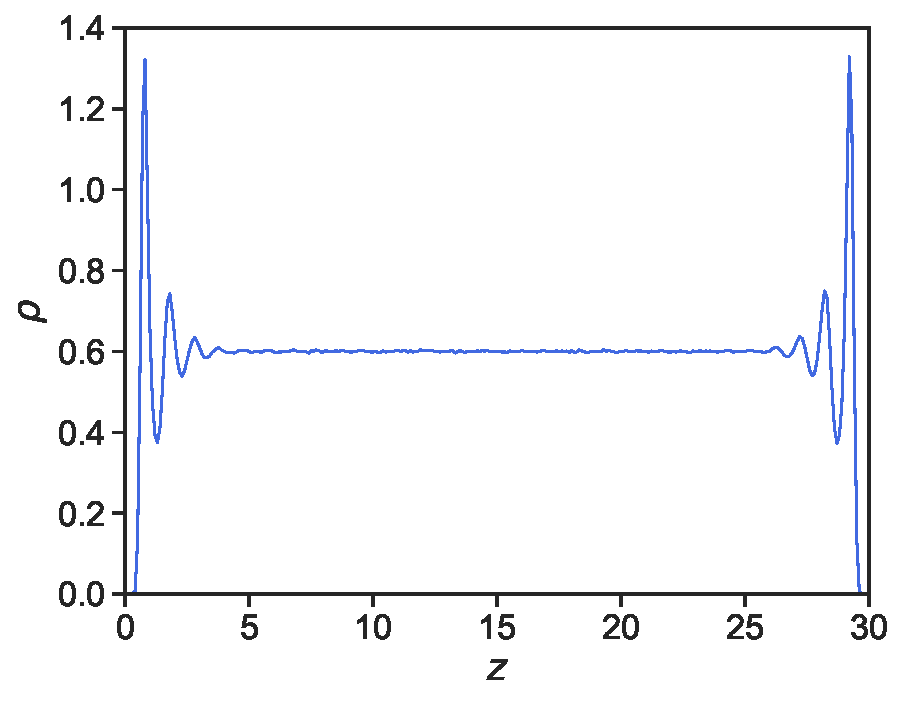
\includegraphics[width=0.48\linewidth]{Density-01sigma-2sigma-defensa}
\end{figure}
    \begin{itemize}
    \item DFT para situaciones de equilibrio.
    \item DDFT para partículas coloidales pero no para fluidos simples en contacto con sólidos. 
    \end{itemize}
\end{frame}

\begin{frame}{Velocidad de deslizamiento}
  La velocidad del fluido cerca de la pared es distinta de cero.
  \begin{itemize}
    \item<1-> Condición de contorno de \textit{slip}
          \begin{align}
            \delta\frac{\partial v}{\partial z}=v_{\rm des}, && \delta =\frac{\eta}{\gamma} \nonumber
          \end{align}
        %\item<4-> Bocquet y Barrat \cite{Bocquet1993}
        \item<2-> Bocquet y Barrat [Bocquet 1993]
\begin{align}
  \gamma=\frac{1}{Sk_BT}\int_0^{\tau} dt \llangle \hat{F}^x(t)\hat{F}^x\rrangle
\nonumber
\end{align}
      %\item<5-> Fricción entre dos paredes (Petravic y Harrowell \cite{Petravic2007}).
      \item<3-> Fricción entre dos paredes [Petravic 2007].
      \item<4-> La expresión para $\gamma$ sufre del \alert{problema del \textit{plateau}}. 
    \end{itemize}
\end{frame}

%\begin{frame}{Hoja de ruta}
%  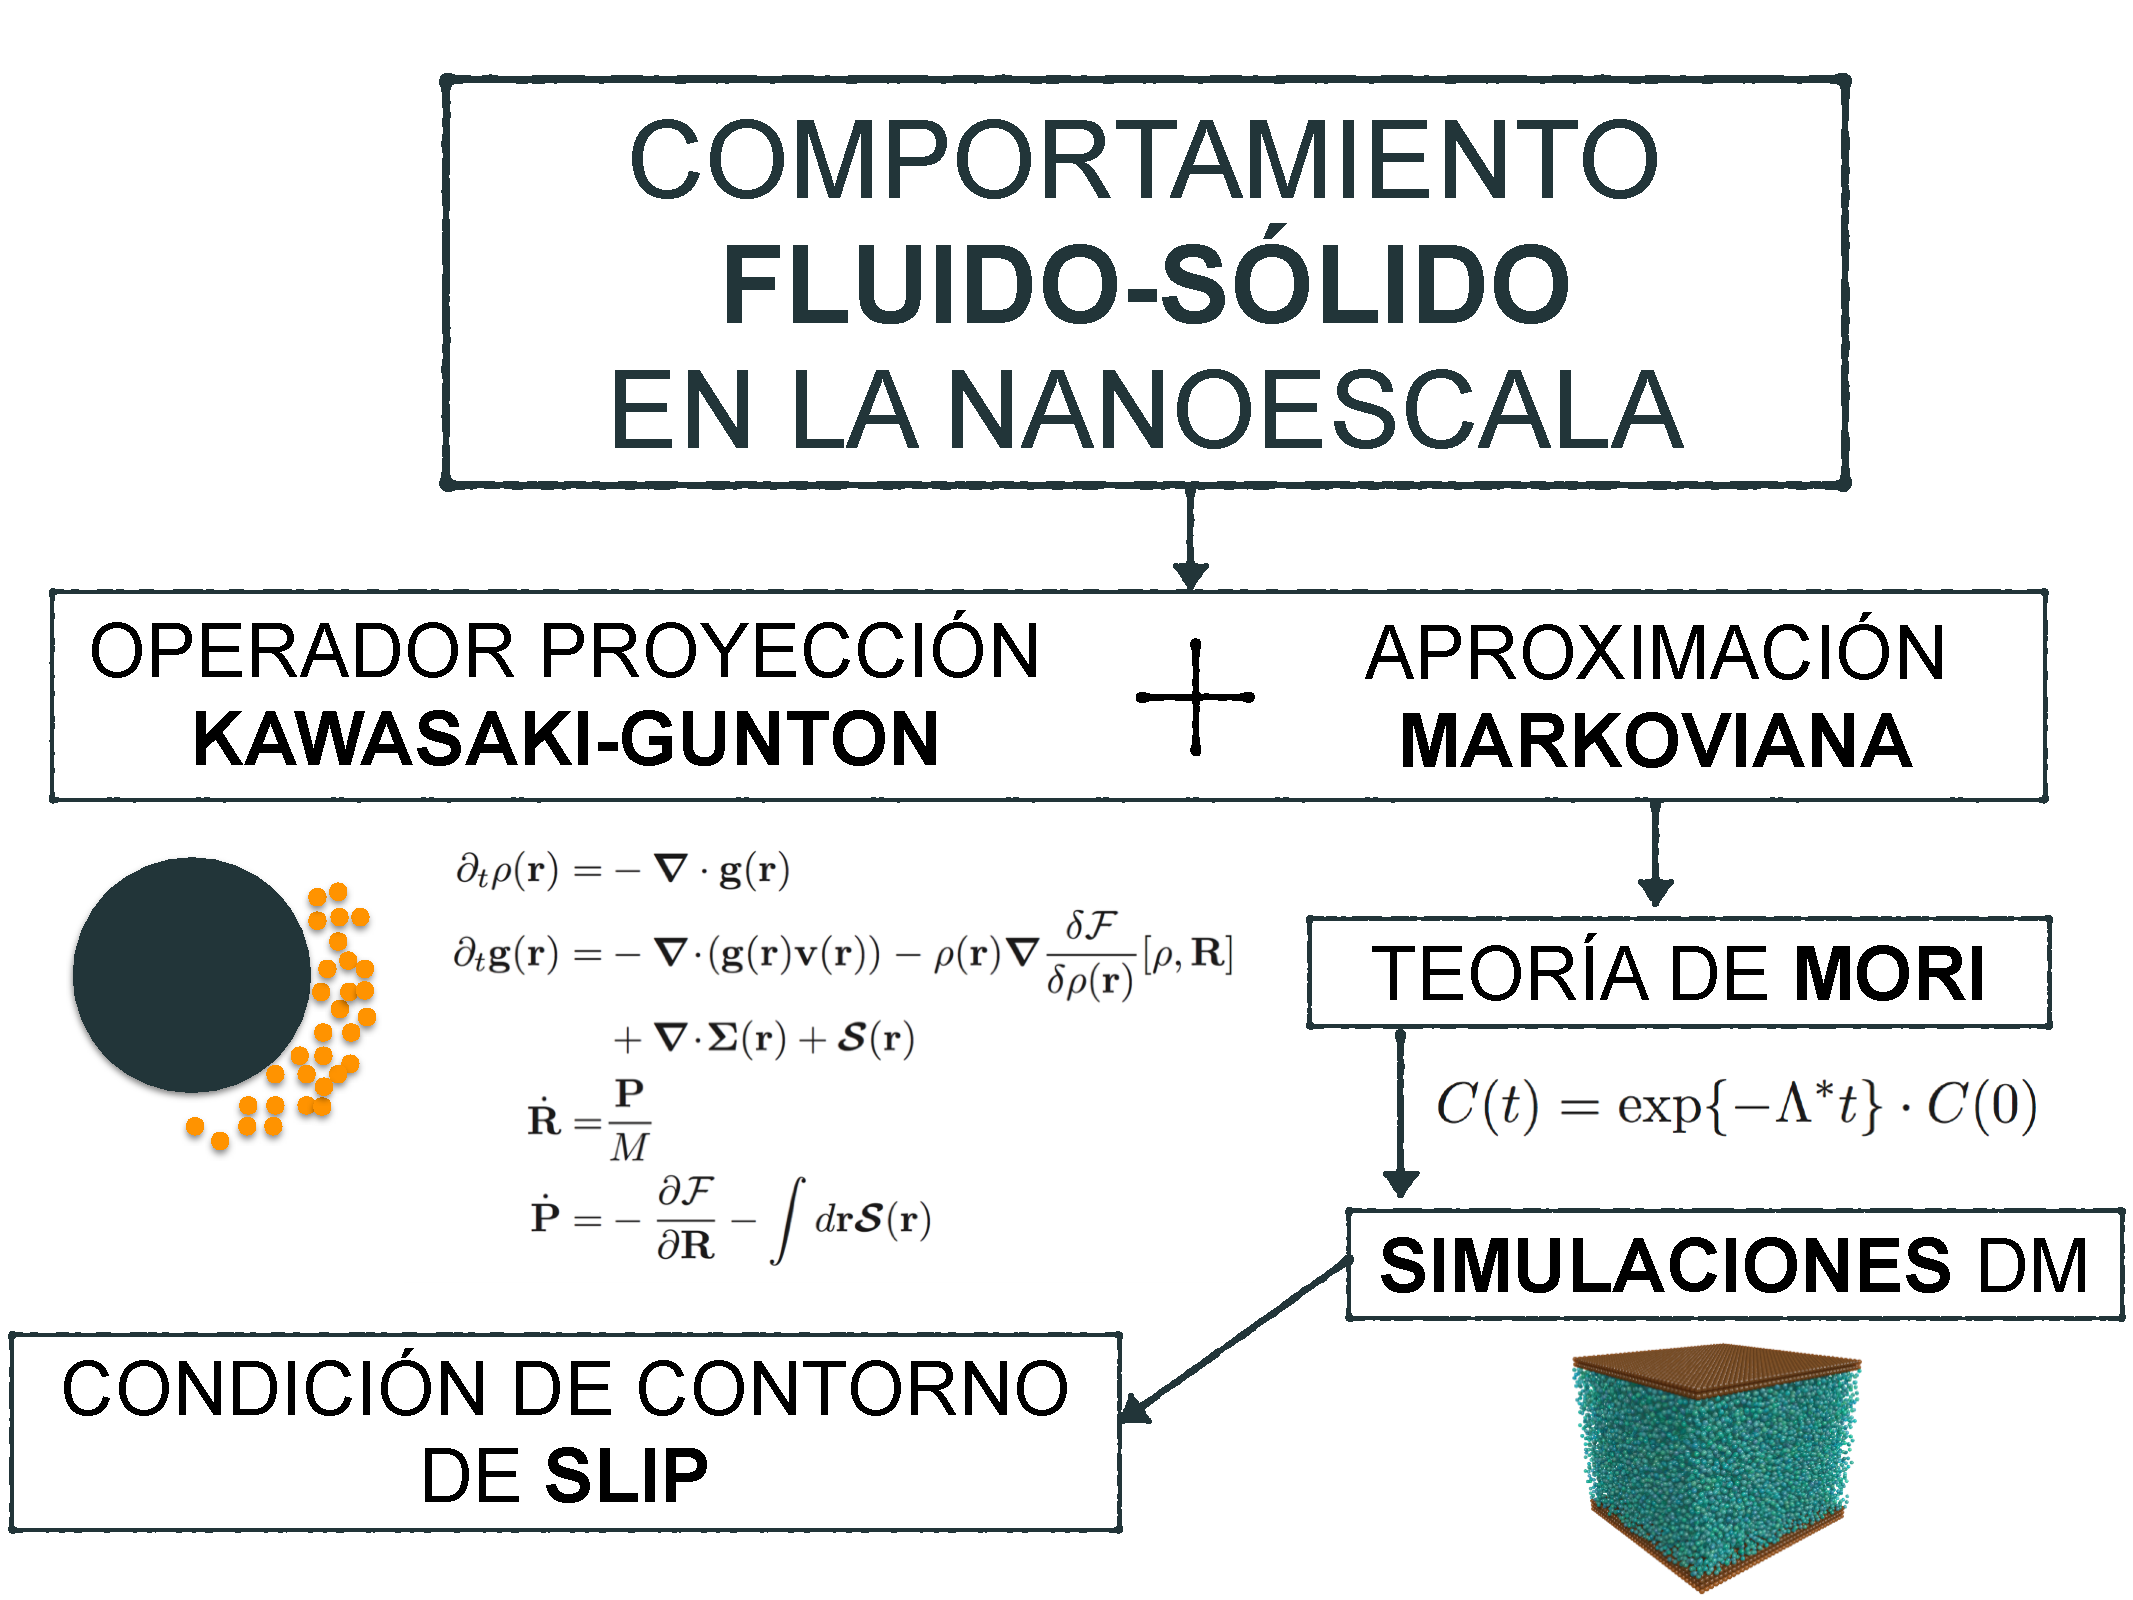
\includegraphics[width=\linewidth]{scheme-thesis-esp}
%\end{frame}
%
%\begin{frame}{Hoja de ruta}
%  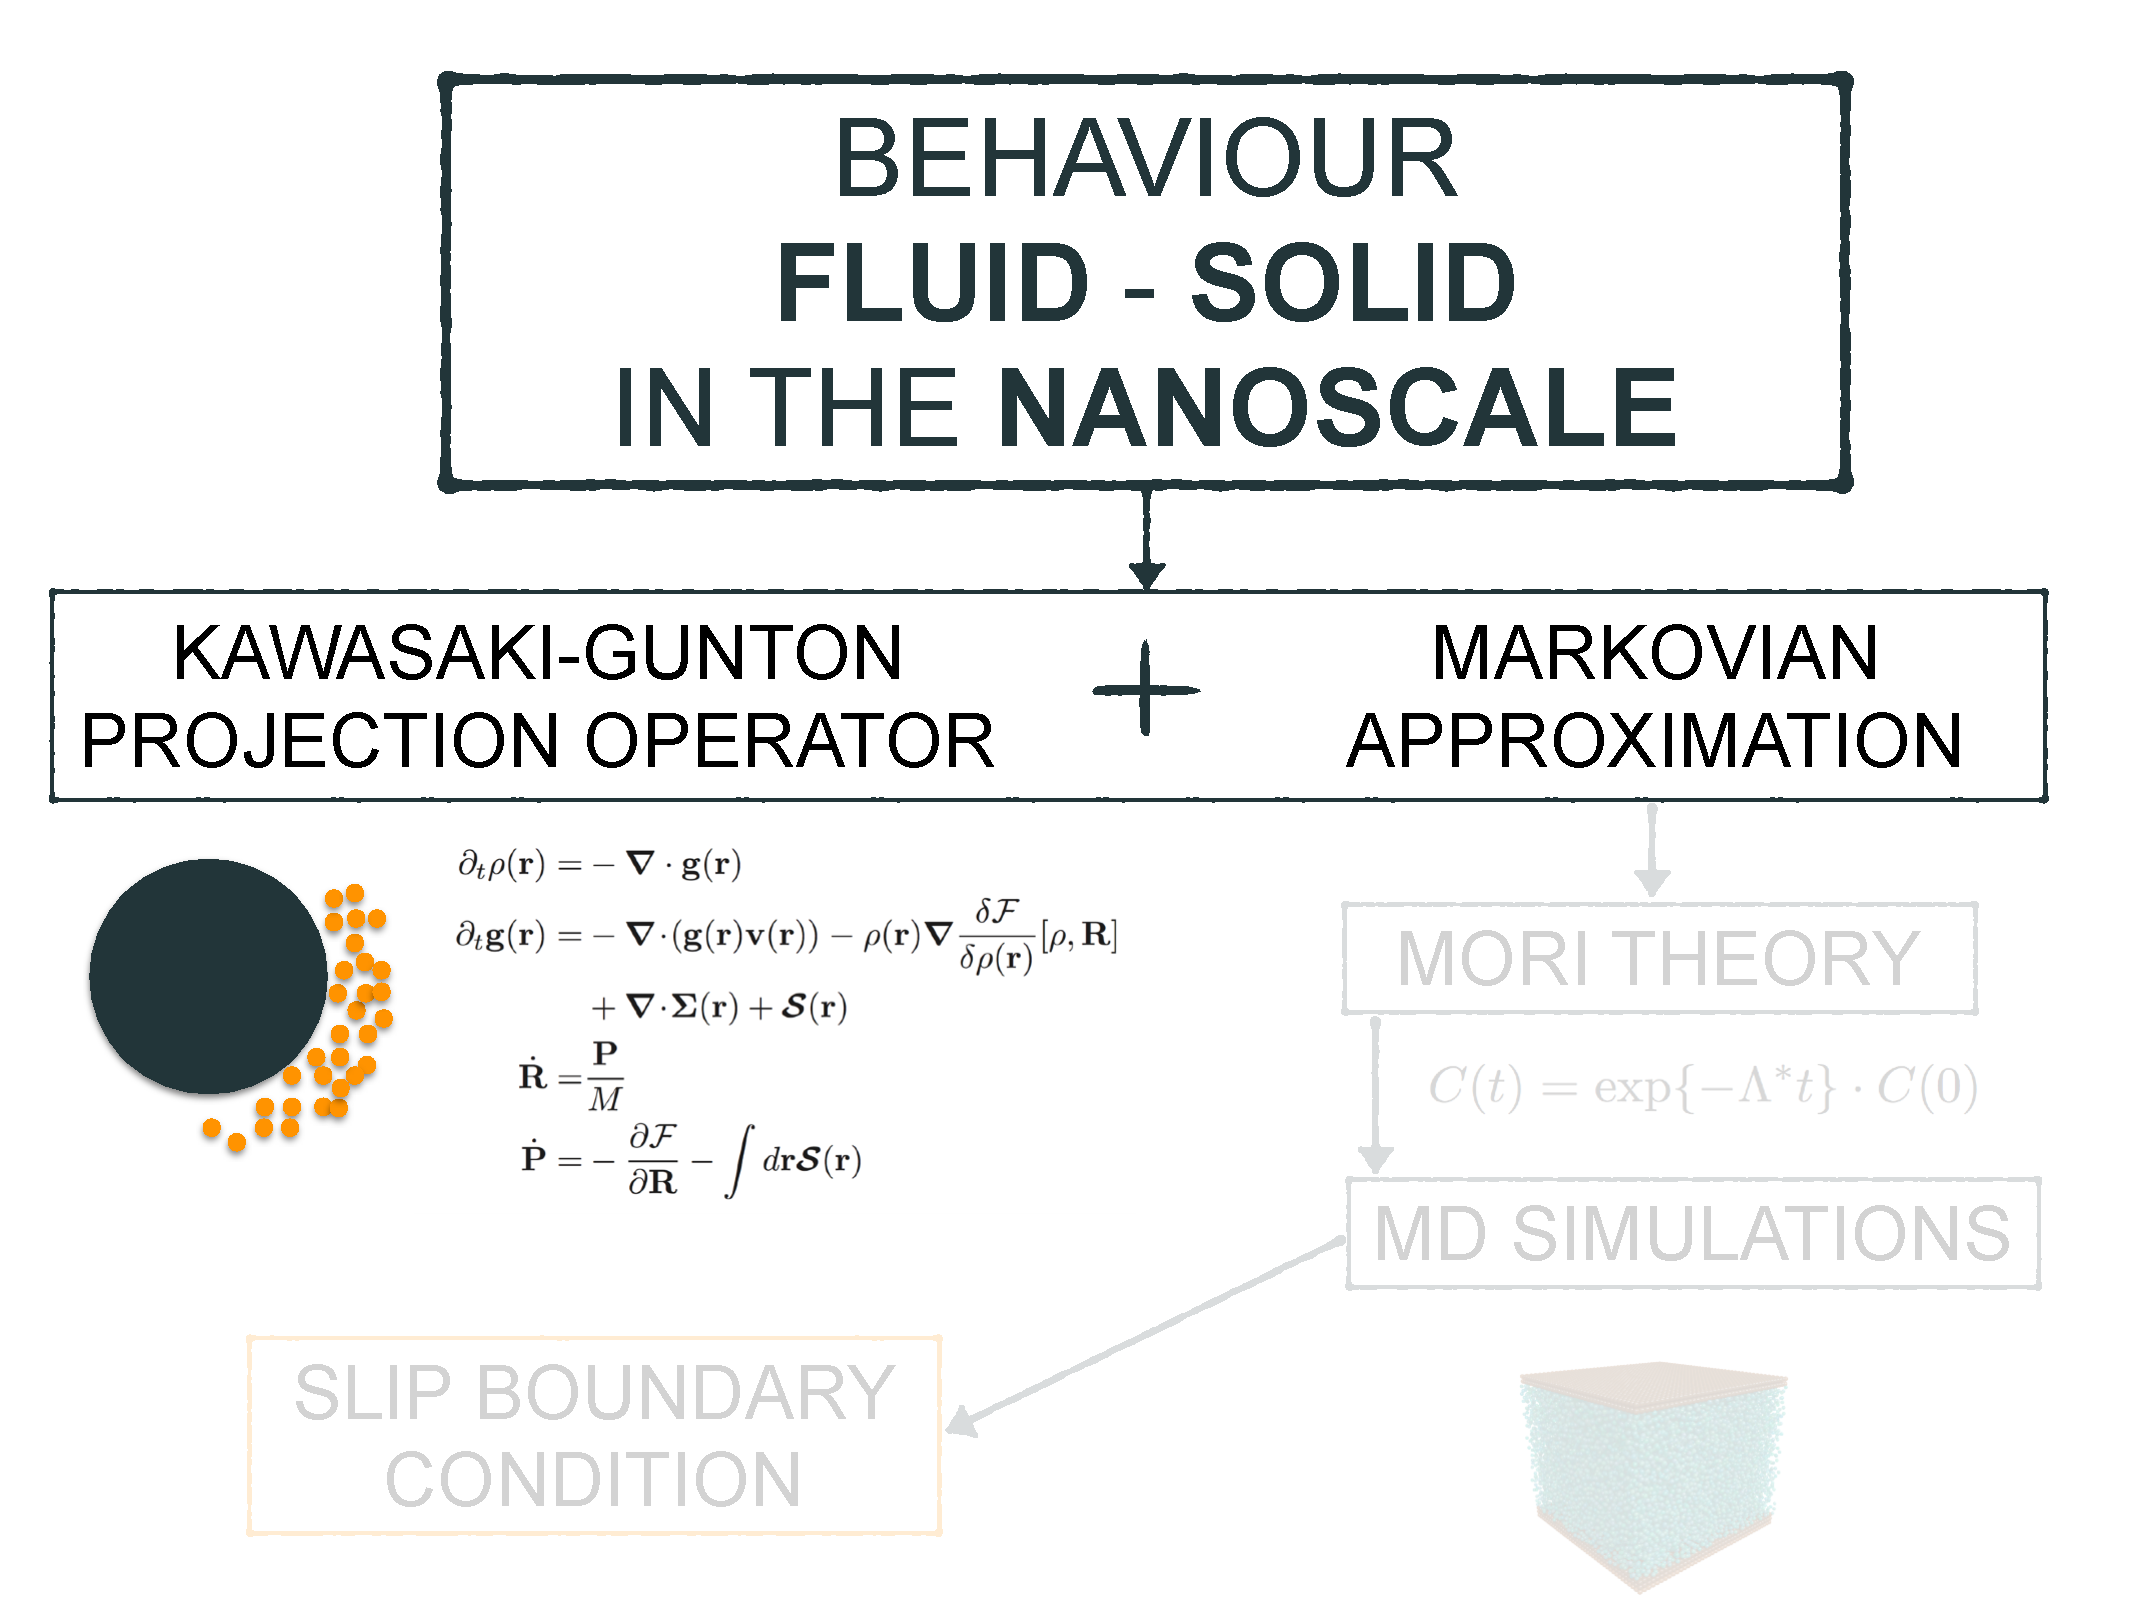
\includegraphics[width=\linewidth]{scheme-thesis-kawasaki}
%\end{frame}

\begin{frame}{Líneas de investigación}
  \textbf{Estudio del comportamiento de un fluido en contacto con un sólido en la nanoescala.}
  \begin{itemize}
    \item<1-> \alert{Kawasaki-Gunton} y aproximación Markoviana: Ecuaciones de la nanohidrodinámica que generalizan DFT para un fluido simple en movimiento en presencia de un sólido.
    \item<2-> Teoría discreta más simple: \alert{geometrías planas}.
    \item<3-> \alert{Teoría de Mori} con aproximación Markoviana. 
      \begin{align}
        C(t)=\exp\{\Lambda^*t\}\cdot C(0)
        \nonumber
      \end{align}
    \item<4-> \alert{Simulaciones}
      \begin{itemize}
        \item Fluido no confinado. 
        \item Fluido en contacto con paredes. 
      \end{itemize}
    \item<5-> \alert{Condición de contorno} de \textit{slip}. 
  \end{itemize}
\end{frame}

\section{Teoría hidrodinámica para fluidos cerca de sólidos}
\begin{frame}{El sistema}
  \begin{itemize}
    \item<1-> \alert{Objetivo}: Derivar ecuaciones de la hidrodinámica a partir de las ecuaciones de Hamilton. 
    \item<2-> Estudiamos un fluido de $N$ partículas en contacto con una esfera sólida compuesta por $N'$ partículas.
    %\item $z= ({\bf q}_i, {\bf p}_i)$ y $z'= ({\bf q}_{i'}, {\bf p}_{i'})$
  \begin{figure}
  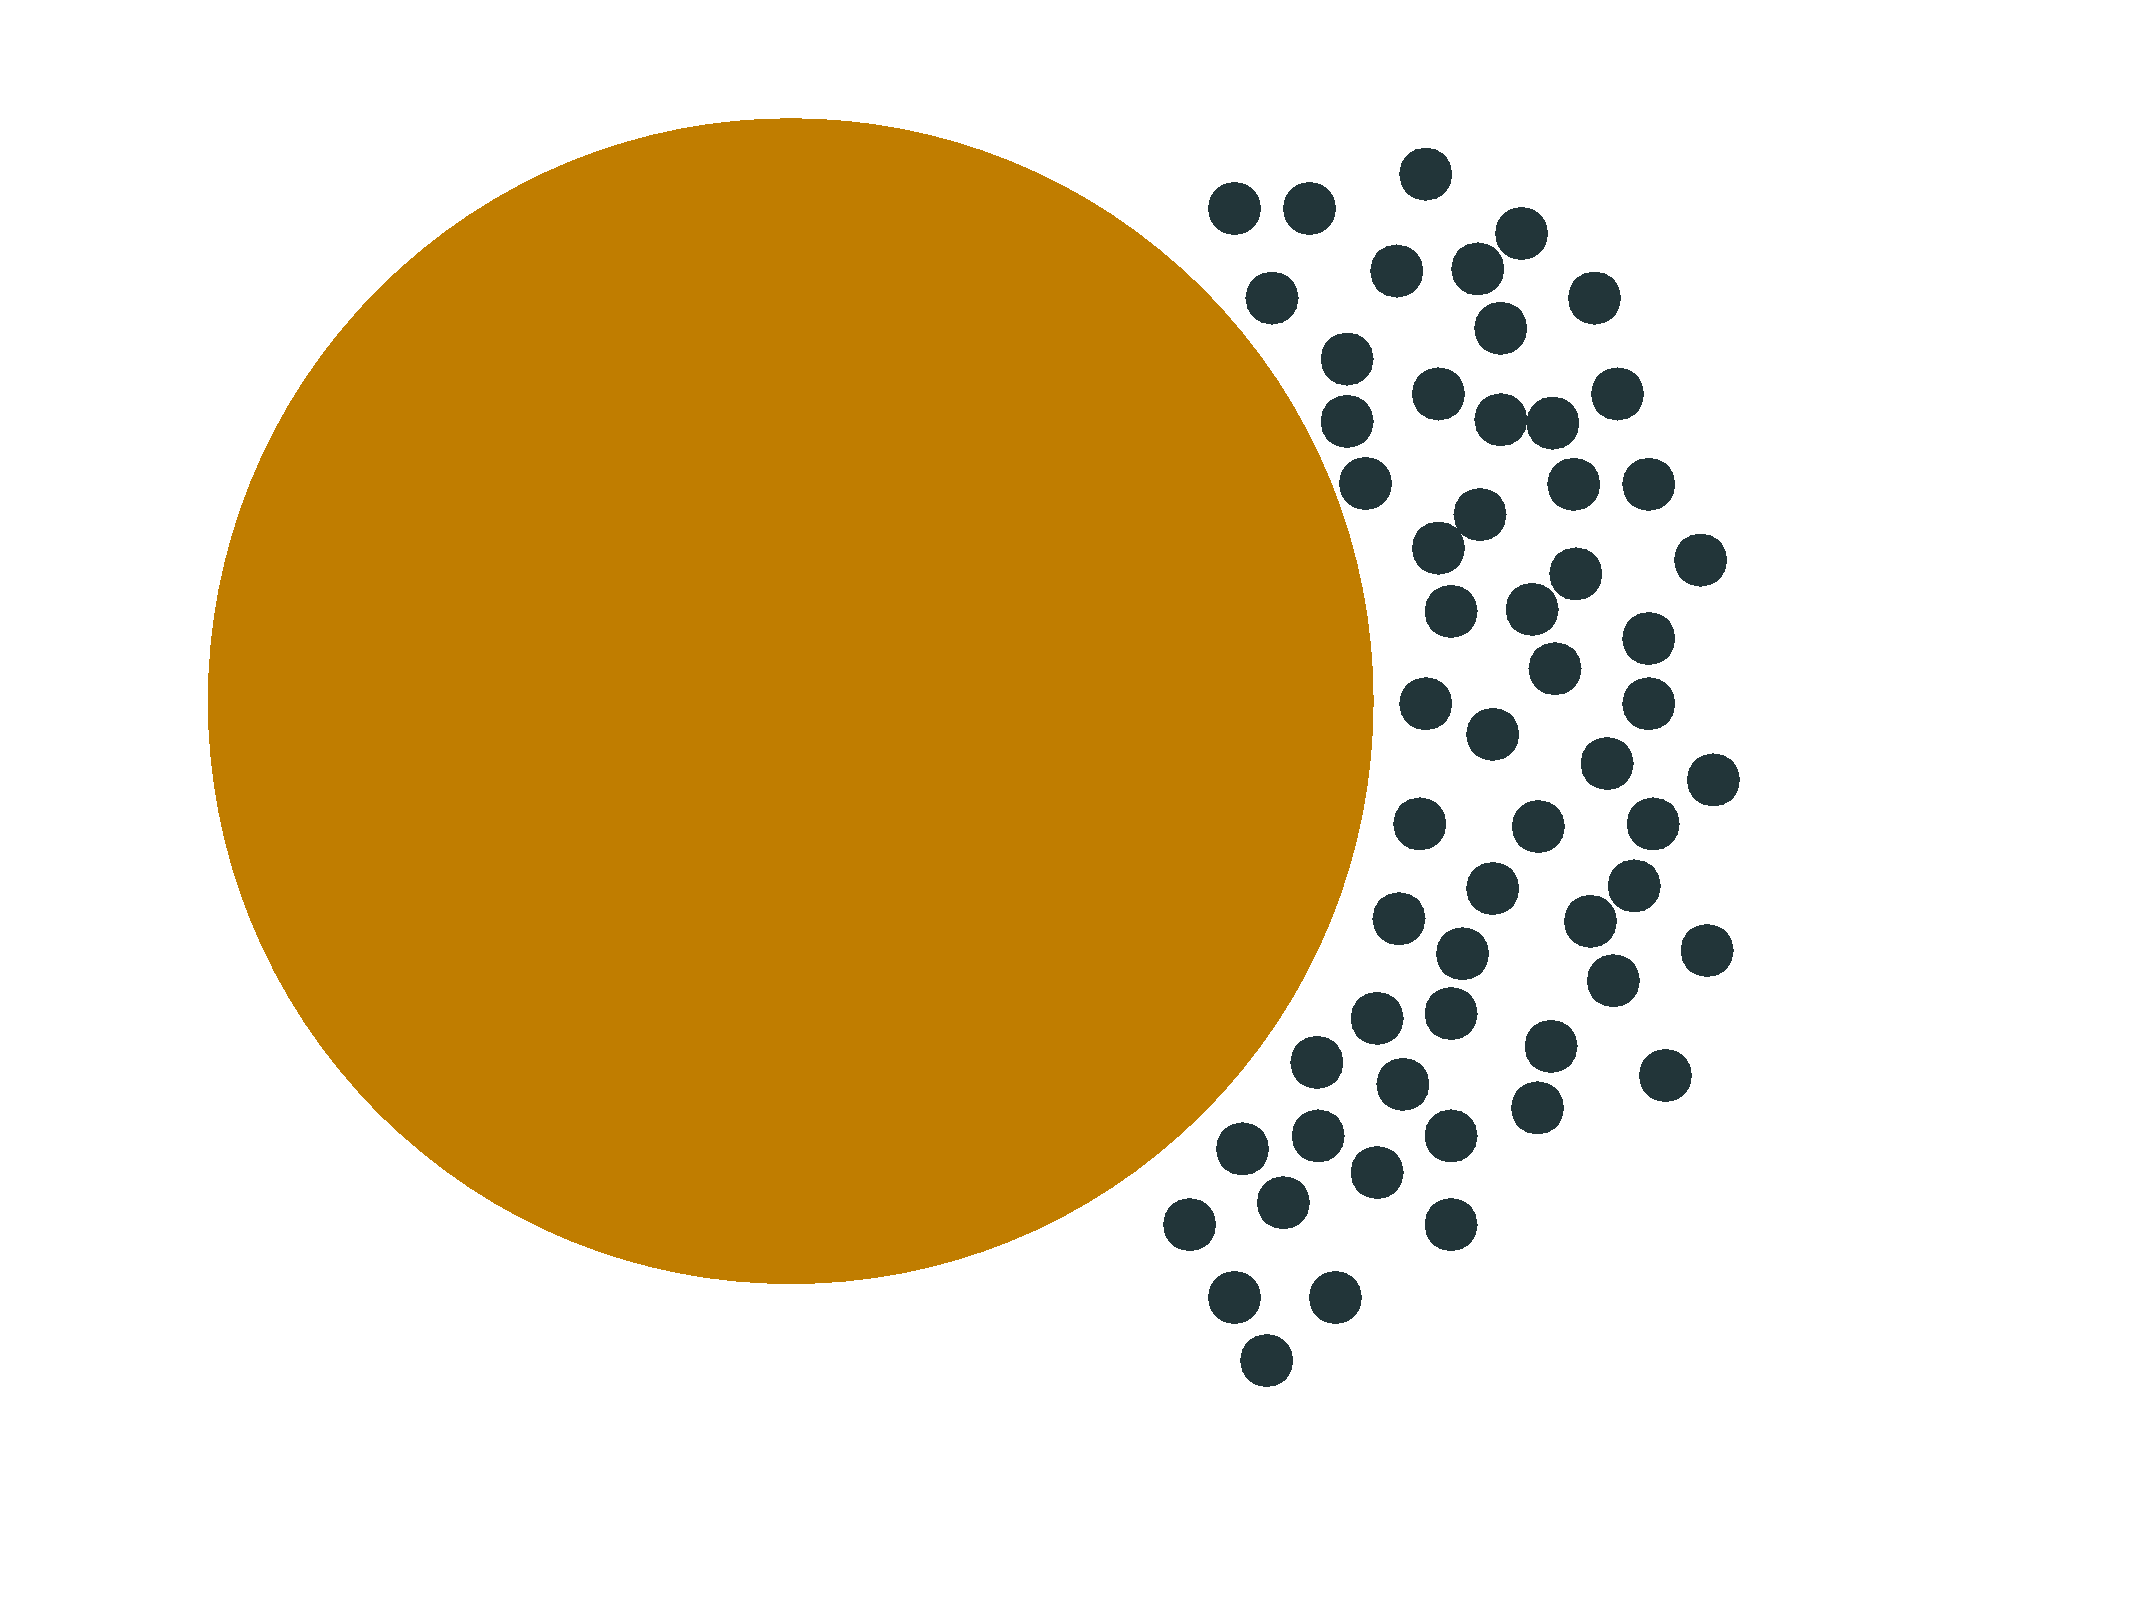
\includegraphics[width=.6\linewidth]{esfera}
  \end{figure}
  \end{itemize}
\end{frame}
   
   \begin{frame}{Las variables relevantes}
     \begin{itemize}
    \item<1-> Variables relevantes
      \begin{align}
        \hat{\rho}_{\bf r}(z) &=\sum^{N}_im\delta({\bf r}-{\bf q}_i)
      &&\hat{\bf R}(z)=\frac{1}{N'}\sum_{i'}^{N'}{\bf q}_{i'}
      \nonumber\\
        \hat{\bf g}_{\bf r}(z) &=\sum^{N}_i{\bf p}_i\delta({\bf r}-{\bf q}_i)
      &&\hat{\bf P}(z)=\sum_{i'}^{N'}{\bf p}_{i'}
      \nonumber
      \end{align}
    \item<2-> Derivadas temporales de las variables relevantes
      \begin{align}
        i{\cal L} \hat{\rho}_{\bf r}(z) &= -\boldsymbol{\nabla}\esc\hat{\bf g}_{\bf r}(z)
        && i{\cal L}\hat{\bf R}(z) =\frac{\hat{\bf P}(z)}{M}
      \nonumber\\
      i{\cal L}\hat{\bf g}_{\bf r}(z)
          &=-\boldsymbol{\nabla}\cdot \hat{\boldsymbol{\sigma}}_{\bf r}(z)+\hat{{\bf F}}^{\rm s\to l}_{\bf r}(z) 
        &&i{\cal L}\hat{\bf P}(z) =-\int  d{\bf r} \hat{\bf F}^{\rm s\to l}_{\bf r}(z)
         \nonumber
\end{align}
    \end{itemize}
\end{frame}

\begin{frame}{Operador de proyección de Kawasaki-Gunton}
  \begin{itemize}
    %\item<1-> Kawasaki-Gunton y aproximación Markoviana 
      %Si hay separación de escalas temporales entre la evolución de los promedios de las variables relevantes, $a_i$, y el decaimiento del kernel de memoria 
    \item<1-> Ecuaciones de evolución para los promedios de las variables relevantes, $a_i(t)$
\begin{equation}
  \frac{\partial}{\partial t}a_i(t) = {\color{blue} v_i(t)}+ {\color{red} \sum_j D_{ij}(t) \lambda_j(t)}
\nonumber
\end{equation}
\item<2-> {\color{blue} Término reversible}: 
  %\begin{align}
  $v_i={\rm Tr}[\overline{\rho}_t i{\cal L}\hat{A}_i]$
   % \nonumber
  %\end{align}
  \\En donde 
  ${\rm Tr}\left[\cdots\right]=\sum_{N=0}^\infty \frac{1}{N!h^{3N}}
\int dz\cdots$
\item<3-> Colectividad relevante 
  \begin{equation}
  \overline{\rho}(z) = \frac{1}{Z[\lambda]} \rho_0\exp\{-\lambda\!\cdot\!\hat{A}(z)\}
  \nonumber
  \end{equation}
\item<4-> Promedios variables relevantes: $a_i={\rm Tr}[\bar{\rho}\hat{A}_i]={\rm Tr}[\rho\hat{A}_i]$
\item<5-> {\color{red} La matriz disipativa} viene dada por la fórmula de  Green-Kubo
\begin{equation}
D_{ij}(t)=\int_0^{\Delta t} dt'\left\langle 
{\cal Q}_t i{\cal L}\hat{A}_j\exp\{i{\cal L}t'\}{\cal Q}_t i{\cal L}\hat{A}_i
\right\rangle^{\lambda(t)}
\label{dij}
\nonumber
\end{equation}
%\item<5-> El operador de proyección de Kawasaki-Gunton  
%  \begin{align}
%    {\cal Q}_{t'}\hat{F}(z) &= \hat{F}(z)- {\rm Tr}[\overline{\rho}_{t'} \hat{F}]
%  -\sum_i(\hat{A}_i(z)-a_i(t'))\frac{\partial }{\partial a_i(t')}
%  {\rm Tr}[\overline{\rho}_{t'} \hat{F}]
%  \label{Q}
%  \nonumber
%  \end{align}
\end{itemize}
\end{frame}

\begin{frame}{Ecuaciones de la nanohidrodinámica}
\begin{align}
  \partial_t\rho({\bf r})=&{\color{blue} -\boldsymbol{\nabla}\cdot{\bf g}({\bf r})}
\nonumber\\
\partial_t{\bf g}({\bf r})=&{\color{blue} -\boldsymbol{\nabla}\esc{\left({\bf g}({\bf r}){\bf v}({\bf r})\right)}
-\rho({\bf r})\boldsymbol{\nabla}\frac{\delta {\cal F}}{\delta\rho({\bf r})}[\rho,{\bf R}]}
{\color{red} +\boldsymbol{\nabla}\esc\boldsymbol{\Sigma}({\bf r})+\boldsymbol{{\cal S}}({\bf r})}
\nonumber\\
\dot{\bf R}=&{\color{blue} \frac{\bf P}{M}}
\nonumber\\
\dot{\bf P}=&{\color{blue} -\frac{\partial {\cal F}}{\partial {\bf R}}}
{\color{red} -\int d {{\bf r}}\boldsymbol{{\cal S}}({\bf r})}
\nonumber
\end{align}

\begin{itemize}
  \item ${\cal F}[\rho, {\bf R}]$: funcional de energía libre de un fluido en presencia de una esfera sólida (DFT).
  \item $\boldsymbol{\Sigma}({\bf r})$: tensor de tensiones del fluido. 
  \item $\boldsymbol{{\cal S}}({\bf r})$: fuerza irreversible sobre el fluido. 
\end{itemize}
\end{frame}

\begin{frame}{El tensor de tensiones del fluido y la fuerza irreversible}
  \begin{itemize}
    \item<1-> El tensor de tensiones del fluido ${\color{red} \boldsymbol{\Sigma}({\bf r})}$ 
  \begin{align}
  \boldsymbol{\Sigma}^{\alpha\beta}({\bf r})&=
\int d{\bf r}'
\boldsymbol{\eta}^{\alpha\beta\alpha'\beta'}_{{\bf r}{\bf r}'}
\boldsymbol{\nabla}_{{\bf r}'}^{\beta'}{\bf v}^{\alpha'}({\bf r}')
\nonumber
\end{align}
\item<2-> Fuerza irreversible sobre el fluido ${\color{red} {\cal S}({\bf r})}$
\begin{align}
  \boldsymbol{{\cal S}}^\alpha({\bf r})=&
-\int d{\bf r}'{\bf G}^{\alpha\alpha'\beta'}_{{\bf r}{\bf r}'}
\boldsymbol{\nabla}_{{\bf r}'}^{\beta'} {\bf v}^{\alpha'}({\bf r}')
+\boldsymbol{\nabla}_{{\bf r}}^{\beta}\int d{\bf r}'{\bf H}^{\alpha\beta\alpha'}_{{\bf r}{\bf r}'}
( {\bf v}^{\alpha'}({\bf r}')-{\bf V}^{\alpha'})
\nonumber\\
&-\int d{\bf r}'
\boldsymbol{\gamma}^{\alpha\alpha'}_{{\bf r}{\bf r}'}( {\bf v}^{\alpha'}({\bf r}')
-{\bf V}^{\alpha'})
\nonumber
\end{align}
\end{itemize}
\end{frame}

\begin{frame}{Los kernels de transporte}
%Comentar que los kernels H,G y gamma estarían muy localizados cerca de las paredes porque está involucrada la fuerza. 
\begin{align}
  \boldsymbol{\eta}_{{\bf  r}{\bf r}'} &\equiv
\frac{1}{k_BT}\int_0^{\Delta t} dt'\langle 
{\cal Q}_t\hat{\boldsymbol{\sigma}}_{{\bf r}}(t')
{\cal Q}_t\hat{\boldsymbol{\sigma}}_{{\bf r}'}\rangle^{\lambda(t)}
\nonumber \\
{\bf H}_{{\bf r}{\bf r}'}&\equiv\frac{1}{k_BT}\int_0^{\Delta t} dt'
\langle {\cal Q}_t\hat{\boldsymbol{\sigma}}_{{\bf r}}(t')
{\cal Q}_t\hat{\bf F}^{\rm s\to l}_{{\bf r}'}\rangle^{\lambda(t)}
\nonumber\\
{\bf G}_{{\bf r}{\bf r}'}&\equiv\frac{1}{k_BT}\int_0^{\Delta t} dt'
\langle {\cal Q}_t\hat{\bf F}^{\rm s\to l}_{{\bf r}}(t')
{\cal Q}_t\hat{\boldsymbol{\sigma}}_{{\bf r}'}\rangle^{\lambda(t)}
\nonumber\\
\boldsymbol{\gamma}_{{\bf  r}{\bf r}'}&\equiv\frac{1}{k_BT}\int_0^{\Delta t} dt'
\langle 
{\cal Q}_t\hat{\bf F}^{\rm s\to l}_{{\bf r}}(t')
{\cal Q}_t\hat{\bf F}^{\rm s\to l}_{{\bf r}'}\rangle^{\lambda(t)}
\nonumber
\end{align}
\end{frame}

\metroset{background=dark}
\begin{frame}
  \begin{itemize}
    \item<1-> \alert{Generalización de la DFT} para un fluido simple en movimiento en presencia de una esfera sólida. 
    \item<2-> No hay condiciones de contorno. La interacción con el sólido es tenida en cuenta a través de \alert{fuerzas irreversibles} $\cal{S}({\bf r}).$ 
    \item<3-> D.Camargo, J.A. de la Torre,  D.Duque-Zumajo, P.Espa\~nol, R.Delgado-Buscalioni, and F. Chejne. Nanoscale hydrodynamics near solids. \textit{Journal of Chemical Physics}, 148(6), 2018.
  \end{itemize}

\end{frame}
\metroset{background=white}


%\begin{frame}{Algo}
%  \begin{itemize}
%    \item Generalización de DFT para fluidos simples en presencia de una esfera sólida de grandes dimensiones. 
%    \item Teoría continua para la evolución de las variables relevantes.
%    \item La única aproximación realizada es la Markoviana. 
%    \item Impracticable el cálculo de los kernels de transporte: no locales y de caracter tensorial. 
%    \item Teoría continua $\rightarrow$ No podemos calcular nada.
%    \item Si pudiéramos calcular algo sería muy costoso a nivel computacional. 
%  \end{itemize}
%\end{frame}

\begin{frame}{Necesidad de una teoría sencilla}
  %\begin{itemize}
    %\item[] La teoría presentada no puede ser validada a través de simulaciones:
    La teoría presentada no puede ser validada a través de simulaciones:
      \begin{enumerate}
        \item Teoría continua.
        \item Demasiada información en las ecs. hidrodinámicas: kernels de transporte no locales y de carácter tensorial. 
      \end{enumerate}
    %\item[] $\rightarrow$ Necesitamos una \alert{teoría más simple} (menos información que calcular) y \alert{discreta}. 
    $\rightarrow$ Necesitamos una \alert{teoría más simple} (menos información que calcular) y \alert{discreta}. 
  %\end{itemize}
\end{frame}

\section{Hidrodinámica discreta para flujos planos cerca de sólidos}

\begin{frame}{Teoría discreta de un caso sencillo}
  \begin{itemize}
    \item<1-> Paredes planas e isotrópicas. 
      \begin{figure}
        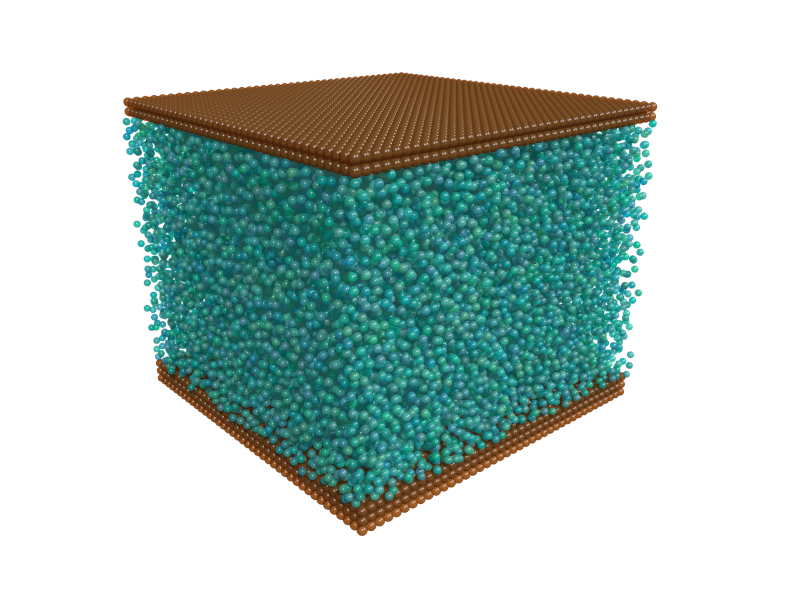
\includegraphics[width=.6\linewidth]{PRL3_gold2_wo_layers_wo_diffuse}
      \end{figure}
    \item<2-> Flujos planos $\rightarrow$ Invariancia traslacional en la dirección paralela a las paredes.
    %\item<3-> Teoría discreta para poder validarla a través de simulaciones de dinámica molecular.  
  \end{itemize}
\end{frame}

\begin{frame}{Discretización}
  %\begin{itemize}
    %\item 
  $N_{\rm bin}$ bines de dimensiones $L_x$, $L_y$, $\Delta z$, siendo $\Delta z = \frac{L_z}{N_{\rm bin}}$.
      \begin{center}
      %  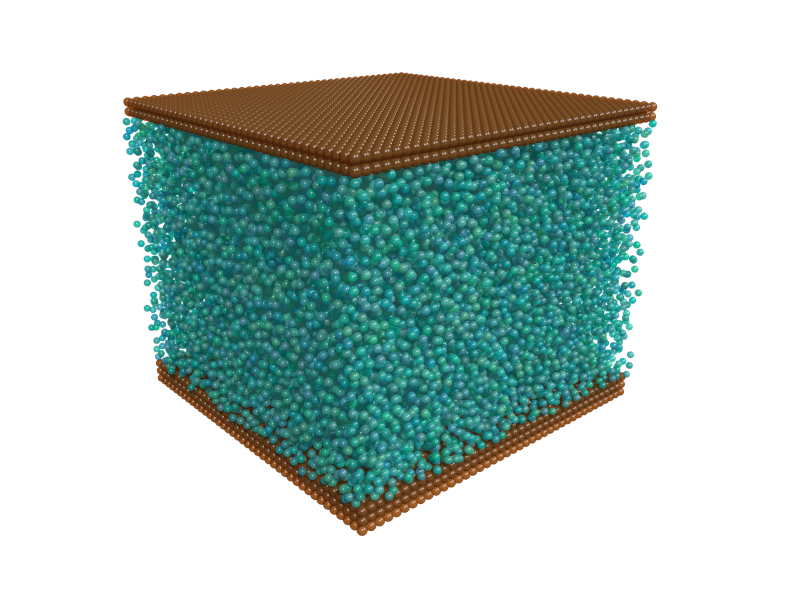
\includegraphics[width=.5\linewidth]{PRL3_gold2_wo_layers_wo_diffuse}
        %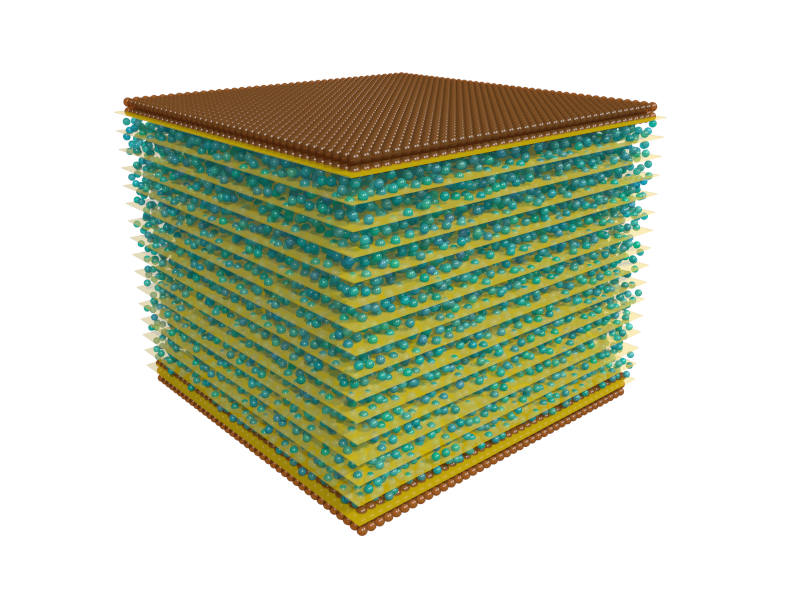
\includegraphics[width=.5\linewidth]{PRL3_gold2_wo_diffuse}
       % 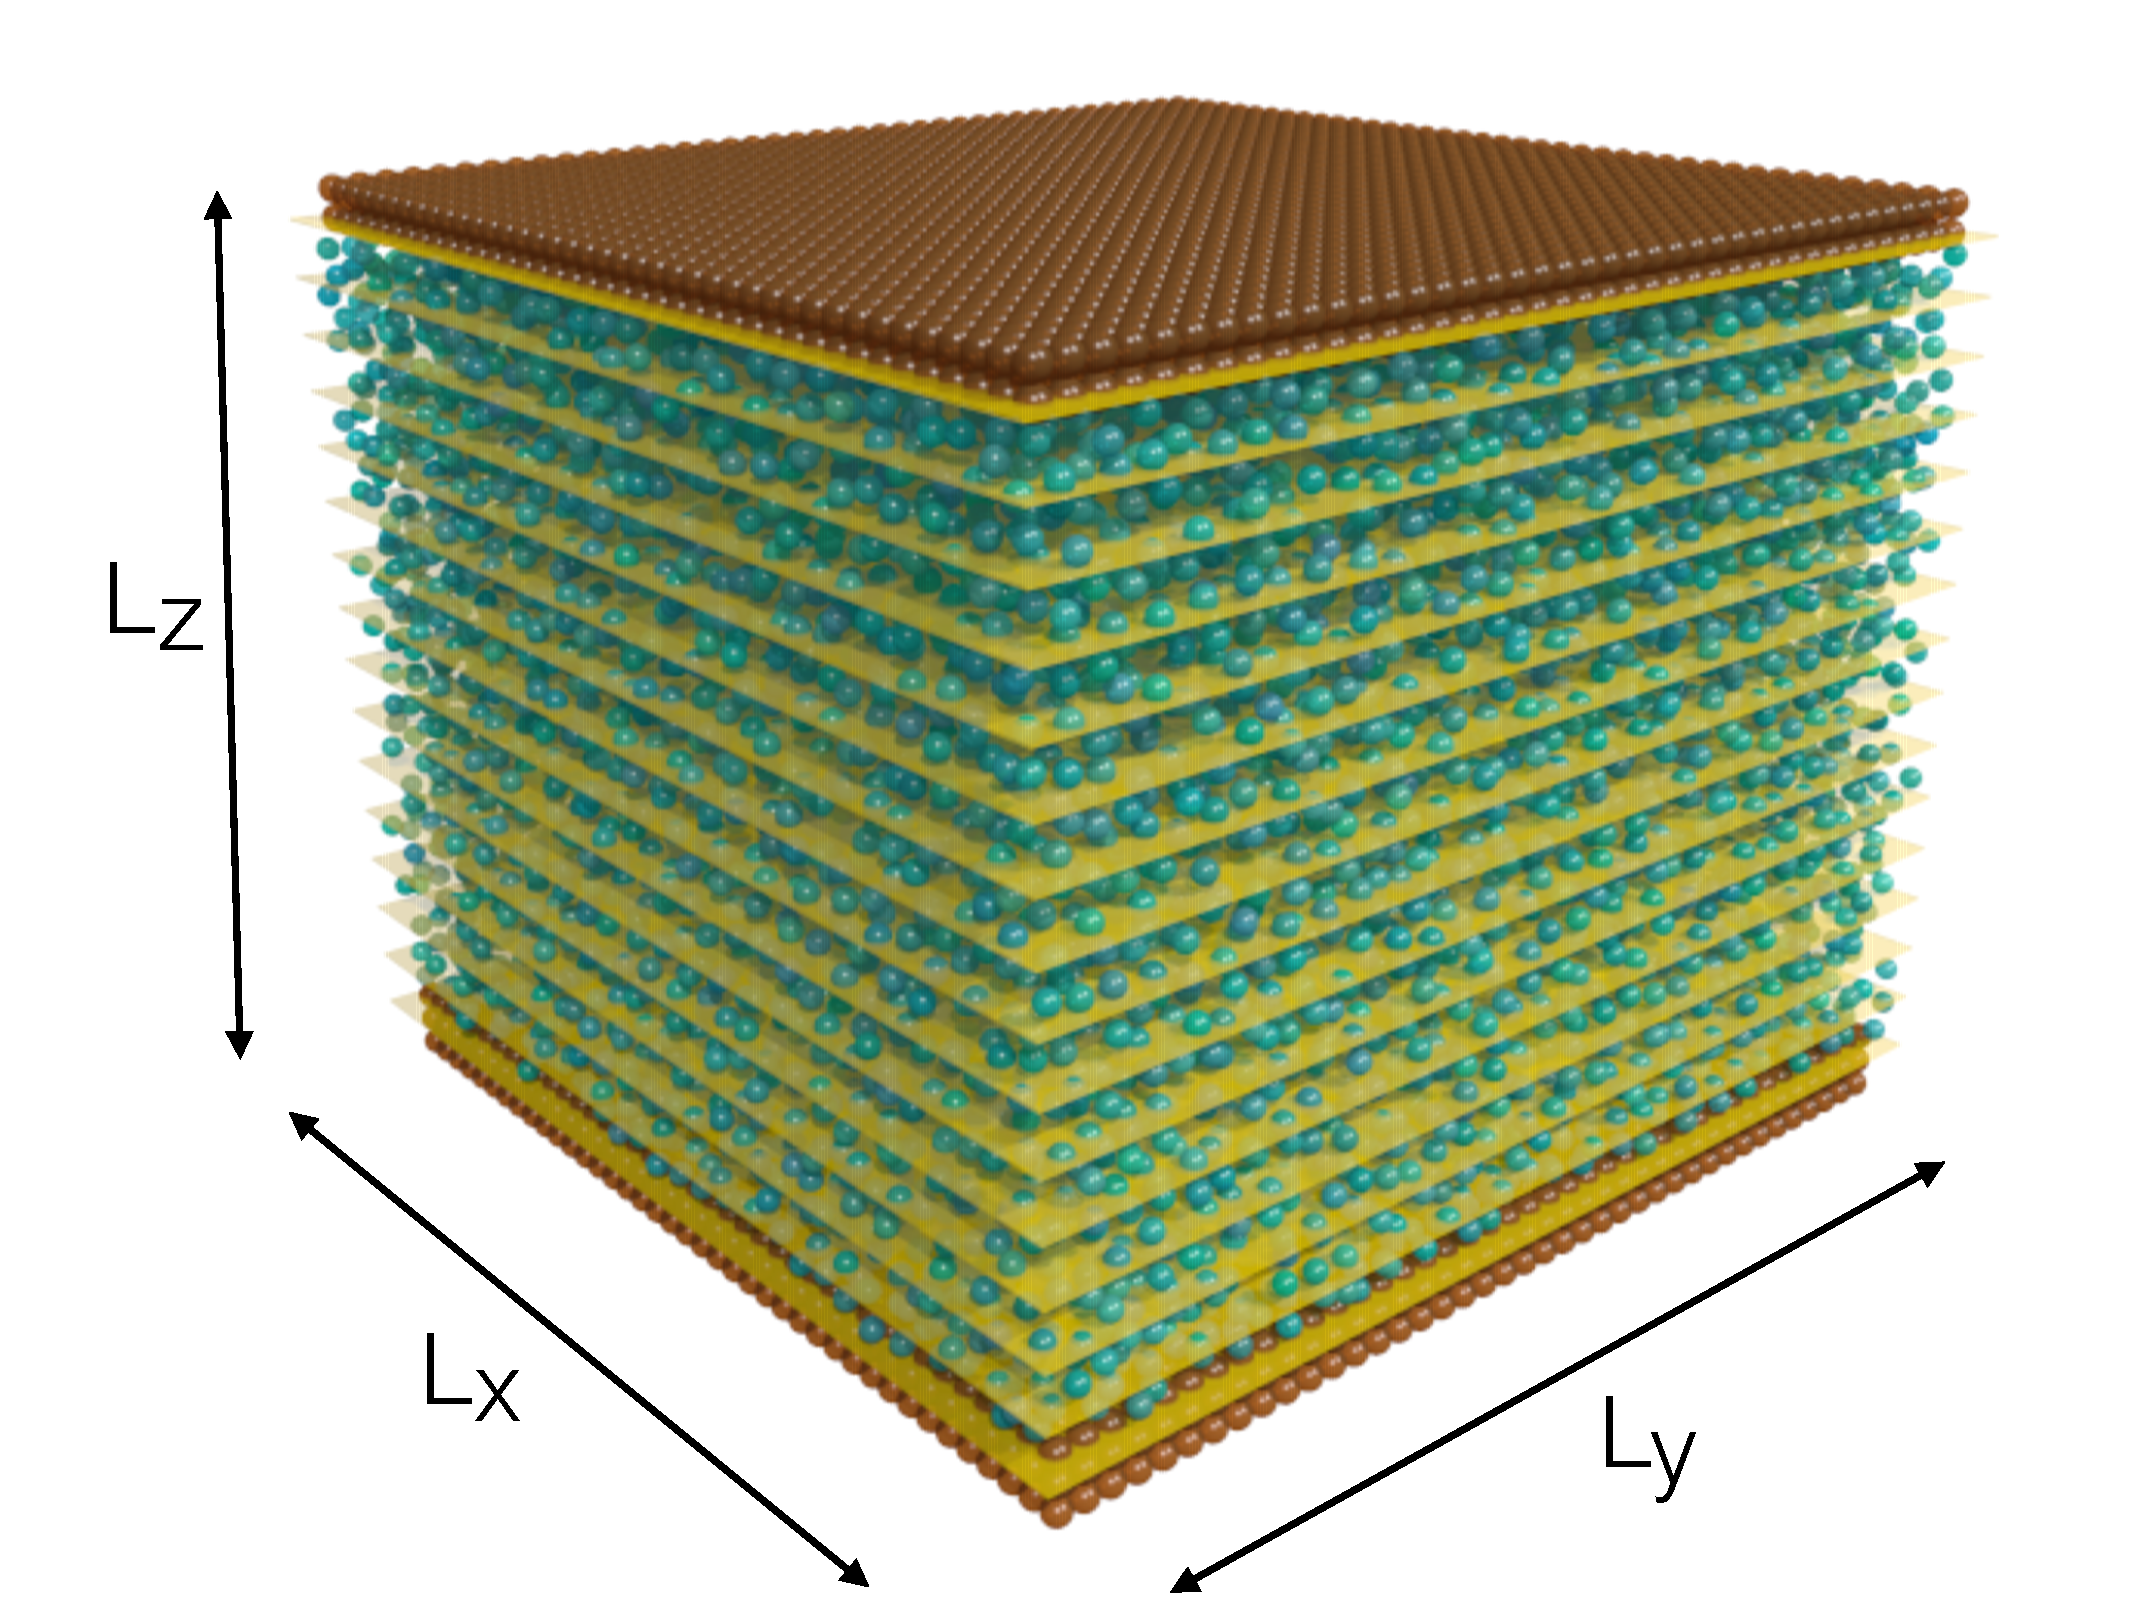
\includegraphics[width=.45\linewidth]{scheme-bines}
        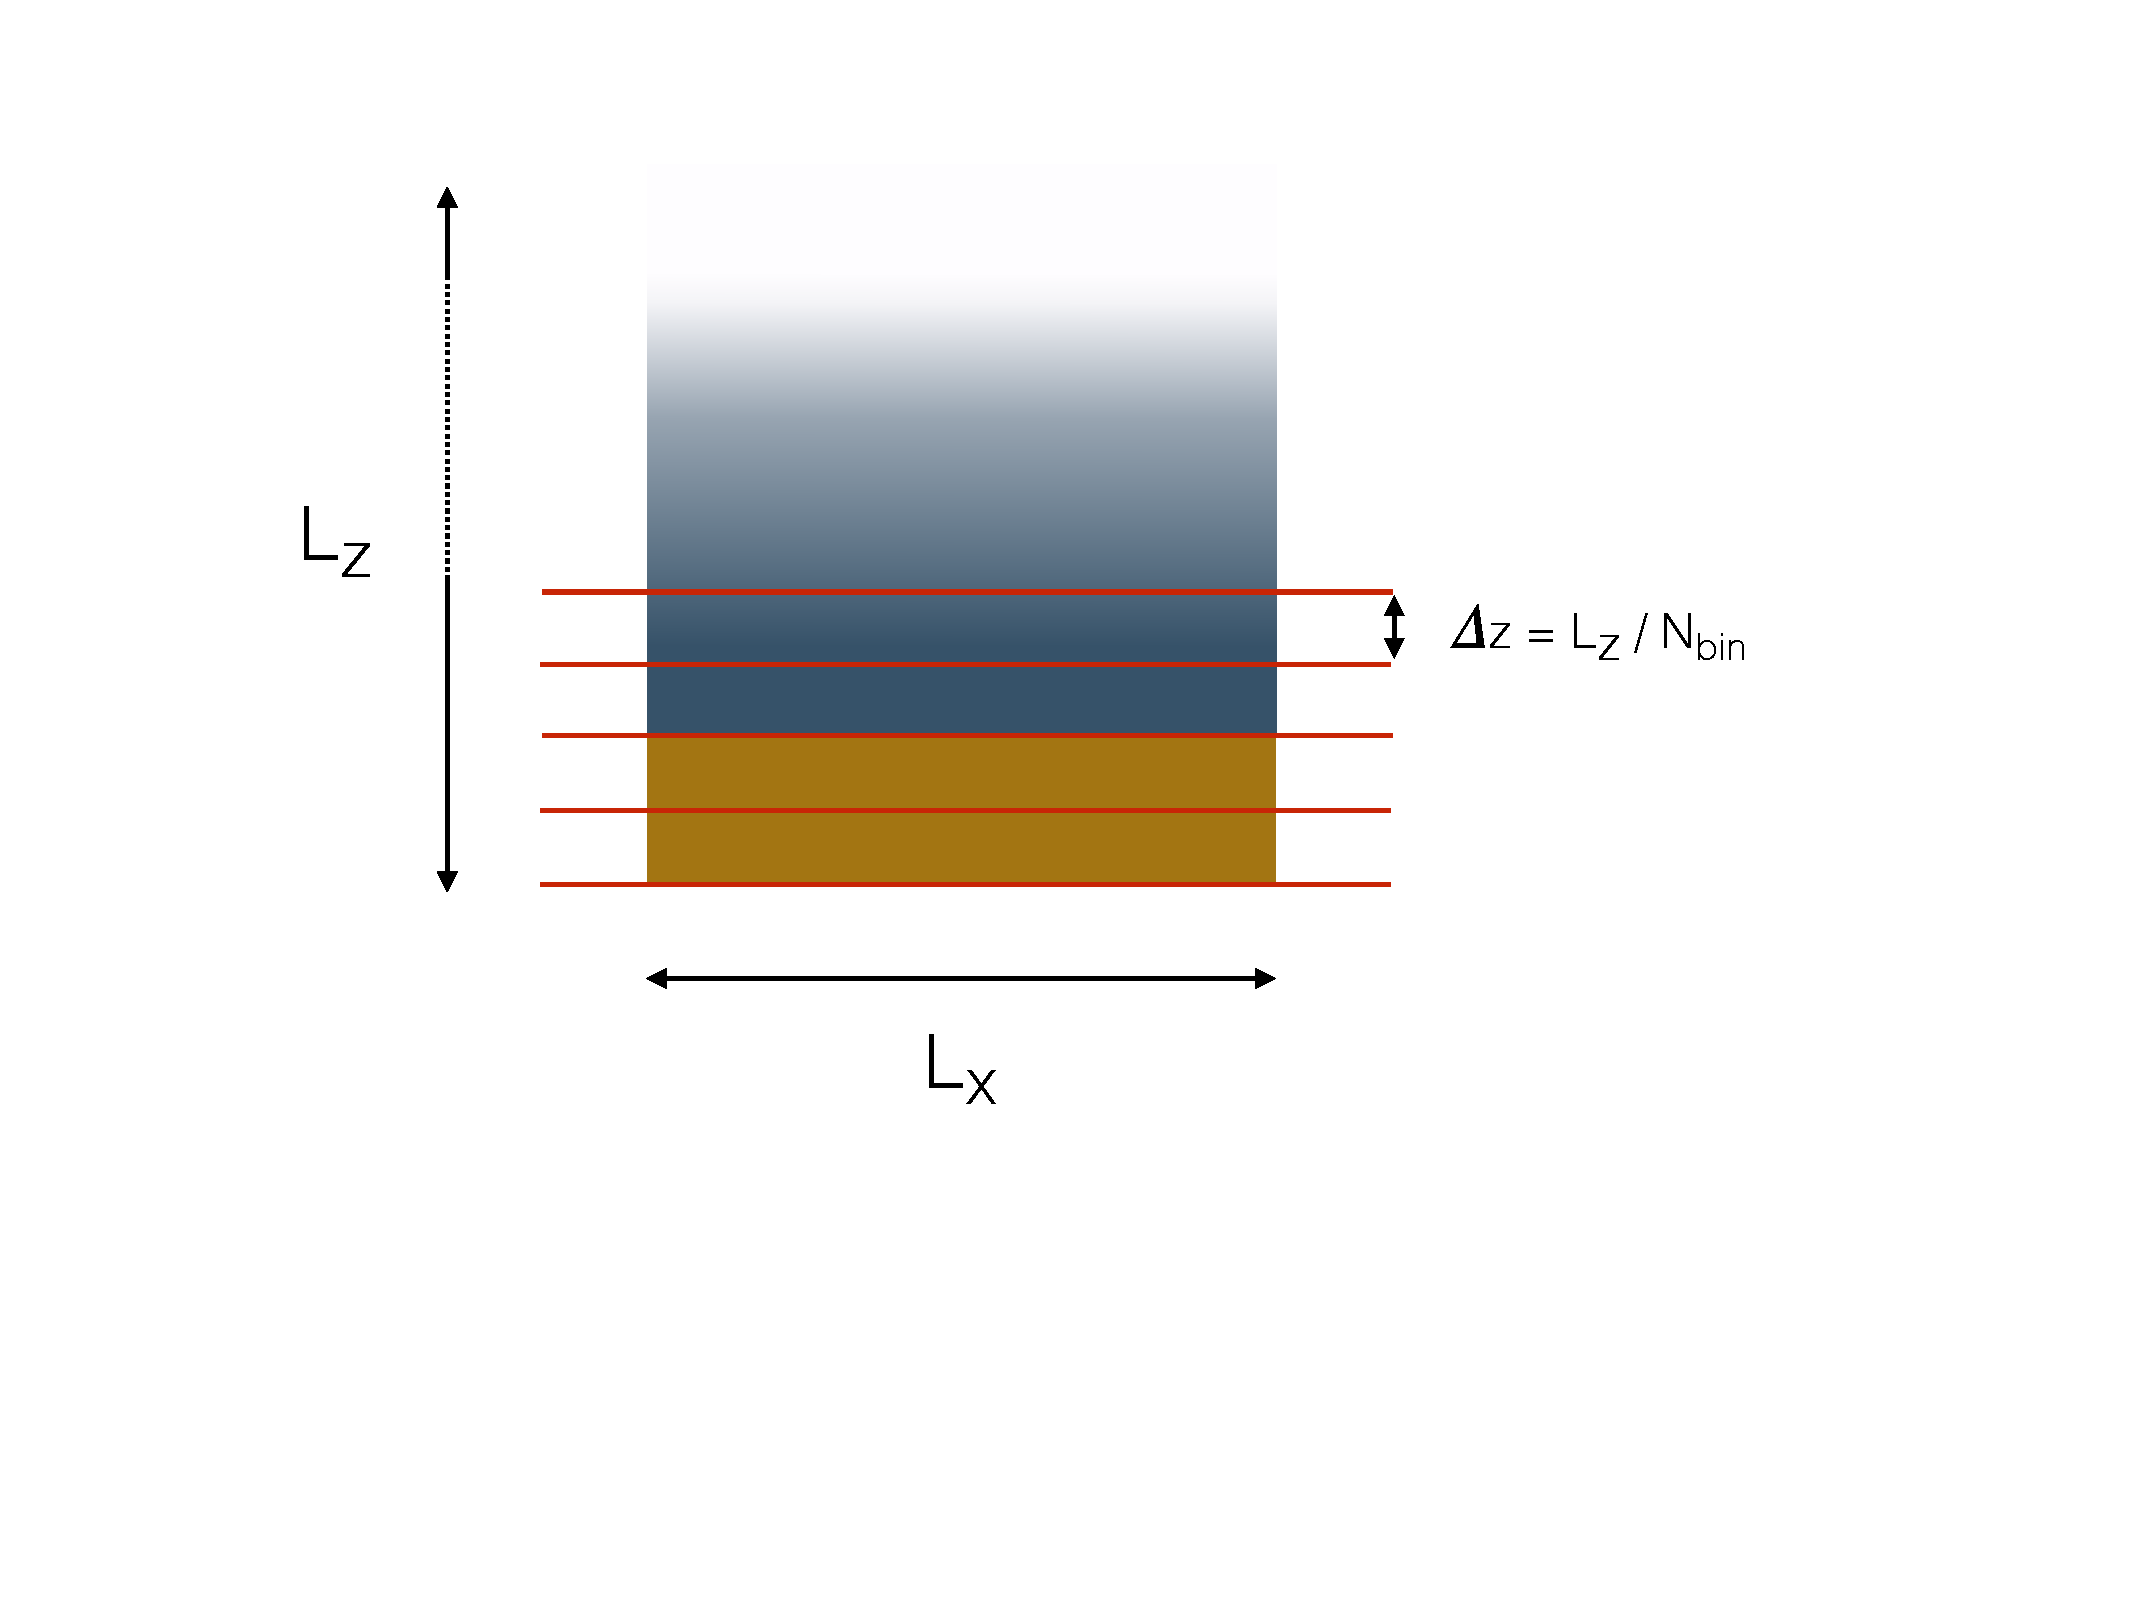
\includegraphics[width=\linewidth]{discrete}
      \end{center}
  \end{frame}

\begin{frame}{Discretización}
  \begin{itemize}
    \item<1-> Función base de elemento finito $\Phi_{\mu}(z)$
  %Función característica $\chi_{\mu}({\bf r})$ y la función base de elemento finito $\Phi_{\mu}({\bf r})$
%    \begin{align}
%    \chi_\mu({\bf r})&=\theta(z_{\mu+ 1}-z)\theta(z-z_\mu)=\chi_\mu(z)
%    \nonumber
%    \end{align}
%    \begin{align}
%      \Phi_\mu({\bf r})=\chi_\mu(z)\frac{z_{\mu+1}-z}{\Delta z}+\chi_{\mu-1}(z)\frac{z-z_{\mu-1}}{\Delta z}
%      \nonumber
%    \end{align}
    \begin{center} 
      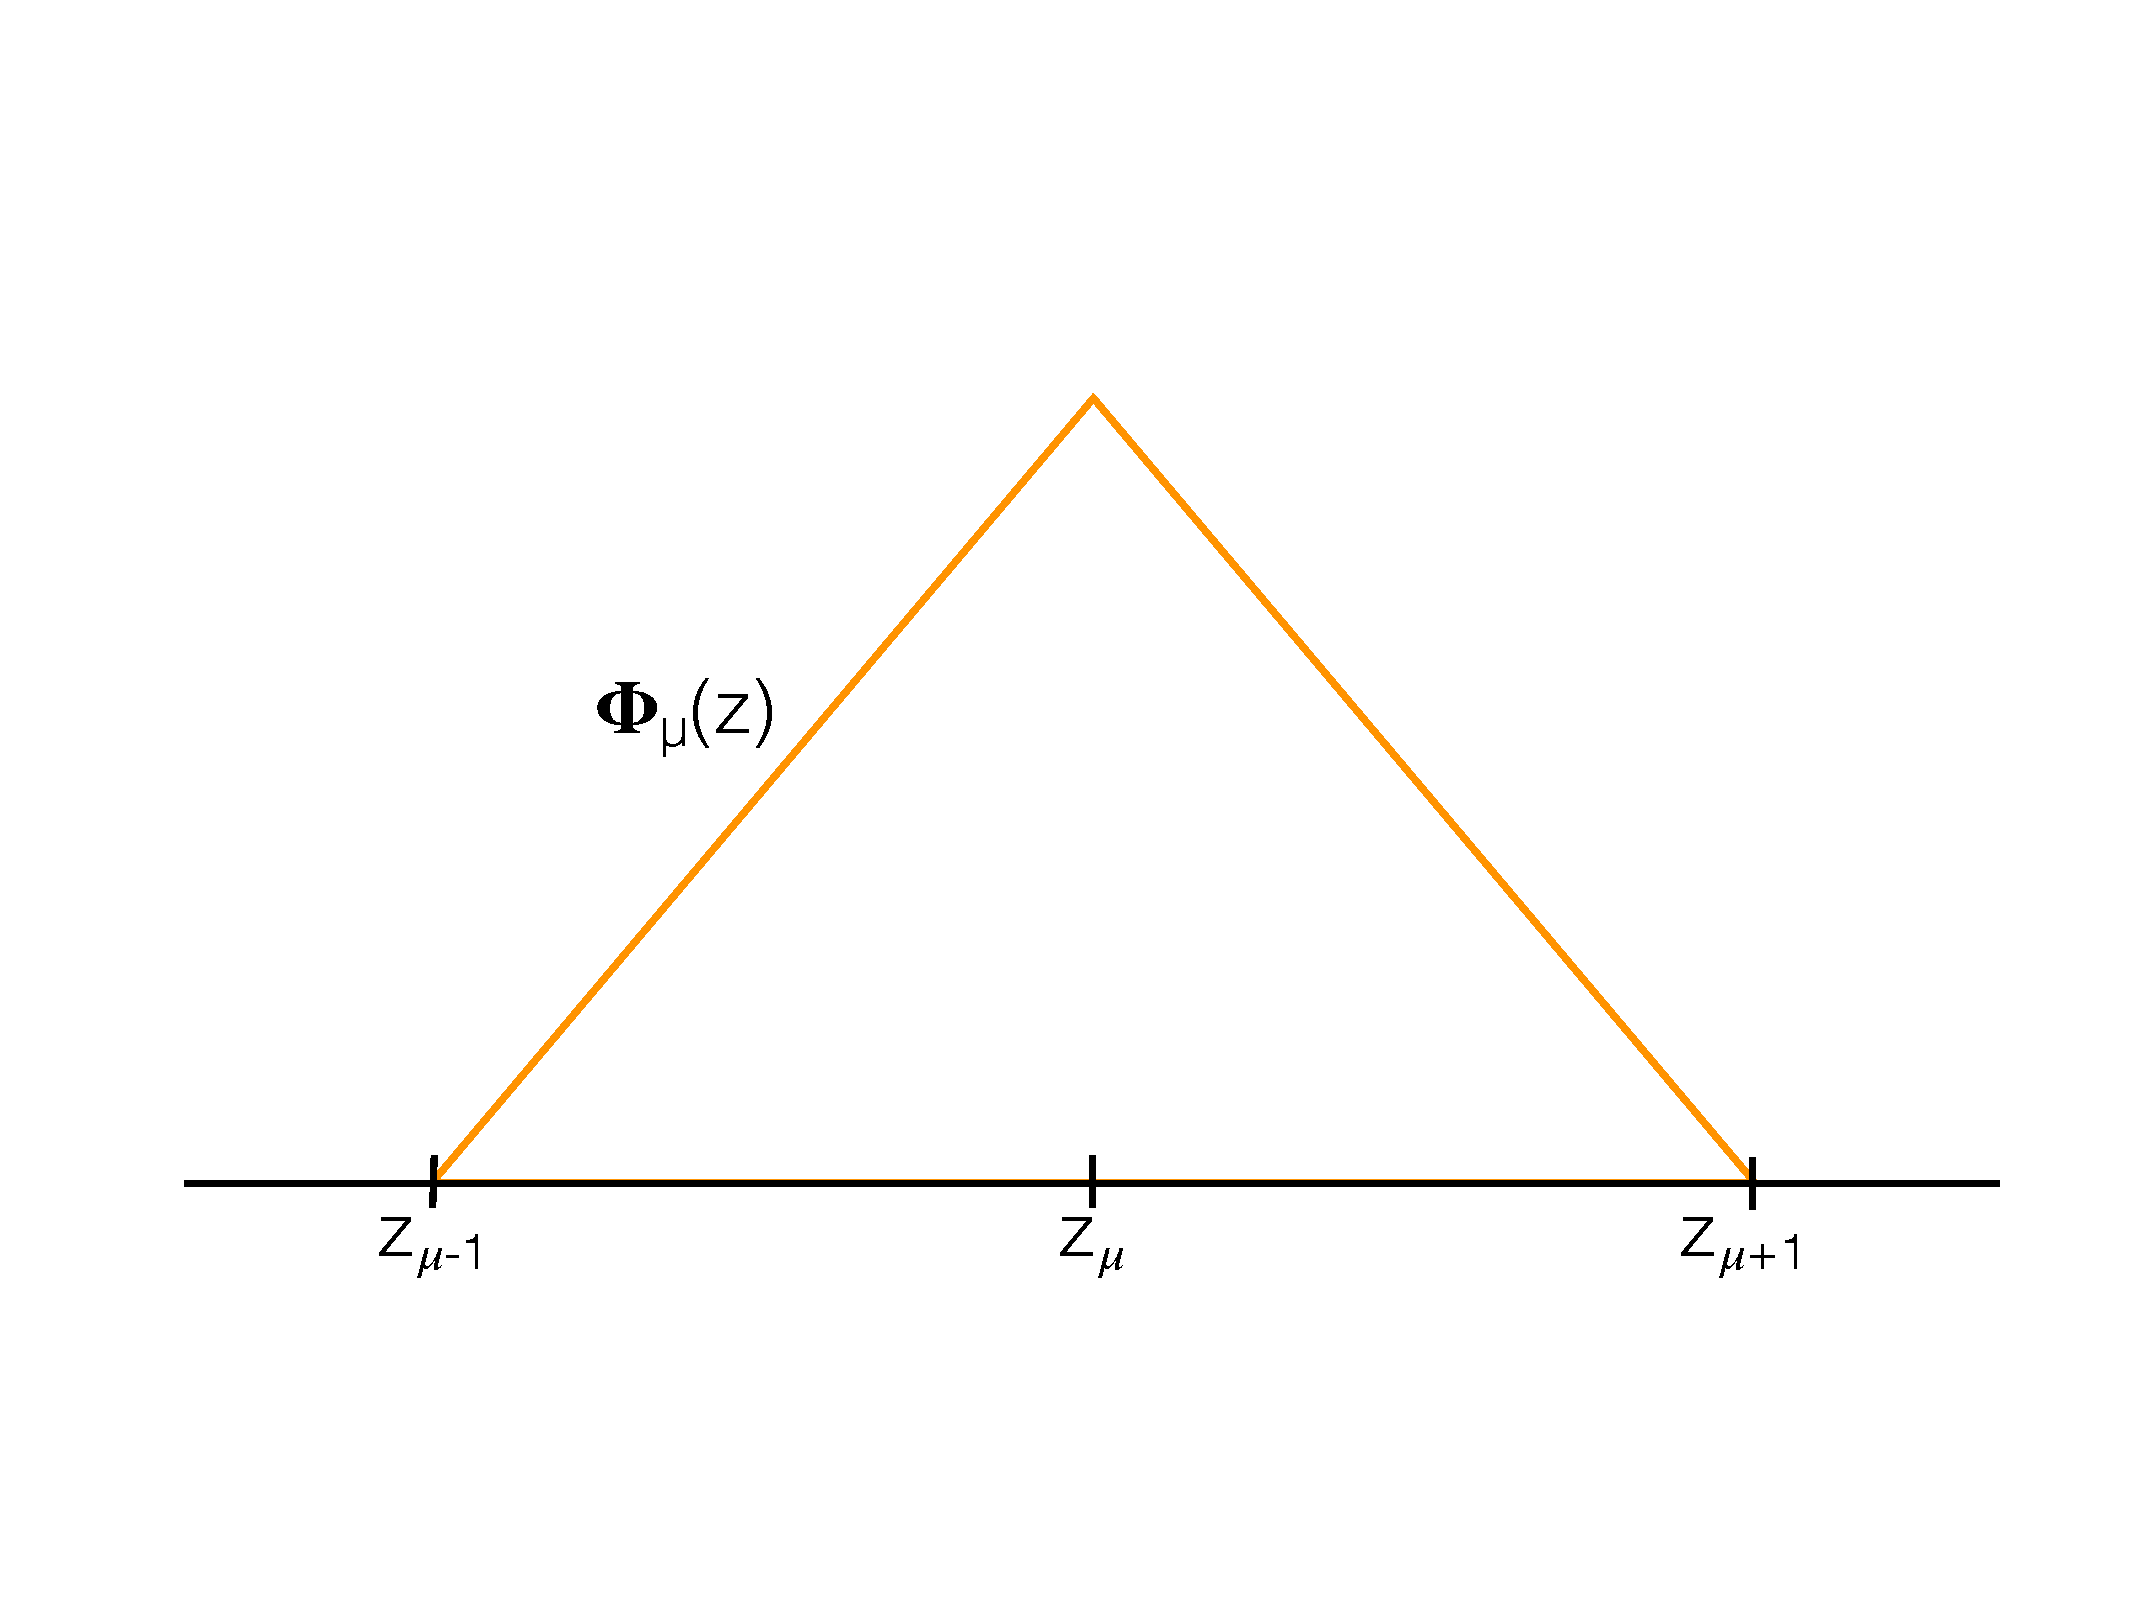
\includegraphics[width = 0.5\linewidth]{psichi-defensa}
      %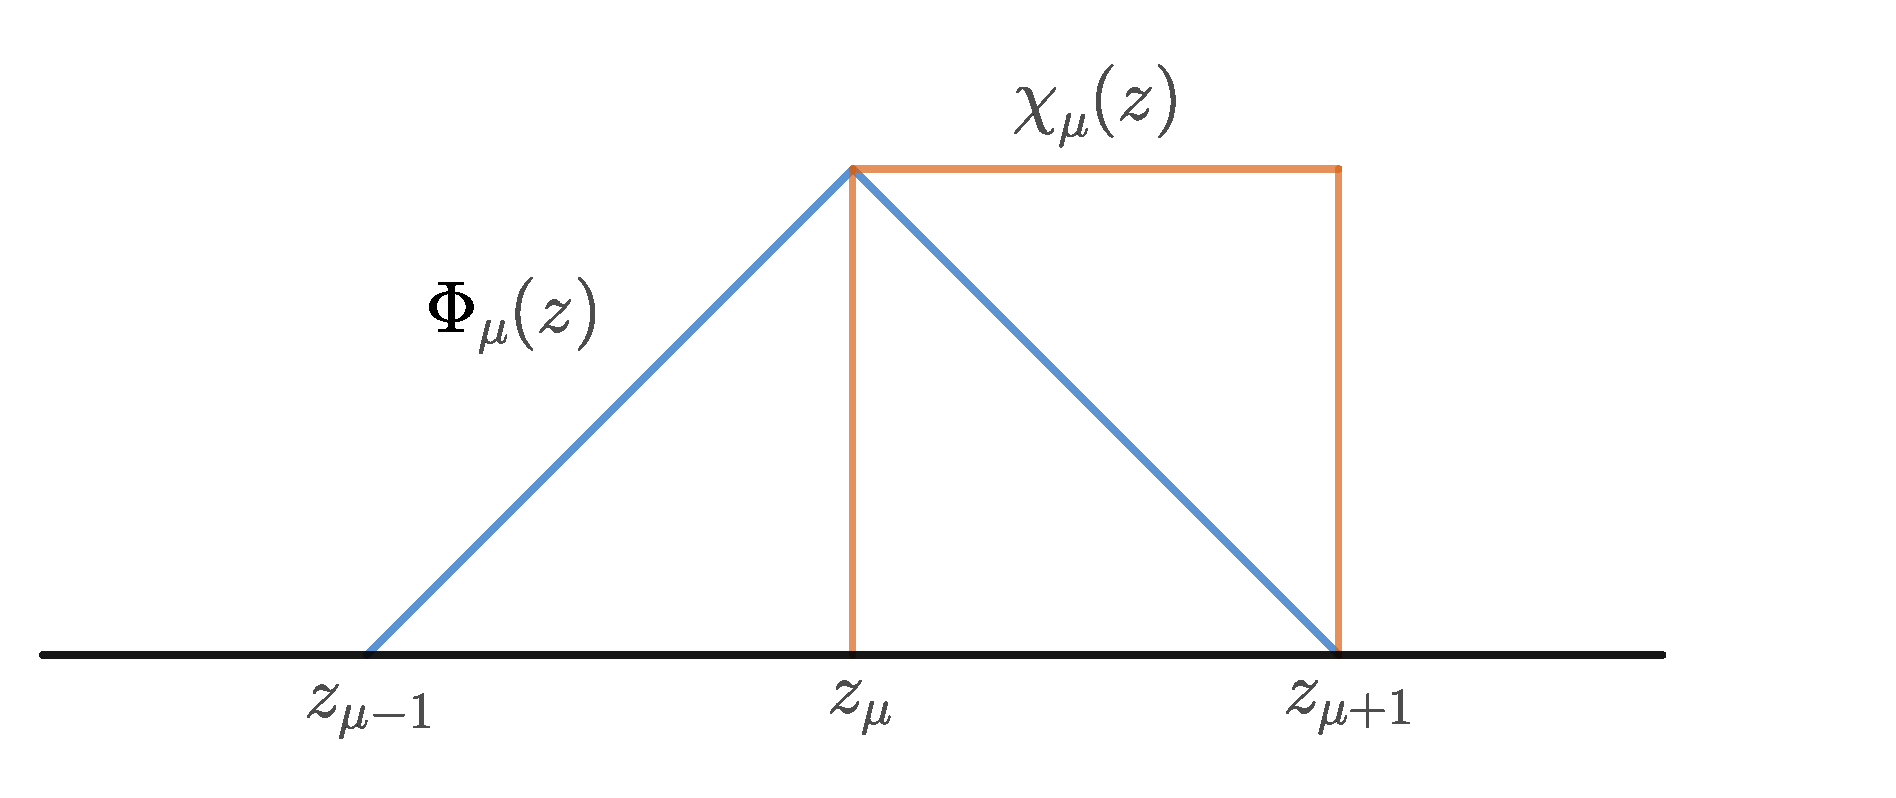
\includegraphics[scale=0.16]{psichi}
    \end{center}
  %\end{itemize}
  \item<2-> Variables relevantes discretas
\begin{align}
  \hat{\rho}_\mu= \sum_i^Nm_i\delta_\mu({\bf q}_i) &&
%\nonumber\\
\hat{\bf g}_\mu= \sum_i^N{\bf p}_i\delta_\mu({\bf q}_i)
\nonumber
\end{align}
\item<3-> La función de Dirac discreta en términos del elemento finito
  \begin{align}
    \delta_{\mu}({\bf r}) \equiv \frac{\Phi({\bf r})}{{\cal V}}
    \nonumber
  \end{align}
\end{itemize}

\end{frame}

%\begin{frame}{Ecuaciones discretas de la hidrodinámica}
%\begin{align}
%  %\frac{d}{dt}\rho_\mu&=  {\color{blue} \llg\overline{\rho} \; \overline{\bf v}\boldsymbol{\nabla}\delta_\mu \rlg}
%  \frac{d}{dt}\rho_\mu&=  {\color{blue} \int d{\bf r}\overline{\rho} \; \overline{\bf v}\boldsymbol{\nabla}\delta_\mu }
%\nonumber\\
%\frac{d}{dt}{\bf g}_\mu&=
%%{\color{blue} \llg\overline{\rho} \overline{\bf v}\;\overline{\bf v}\esc\boldsymbol{\nabla}\delta_{\mu}\rlg
%  {\color{blue} \int d{\bf r}\overline{\rho} \overline{\bf v}\;\overline{\bf v}\esc\boldsymbol{\nabla}\delta_{\mu}
%%-\sum_\nu\llg\overline{\rho}\delta_{\mu}\boldsymbol{\nabla}\delta_{\nu}\rlg
%%\frac{\partial  F}{\partial \rho_{\nu}}(\rho)}
%  -\sum_\nu\int d{\bf r}\overline{\rho}\delta_{\mu}\boldsymbol{\nabla}\delta_{\nu}
%\frac{\partial  F}{\partial \rho_{\nu}}(\rho)}
%\nonumber\\
%&{\color{red}-\sum_{\nu}{\cal V}_\nu \frac{{\bf n}\esc\left[\boldsymbol{\eta}_{\mu\nu}-\boldsymbol{\eta}_{\mu-1\nu}-\boldsymbol{\eta}_{\mu\nu-1}+\boldsymbol{\eta}_{\mu-1\nu-1}\right]}{\Delta z^2}:{\bf n}\tilde{\bf v}_\nu}
%\nonumber\\
%&{\color{red}+\sum_{\nu}{\cal V}_\nu\frac{\left[{\bf G}_{\mu\nu}-{\bf G}_{\mu\nu-1}\right]}{\Delta z}\esc{\bf n}\tilde{\bf v}_\nu}
%\nonumber\\
%&{\color{red}+\sum_{\nu}{\cal V}_\nu\frac{{\bf n}\esc\left[{\bf H}_{\mu\nu}-{\bf H}_{\mu-1\nu}\right]}{\Delta z}\esc\tilde{\bf v}_\nu}
%\nonumber\\
%&{\color{red}-\sum_{\nu}{\cal V}_\nu\boldsymbol{\gamma}_{\mu\nu}\esc\tilde{\bf v}_\nu}
%\nonumber
%\end{align}
%\end{frame}

%\begin{frame}{Una teoría más simple}
%  \begin{itemize}
%    \item<1-> Necesitaríamos obtener demasiada información para calcular las ecuaciones de la hidrodinámica 
%      \begin{itemize}
%        \item $\boldsymbol{\eta}$: 36 componentes independientes.
%        \item ${\bf G}$ y ${\bf H}$: 21 componentes independientes. 
%        \item $\boldsymbol{\gamma}$: 9 componentes independientes.  
%      \end{itemize}
%    \item<2-> Simplificacipnes 
%      \begin{enumerate}
%        \item Paredes planas. 
%        \item Flujos planos. 
%      \end{enumerate}
%    \item<3-> $\rightarrow$ Podemos separar la evolución de las variables relevantes en dos contribuciones: normal y paralela. 
%    \end{itemize}
%\end{frame}

\begin{frame}{Ecs. hidrodinámica: contribución normal y paralela}
\begin{itemize}
  \item<1-> Evolución normal 
\begin{align}
  \frac{d}{dt}\rho_\mu=&  {\color{blue} \llg\overline{\rho} \; \overline{v}^{z}{\nabla}^{z}\delta_\mu \rlg} 
  \nonumber \\
    \frac{d}{dt}{{\bf g}}^{z}_\mu=&
{\color{blue} \llg\overline{\rho}\; \overline{v}^{z}\;\overline{v}^{z}{\nabla}^{z}\delta_{\mu}\rlg
-\llg\overline{\rho}\delta_{\mu}{\nabla}^{z}\delta_{\nu}\rlg
\frac{\partial  F}{\partial \rho_{\nu}}(\rho)}
{\color{red} +M_{\mu\nu}^{\bot}{\cal V}_\nu\tilde{v}^{z}_\nu}
\nonumber
\end{align}
  \item<2-> Evolución paralela 
\begin{align}
  \frac{d}{dt}{{\bf g}}^x_\mu=&{\color{red}-M_{\mu\nu}^{||}{\cal V}_\nu\tilde{v}^x_\nu}
\nonumber
\end{align}
\item<3-> La matriz de fricción para $\odot=||,\bot$
\begin{align}
M^{\odot}_{\mu\nu} 
=&-\frac{\eta^{\odot}_{\mu\nu}-\eta^{\odot}_{\mu-1\nu}-\eta^{\odot}_{\mu\nu-1}+\eta^{\odot}_{\mu-1\nu-1}}{\Delta z^2}
+\frac{{G}^{\odot}_{\mu\nu}-{G}^{\odot}_{\mu\nu-1}}{\Delta z} \nonumber \\
&+\frac{{H}^{\odot}_{\mu\nu}-{H}^{\odot}_{\mu-1\nu}}{\Delta z}
-{\gamma}^{\odot}_{\mu\nu}
\nonumber
\end{align}
\end{itemize}
\end{frame}

\begin{frame}{Versión discreta de los kernels de transporte}
\begin{align}
\eta^{||}_{\mu\nu}&
=\frac{1}{k_BT}\int_0^\tau  dt\left\langle 
{\cal Q}\hat{\boldsymbol{\sigma}}^{xz}_\mu(t){\cal Q}\hat{\boldsymbol{\sigma}}^{xz}_\nu
  \right\rangle^{\lambda(t)}&&
%\nonumber\\
%  {\color{gray} \eta^{\bot}_{\mu\nu}
%= \frac{1}{k_BT}\int_0^\tau  dt\langle 
%{\cal Q}\hat{\boldsymbol{\sigma}}^{zz}_\mu(t)
%  {\cal Q}\hat{\boldsymbol{\sigma}}^{zz}_\nu\rangle}
\nonumber\\
G^{||}_{\mu\nu}&
=\frac{1}{k_BT} \int_0^\tau  dt
\left\langle{\cal Q}\hat{\bf F}^{x}_\mu(t)
{\cal Q}\hat{\boldsymbol{\sigma}}^{xz}_\nu
\right\rangle^{\lambda(t)}&&
%\nonumber\\
%{\color{gray}G^{\bot}_{\mu\nu}=\frac{1}{k_BT} \int_0^\tau  dt
%\left\langle {\cal Q}\hat{\bf F}^{z}_\mu(t)
%{\cal Q}\hat{\boldsymbol{\sigma}}^{zz}_\nu
%  \right\rangle}
\nonumber\\
H^{||}_{\mu\nu}&
=\frac{1}{k_BT} 
\int_0^\tau  dt
\left\langle{\cal Q}\hat{\boldsymbol{\sigma}}^{xz}_\mu(t){\cal Q}\hat{\bf F}^{x}_\nu\right\rangle^{\lambda(t)}&&
\nonumber\\
%{\color{gray}H^\bot_{\mu\nu}=\frac{1}{k_BT} 
%  \int_0^\tau  dt\left\langle {\cal Q}\hat{\boldsymbol{\sigma}}^{zz}_\mu(t){\cal Q}\hat{\bf F}^{z}_\nu\right\rangle}
%\nonumber\\
\gamma^{||}_{\mu\nu}&=
\frac{1}{k_BT} \int_0^\tau  dt
\left\langle 
{\cal Q}\hat{\bf F}^{x}_\mu(t)
{\cal Q}\hat{\bf F}^{x}_\nu\right\rangle^{\lambda(t)}&&
%\nonumber\\
%{\color{gray}\gamma^{\bot}_{\mu\nu}=
%\frac{1}{k_BT} \int_0^\tau  dt\left\langle 
%  {\cal Q}\hat{\bf F}^{z}_\mu(t){\cal Q}\hat{\bf F}^{z}_\nu
%  \right\rangle}
\nonumber
\end{align}
\end{frame}


\metroset{background=dark}
\begin{frame}
  \begin{itemize}
    \item<1-> \alert{Teoría discreta} para flujos planos confinados entre paredes planoparalelas e isotrópicas.
    \item<2-> Nos centraremos en la {componente paralela} del momento   
\begin{align}
  \frac{d}{dt}{{\bf g}}^x_\mu=&-M_{\mu\nu}^{||}{\cal V}_\nu\tilde{v}^x_\nu
\nonumber
\end{align}
    \item<3-> D. Duque-Zumajo, D. Camargo, J. A. de la Torre, F. Chejne, and Pep Espa\~nol. Discrete hydrodynamics for planar flows with confining walls. \textit{Physical Review E}, 2019.
  \end{itemize}

\end{frame}
\metroset{background=white}


\begin{frame}{Kernels de transporte}
\begin{align}
\eta^{||}_{\mu\nu}&
=\frac{1}{k_BT}\int_0^\tau  dt\left\langle 
{\cal Q}\hat{\boldsymbol{\sigma}}^{xz}_\mu(t){\cal Q}\hat{\boldsymbol{\sigma}}^{xz}_\nu
  \right\rangle^{\lambda(t)}&&
%\nonumber\\
%  {\color{gray} \eta^{\bot}_{\mu\nu}
%= \frac{1}{k_BT}\int_0^\tau  dt\langle 
%{\cal Q}\hat{\boldsymbol{\sigma}}^{zz}_\mu(t)
%  {\cal Q}\hat{\boldsymbol{\sigma}}^{zz}_\nu\rangle}
\nonumber\\
G^{||}_{\mu\nu}&
=\frac{1}{k_BT} \int_0^\tau  dt
\left\langle{\cal Q}\hat{\bf F}^{x}_\mu(t)
{\cal Q}\hat{\boldsymbol{\sigma}}^{xz}_\nu
\right\rangle^{\lambda(t)}&&
%\nonumber\\
%{\color{gray}G^{\bot}_{\mu\nu}=\frac{1}{k_BT} \int_0^\tau  dt
%\left\langle {\cal Q}\hat{\bf F}^{z}_\mu(t)
%{\cal Q}\hat{\boldsymbol{\sigma}}^{zz}_\nu
%  \right\rangle}
\nonumber\\
H^{||}_{\mu\nu}&
=\frac{1}{k_BT} 
\int_0^\tau  dt
\left\langle{\cal Q}\hat{\boldsymbol{\sigma}}^{xz}_\mu(t){\cal Q}\hat{\bf F}^{x}_\nu\right\rangle^{\lambda(t)}&&
\nonumber\\
%{\color{gray}H^\bot_{\mu\nu}=\frac{1}{k_BT} 
%  \int_0^\tau  dt\left\langle {\cal Q}\hat{\boldsymbol{\sigma}}^{zz}_\mu(t){\cal Q}\hat{\bf F}^{z}_\nu\right\rangle}
%\nonumber\\
\gamma^{||}_{\mu\nu}&=
\frac{1}{k_BT} \int_0^\tau  dt
\left\langle 
{\cal Q}\hat{\bf F}^{x}_\mu(t)
{\cal Q}\hat{\bf F}^{x}_\nu\right\rangle^{\lambda(t)}&&
%\nonumber\\
%{\color{gray}\gamma^{\bot}_{\mu\nu}=
%\frac{1}{k_BT} \int_0^\tau  dt\left\langle 
%  {\cal Q}\hat{\bf F}^{z}_\mu(t){\cal Q}\hat{\bf F}^{z}_\nu
%  \right\rangle}
\nonumber
\end{align}
\end{frame}


\begin{frame}{Problema del plateau}
\begin{figure}[]
  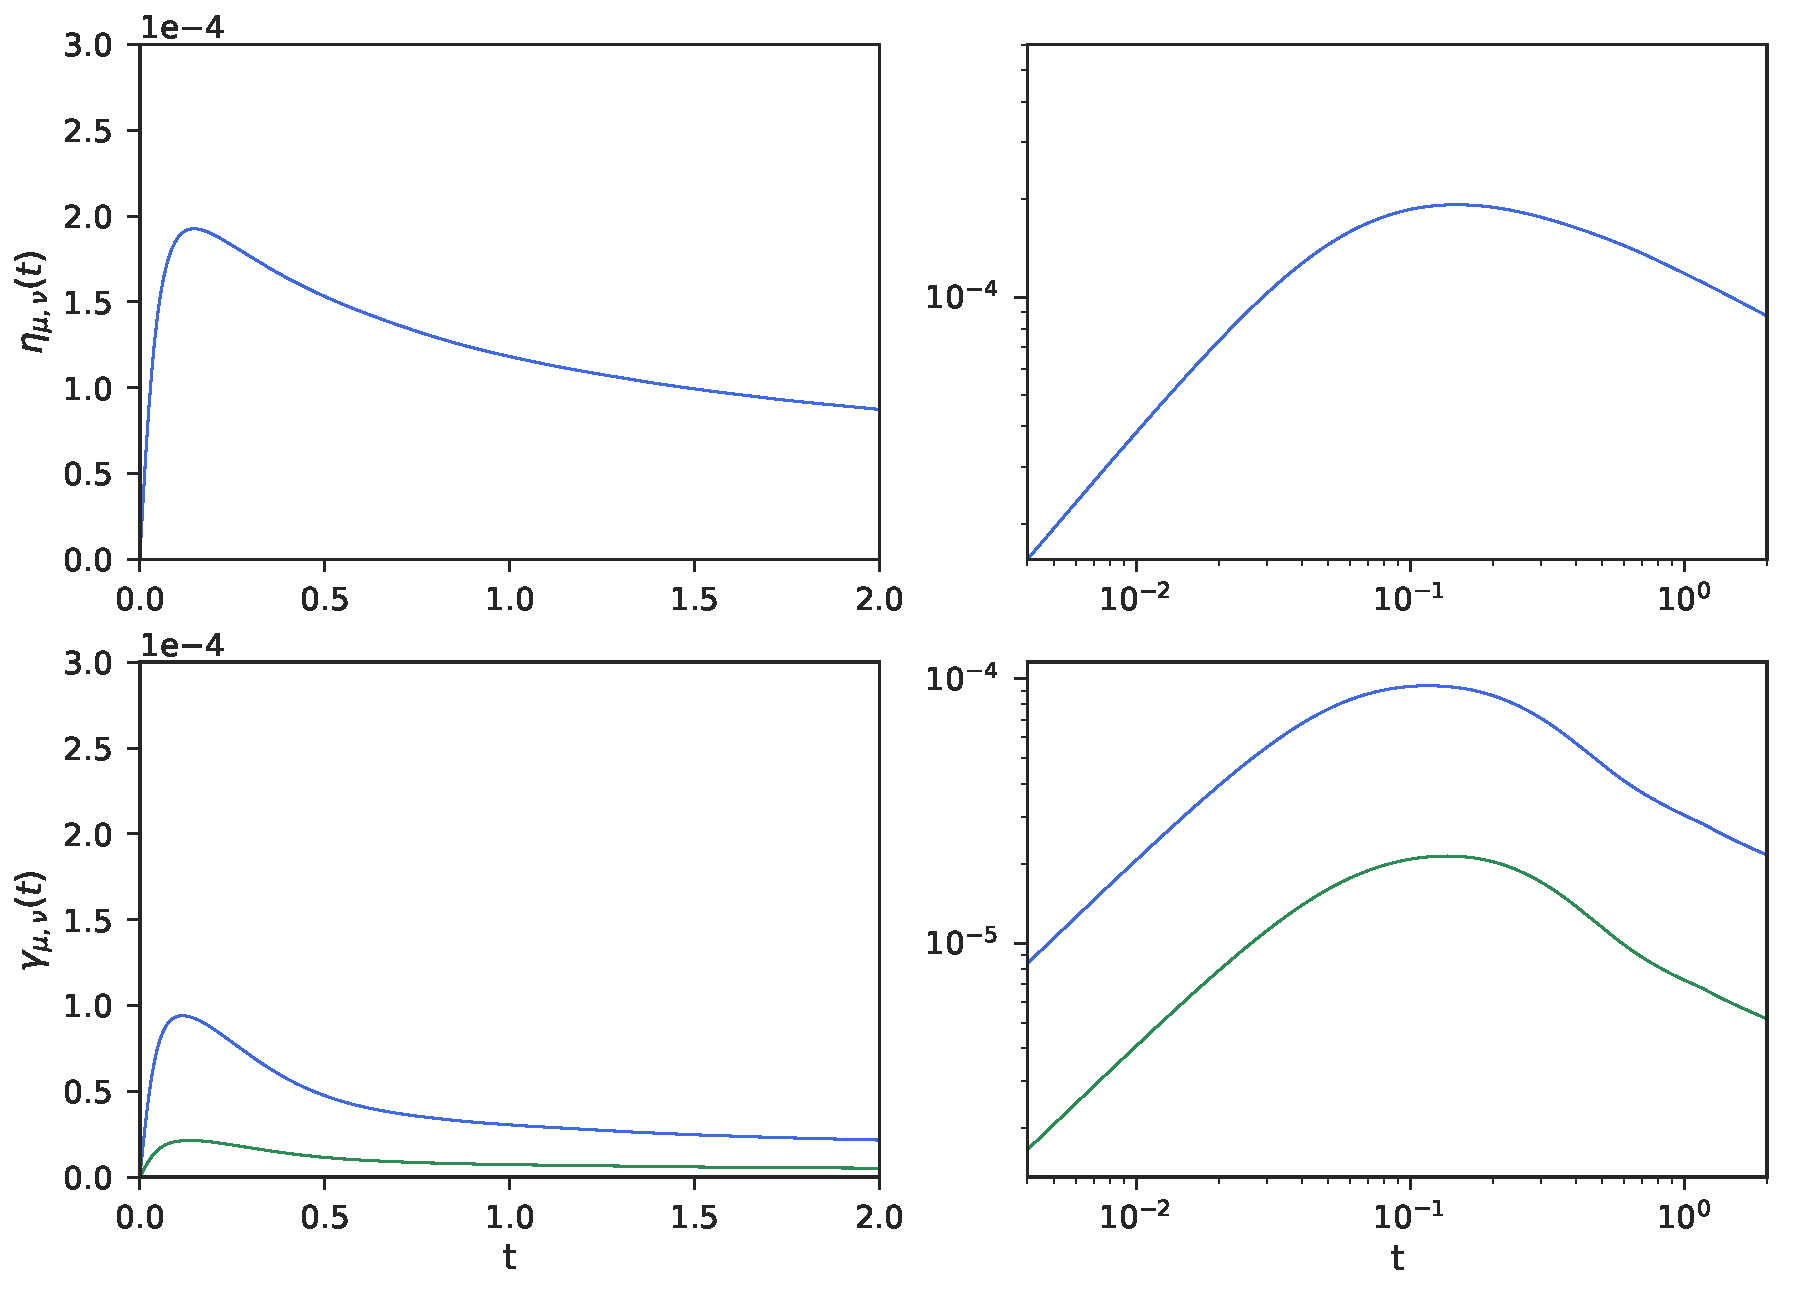
\includegraphics[scale=0.33]{NoPlateau-WALLS-17nodes}
\end{figure}
\end{frame}

%\begin{frame}{Hoja de ruta}
%  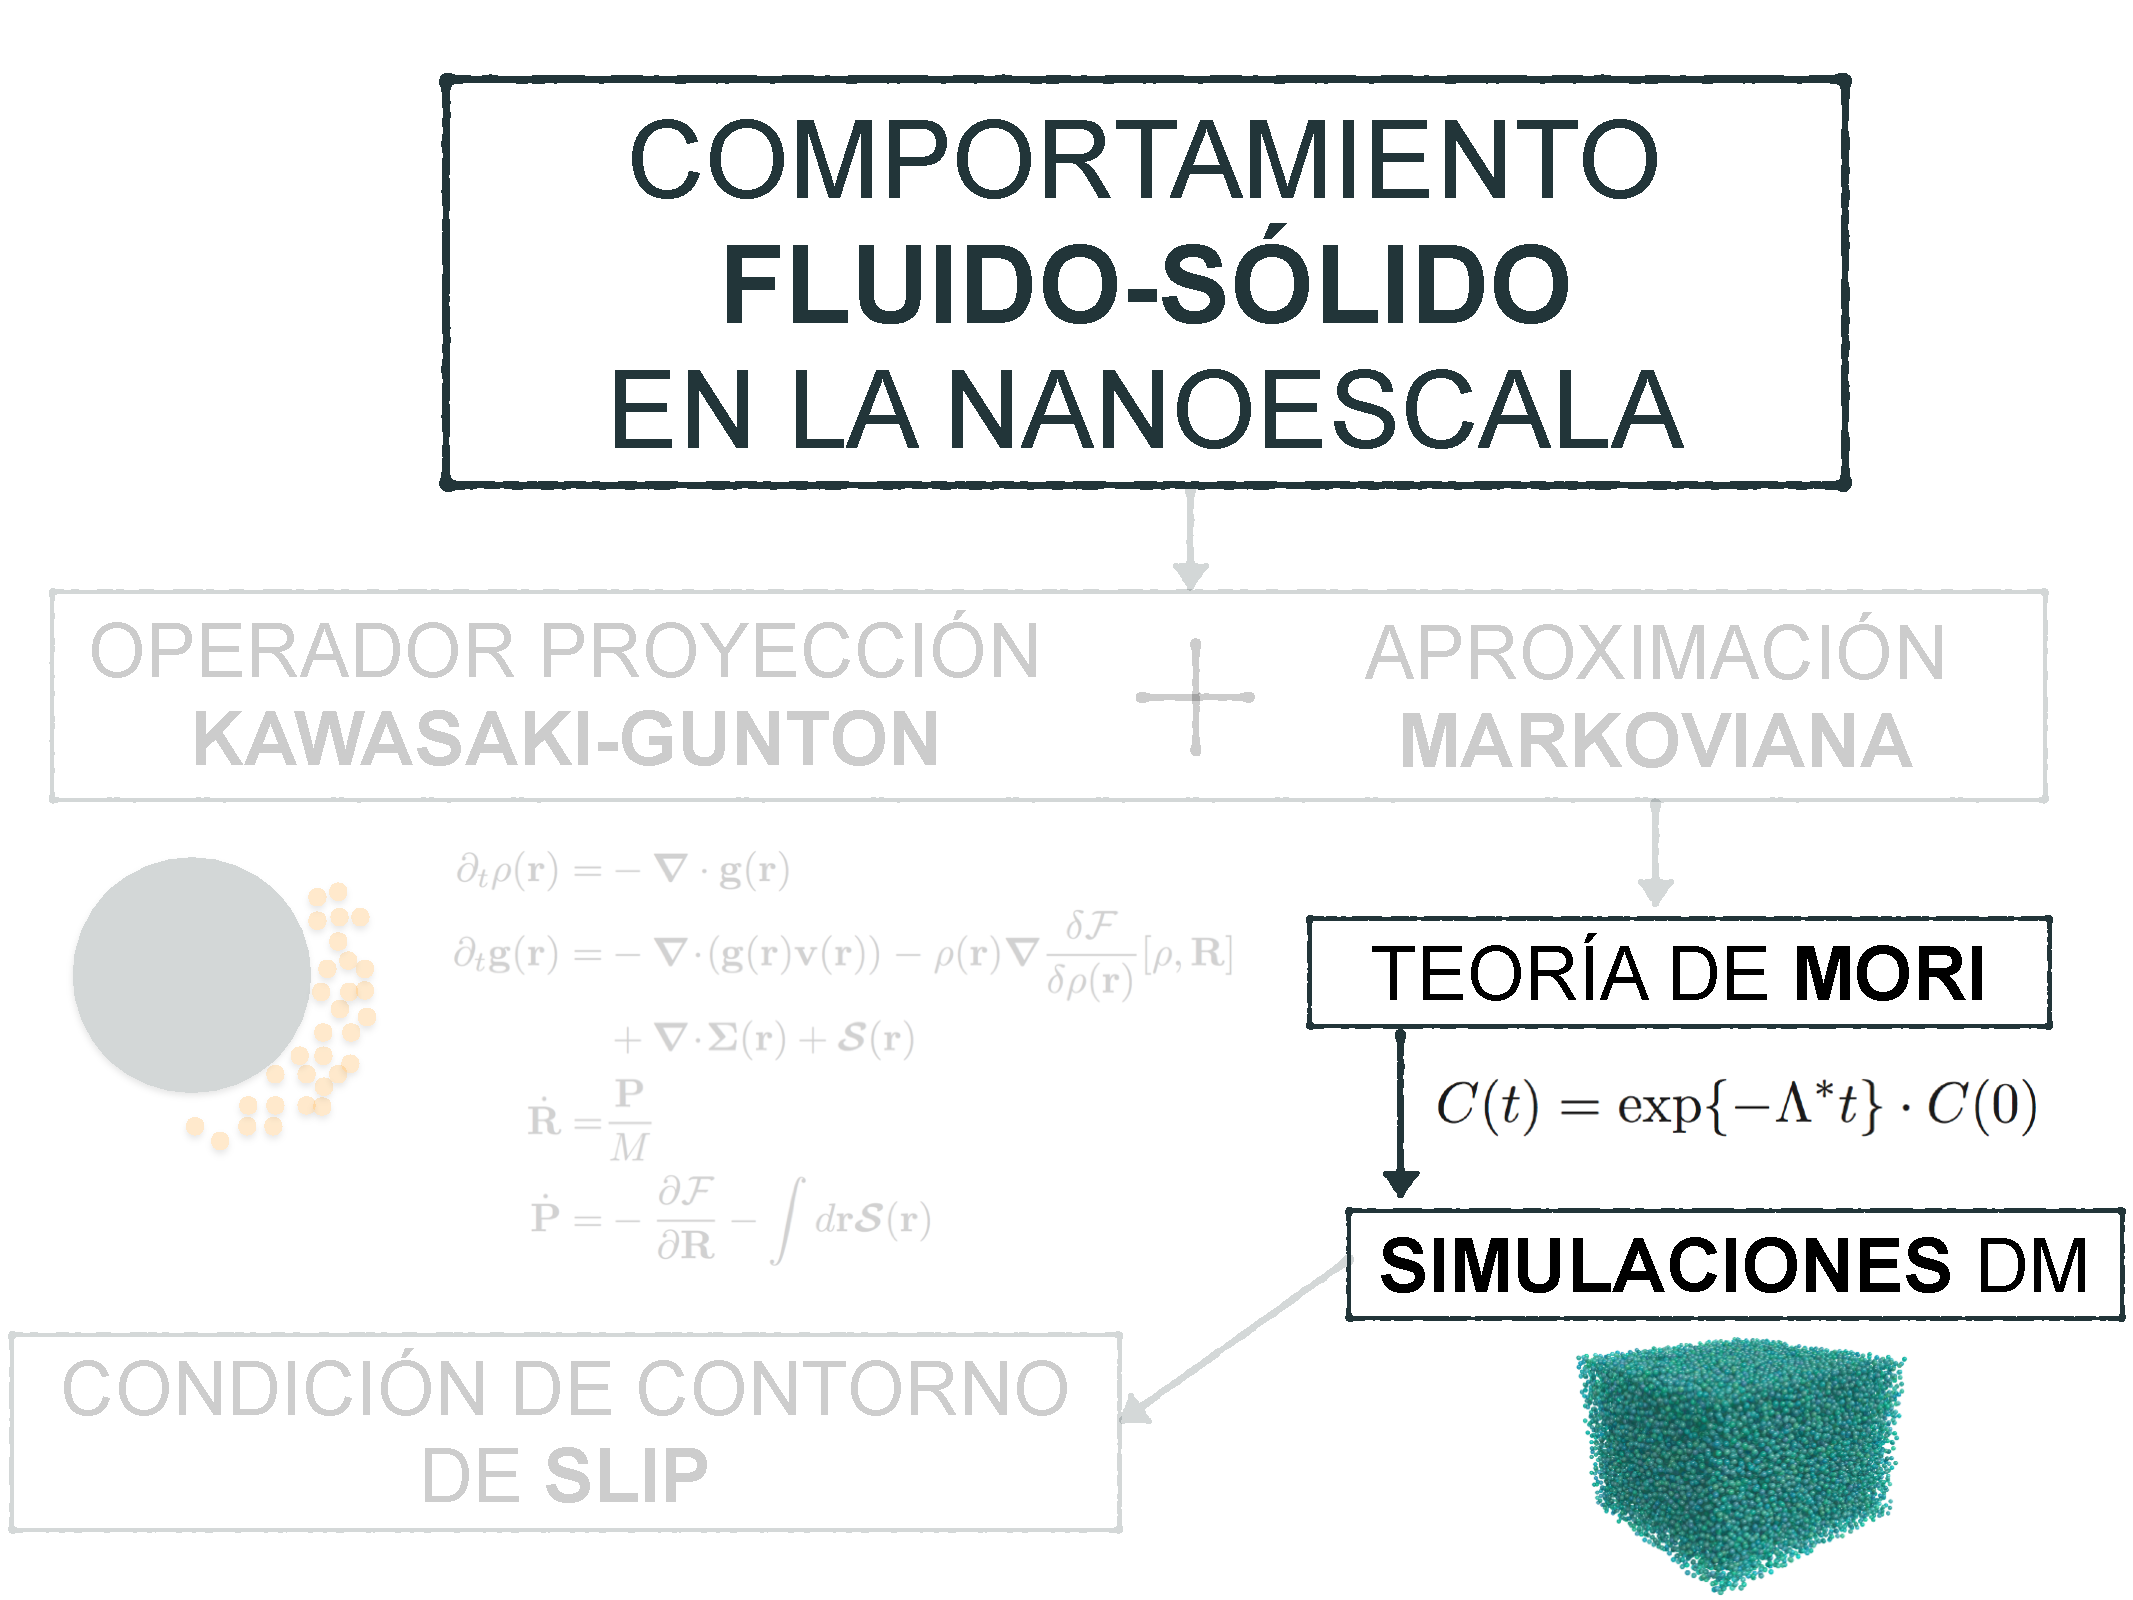
\includegraphics[width=\linewidth]{scheme-thesis-mori}
%\end{frame}

\section{Teoría de Mori}
\begin{frame}{Teoría de Mori}
  \begin{itemize}
    \item<1-> Ecuaciones lineales para las correlaciones de $\hat{A}(t)$
\begin{align}
  \frac{d}{dt}C(t)&=-L\esc C^{-1}(0)\esc C(t)
  -{\color{orange}\int_0^tdt' \Gamma(t-t')\esc C^{-1}(0)\esc  C(t')}
\nonumber
\end{align}
      donde $C(t)=\langle\hat{A}(t)\hat{A}\rangle$ y $L=\langle \hat{A}i{\cal L}\hat{A}^T\rangle$.
%where the following matrices have been introduced
%\begin{align}
%  L&=\langle \hat{A}i{\cal L}\hat{A}^T\rangle \nonumber \\
%  C(0)&=\langle \hat{A}\hat{A}^T\rangle \nonumber \\
%\Gamma(t)&=\langle F^+(t)F^{+T}(0)\rangle
%\nonumber
%\end{align}
%\item<2-> The projected forces are given by
%\begin{align}
%F^+(t)&= \exp\{{\cal Q}i{\cal L}t\} {\cal Q}i{\cal L}\hat{A}  
%\nonumber
%\end{align}
%\item<3-> ${\cal Q}=1-{\cal P}$ where  ${\cal P}$  is Mori's  projector 
%\begin{align}
%  {\cal P}\hat{F}(z) = \langle \hat{F}\rangle+ \langle \hat{F}\hat{A}^T \rangle\esc  C^{-1}(0)\esc  \hat{A}(z)
%\nonumber
%\end{align}
%\end{itemize}
%\end{frame}

%\begin{frame}{aproximación Markoviana}
%  \begin{itemize}
    %\item Memory-less término 
    \item<2-> Aproximación Markoviana
  \begin{align}
{\color{orange}\int_0^tdt' \Gamma(t-t')\esc C^{-1}(0)\esc  C(t')} \simeq M^* C^{-1}(0)C(t)
\nonumber
\end{align}
\item<3-> Ecuación de Mori y aproximación Markoviana
\begin{align}
  \frac{d}{dt}C(t) &= - (L+M^*)\esc C^{-1}(0)\esc C(t) 
                     \equiv -\Lambda^*\esc C(t)
  \nonumber
\end{align}
%\item For a linear Markovian teoría the only posibilidad for a correlación is to decay in an exponential matrix way
\item<4-> \textbf{Decaimiento exponencial}
\begin{align}
  C(t)=\exp\{-\Lambda^* (t-\tau)\}\esc C(\tau)
\nonumber
\end{align}
\item<5-> {\bf Si el comportamiento es Markoviano $\boldsymbol{\Lambda^*}$ es constante}.
\end{itemize}
\end{frame}

\begin{frame}{Simulaciones}
\begin{figure}[!htb]
   \begin{minipage}{0.5\textwidth}
     \centering
     \includegraphics[width=1\linewidth]{temp_wo_walls}
   \end{minipage}\hfill
   \begin{minipage}{0.5\textwidth}
     \centering
     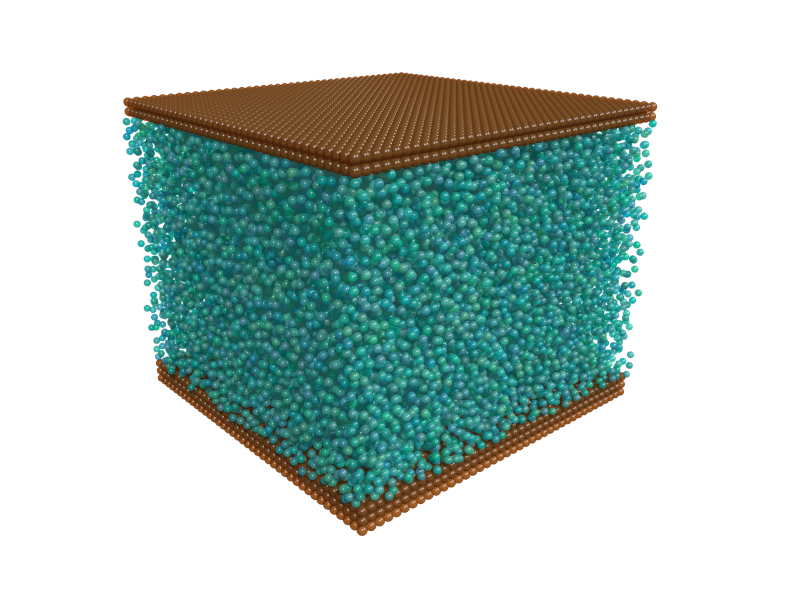
\includegraphics[width=1\linewidth]{PRL3_gold2_wo_layers_wo_diffuse}
   \end{minipage}
\end{figure}
\end{frame}


\section{Estudio de la Markovianidad en fluidos no confinados}
\begin{frame}{Simulaciones fluido no confinado}
  \begin{center}
  %\begin{itemize}
  %\item The sistema
  \begin{figure}
    %\includegraphics[width=0.5\linewidth]{temp_wo_walls}
    %\includegraphics[width=0.5\linewidth]{temp_wo_walls}
    \includegraphics[width=0.5\linewidth]{sim-pbc-box}
%    \includegraphics[width=0.5\linewidth]{temp_wo_walls_w_layers2}
\end{figure}
%\item The relevante variable
%\begin{align}
%  \hat{\bf g}_\mu(z)= \sum_i^N{\bf p}_i\delta_\mu({\bf r}_i)
%%  i{\cal L}  \hat{g}_{\mu}(z)=-\frac{\hat{\sigma}^{xz}_{\mu}-\hat{\sigma}^{xz}_{\mu-1}}{\Delta z}
%\nonumber
%\end{align}
%\end{itemize}
    \begin{itemize}
     \item $28749$ partículas.
     \item Potencial LJ truncado en $2.5\sigma$.
     \item $L_{x}=40\sigma$, $L_{y}=40\sigma$, $L_{z}=30\sigma$.
     %\item $dt=2\cdot 10^{-4}$. 
    \end{itemize}
  \end{center}
\end{frame}


\begin{frame}{Simulaciones fluido no confinado}
  %\begin{figure}
  %  \includegraphics[width=0.5\linewidth]{sim-pbc-box-bin}
  %\end{figure}
   \begin{itemize}
     %\item Simulation of $28749$ particles interacting with a LJ potential truncated at $\sigma=2.5$.
     %\item Box size $40x40x30$.
     \item<1-> Fase de \alert{equilibrado}
       \begin{itemize}
         %\item Termostato durante $10^5$ pasos de tiempo: $T=2.0$, $\rho=0.6$.
         \item Termostato de Langevin: $T=2.0$, $\rho=0.6$.
         %\item NVE durante $10^5$ pasos de tiempo.
         \item Quitamos termostato y dejamos que corra en NVE.
          \end{itemize}
        \item<2-> Fase de \alert{producción}
       \begin{itemize}
         %\item $1.5\times10^6$ pasos de tiempo.
         \item Medición de $g_{\mu}^x(t)$.
           %medido cada $10$ pasos de tiempo.
         \item $z$ discretizado en $60$ bines $\mu$ $\rightarrow$ {$\boldsymbol{\Delta} {\bf z=0.5}\boldsymbol{\sigma}$}.
         \end{itemize}
       \item<2->[]\begin{figure}
    \includegraphics[width=0.5\linewidth]{sim-pbc-box-bin}
  \end{figure}
     \end{itemize}
 \end{frame}

% \begin{frame}{Building the correlación matrix $C(t)$}
%\begin{figure}[h!]
%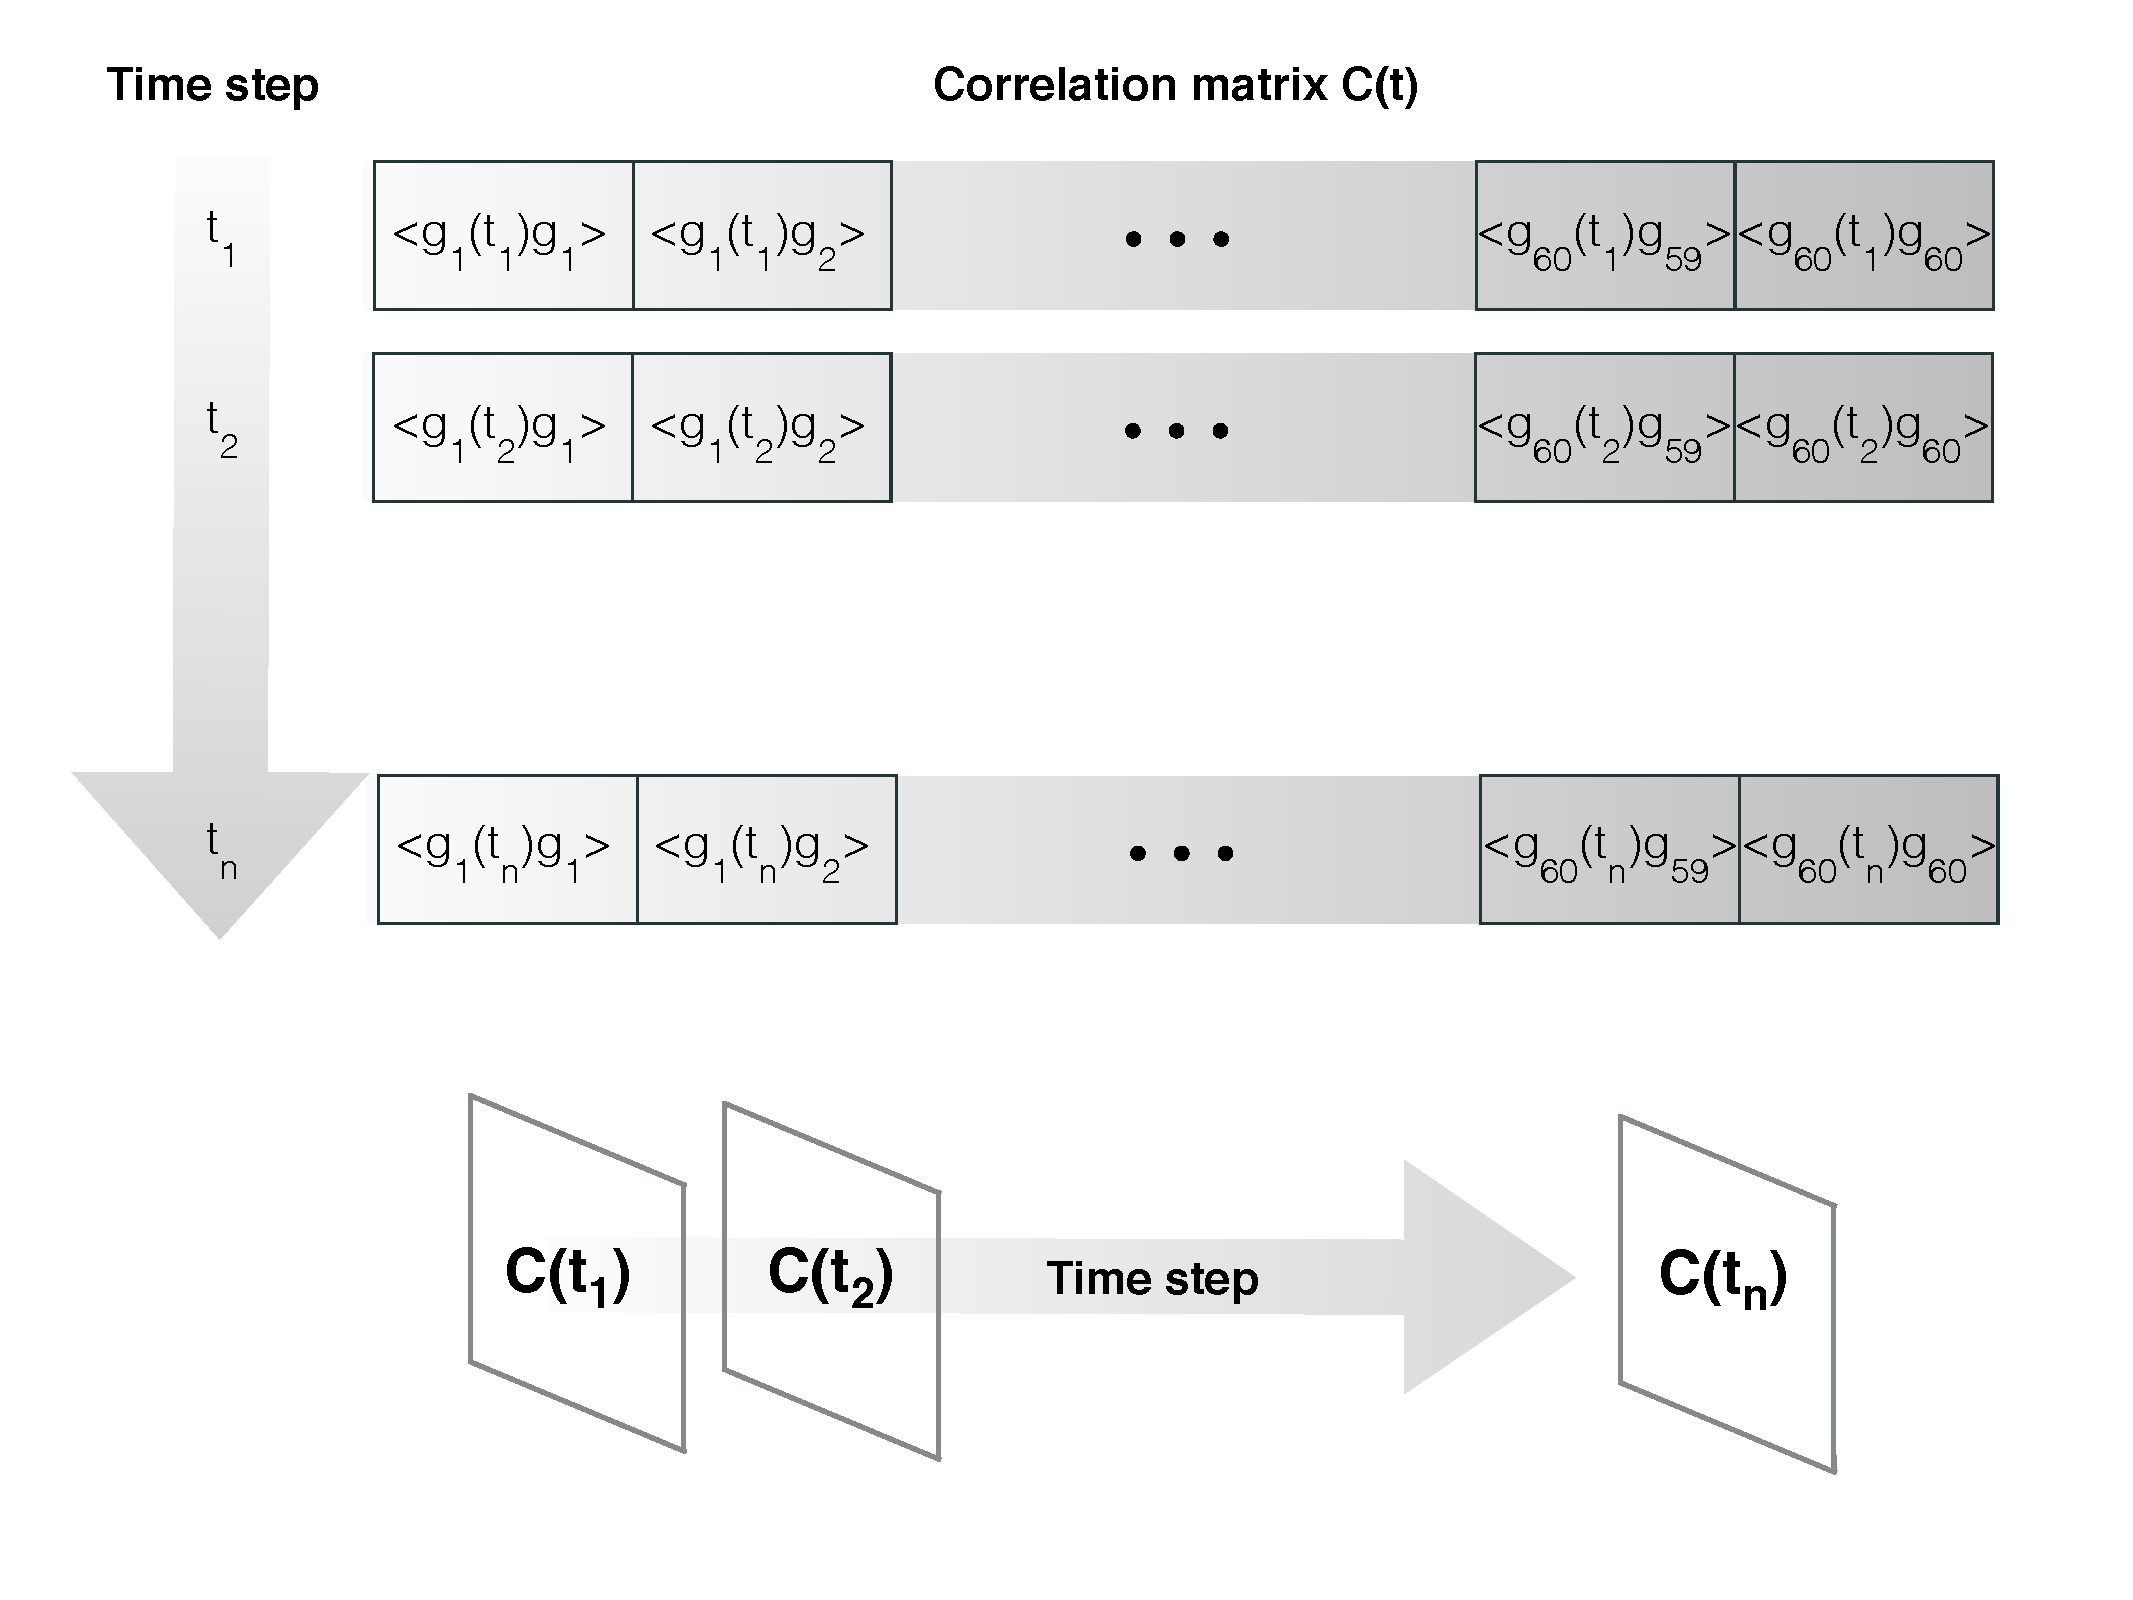
\includegraphics[width=\linewidth]{lammps-python}
%\end{figure}
% \end{frame}

 \begin{frame}{La matriz de correlaciones C(t) y sus autovalores  $\tilde{C}_{\mu\mu}$}
   \begin{itemize}
 \item<1->
   Matriz de correlaciones $C(t)$ en $t=0$ (izq.) y $t=0.6$ (dcha.)
\begin{figure}[h!]
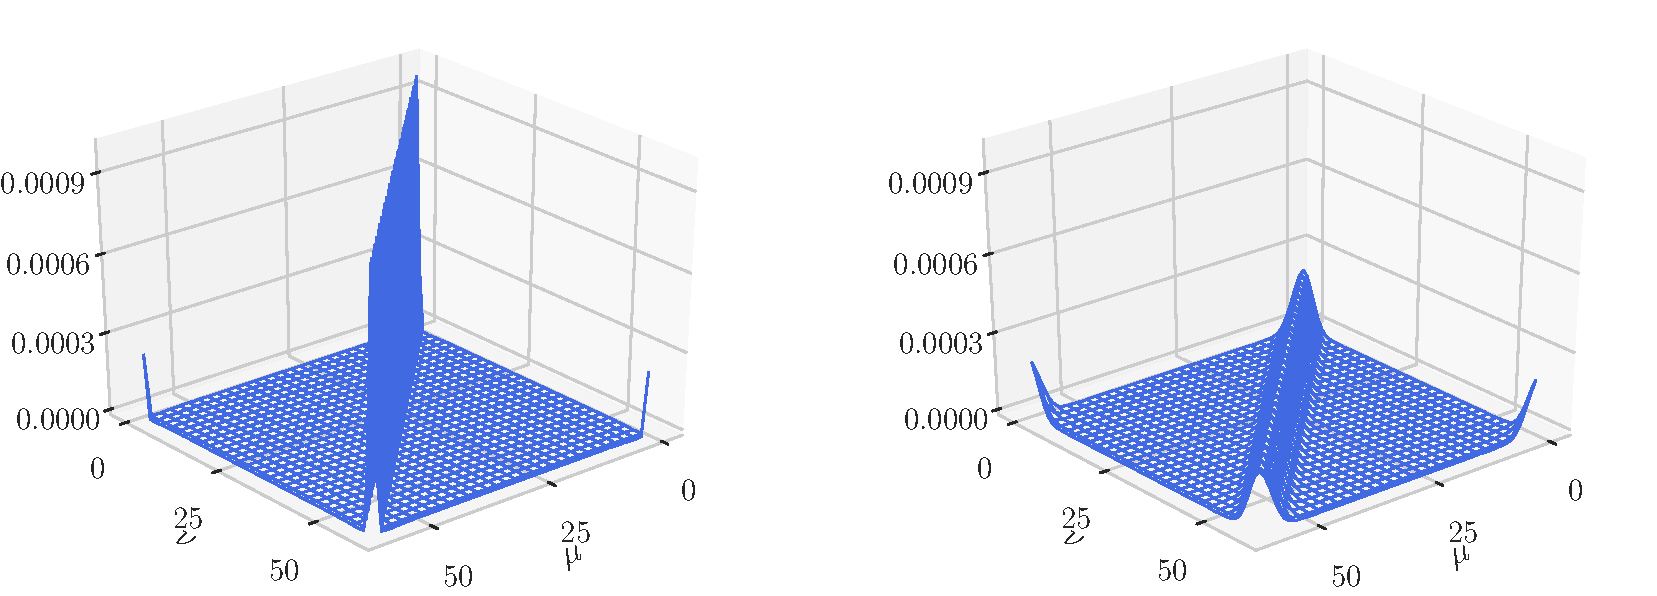
\includegraphics[width=\linewidth]{Ct-matrix-PBC}
\end{figure}
\item<2->  Evolución de los distintos autovalores $\tilde{C}_{\mu\mu}(t)$. %The horizontal  line  at  the   value  $2\times10^{-5}$,  signaling  the
  %threshold below which statistical errors give spurious results.
\begin{figure}[h!]
  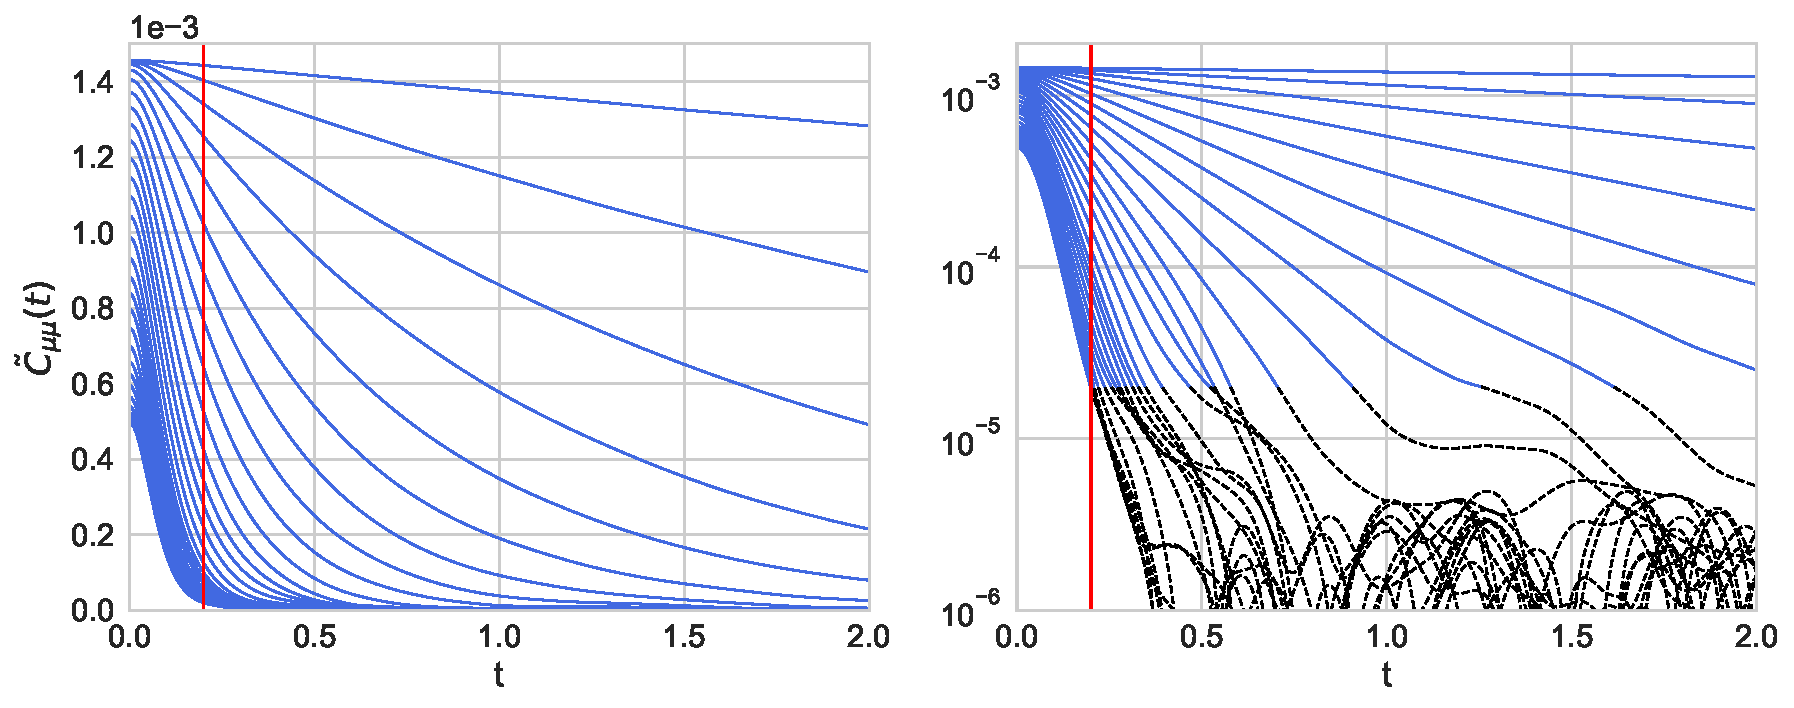
\includegraphics[width=\linewidth]{CtFourier-PBC-exp}
\end{figure}
\end{itemize}
\end{frame}

\begin{frame}{Validación de la aproximación Markoviana}
\begin{align}
  \tilde{\Lambda}_{\mu\mu}=-\frac{1}{\tilde{C}_{\mu\mu}(t)}\frac{d\tilde{C}_{\mu\mu}}{dt}(t)
  \nonumber
\end{align}
\begin{figure}[h!]
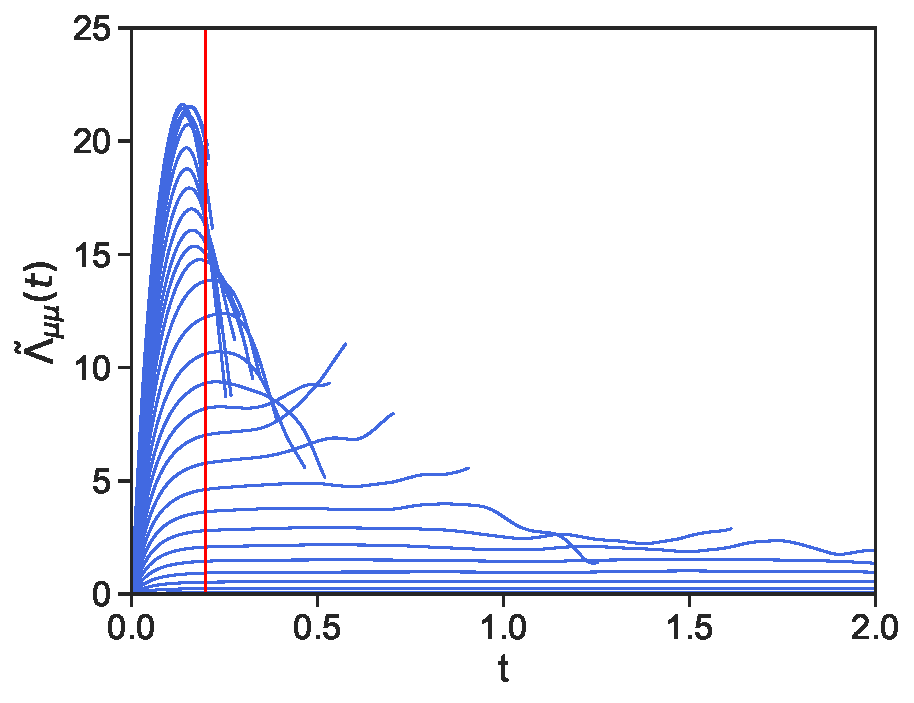
\includegraphics[width=0.7\linewidth]{LambdatFourier-PBC-defense}
\end{figure}
%  Left:
%  in ascending  order times  go  from $t=0$  to $t=0.20$  in
%  intervals of $0.02$.  Right: time evolution of $\tilde{\Lambda}_{\mu\mu}(t)$.
\end{frame}

\metroset{background=dark}
\begin{frame}
  \begin{itemize}
    \item<1-> Para estudiar la validez de la aproximación Markoviana es conveniente hacerlo en el \alert{espacio recíproco} (Fourier para un fluido en PBC). 
    \item<2-> Observamos una \alert{matriz $\tilde{\Lambda}$ constante} a partir de un tiempo $\tau=0.2$ para la mayoría de los modos.  
    \item<3-> Las predicciones de la matriz de correlaciones con la teoría Markoviana son muy buenas. 
    \item<4-> D. Duque-Zumajo, D.Camargo, J.A. de la Torre, F. Chejne, and P.Espa\~nol. Space and time locality for unconfined fluids. \textit{Journal of Chemical Physics}, 2019.
  \end{itemize}

\end{frame}
\metroset{background=white}




\section{Comportamiento Markoviano cerca de paredes planas}

\begin{frame}{Simulaciones fluido confinado}
\begin{figure}
    \centering
    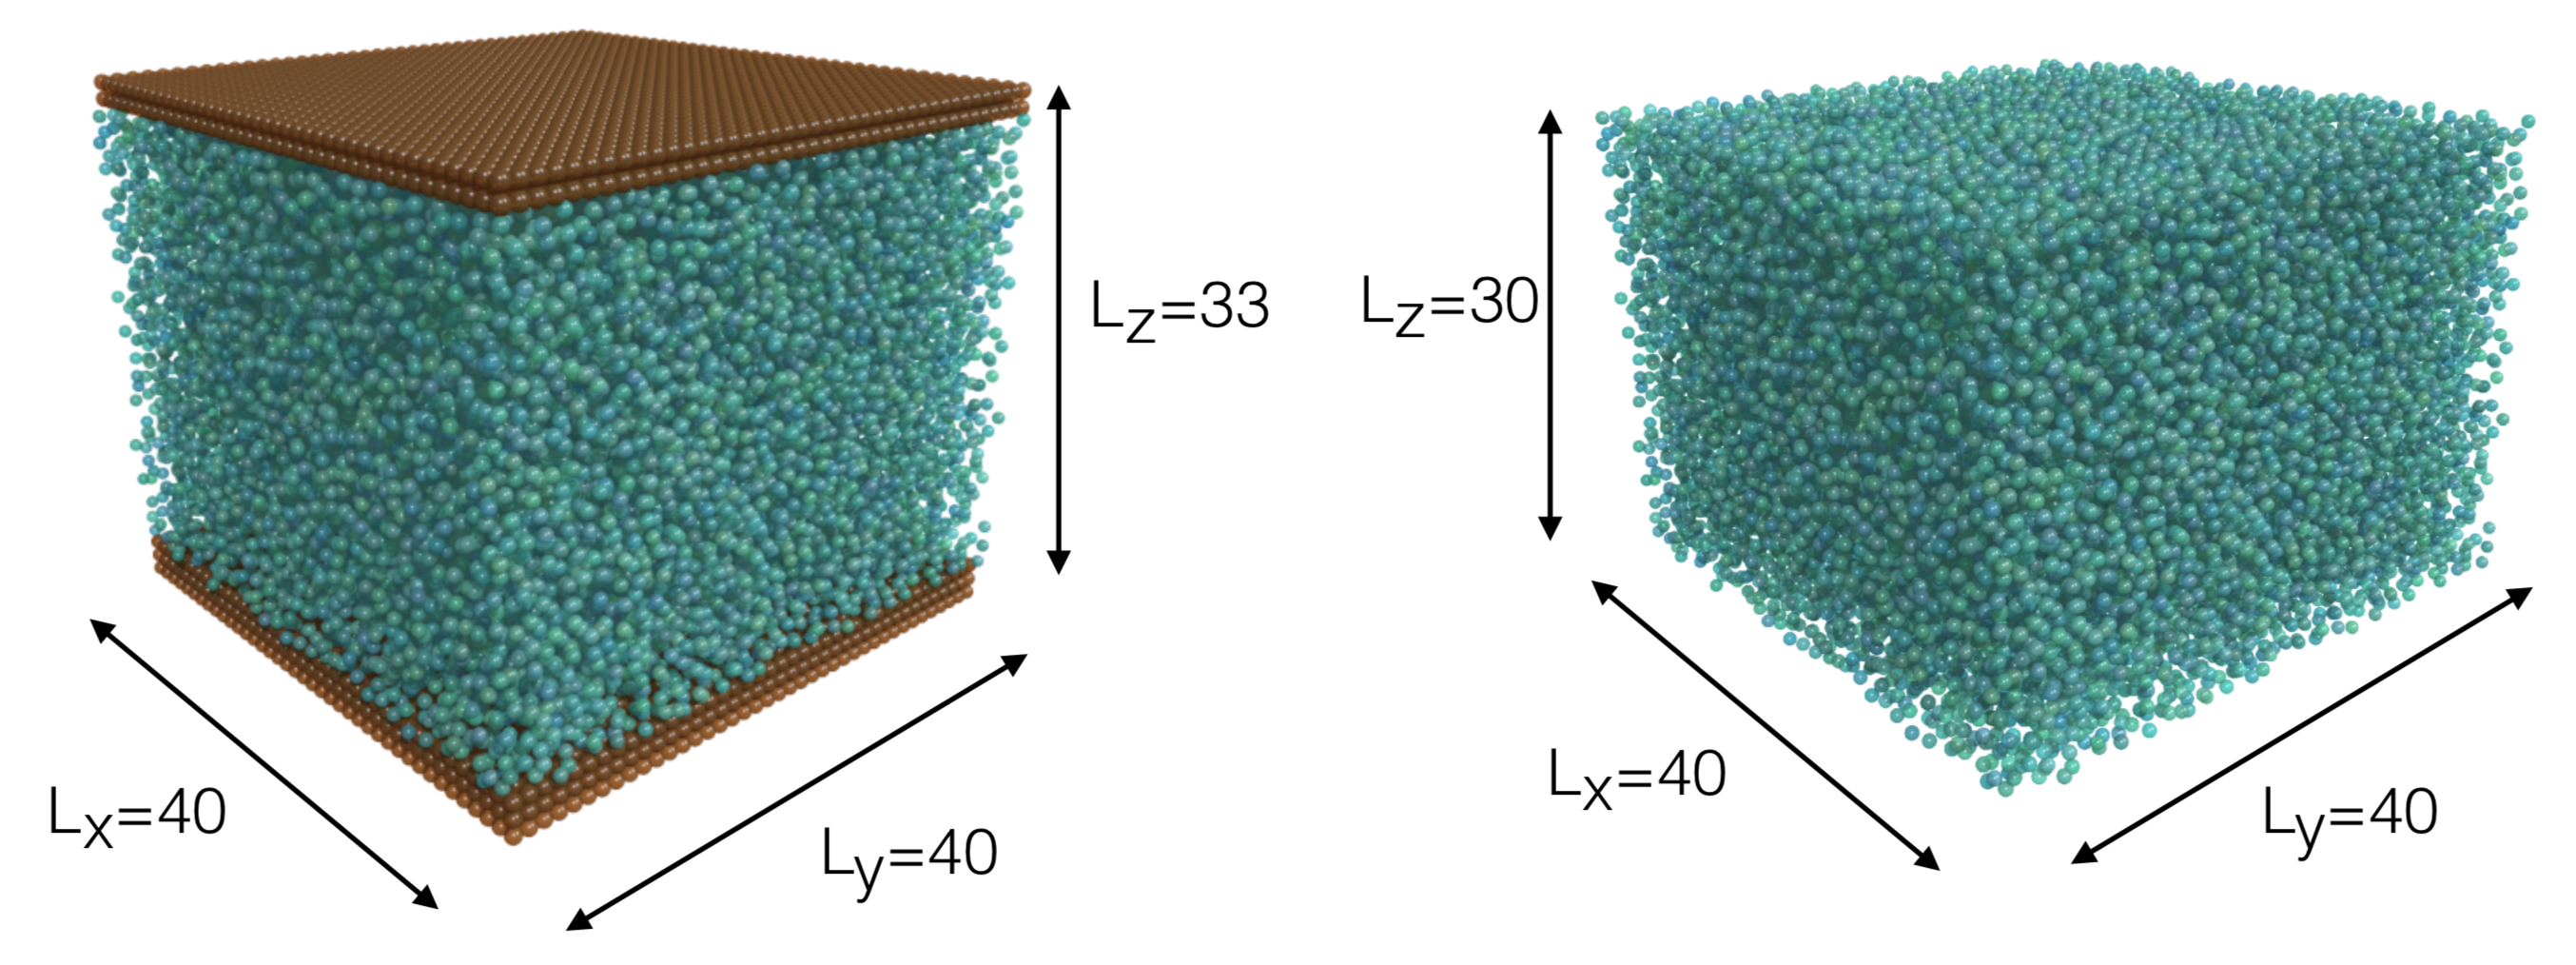
\includegraphics[width=0.8\linewidth]{dim-sim-pbc-walls}
\end{figure}
    \begin{itemize}
      \item $L_x=40\sigma$, $L_x=40\sigma$, $L_z=33\sigma$.
     \item $28175$ partículas de fluido. 
     \item Potencial LJ truncado en $2.5\sigma$.
     %\item $dt=2\cdot 10^{-3}$.
    \end{itemize}
\end{frame}

\begin{frame}{Simulaciones fluido confinado}
  %\begin{figure}
  %  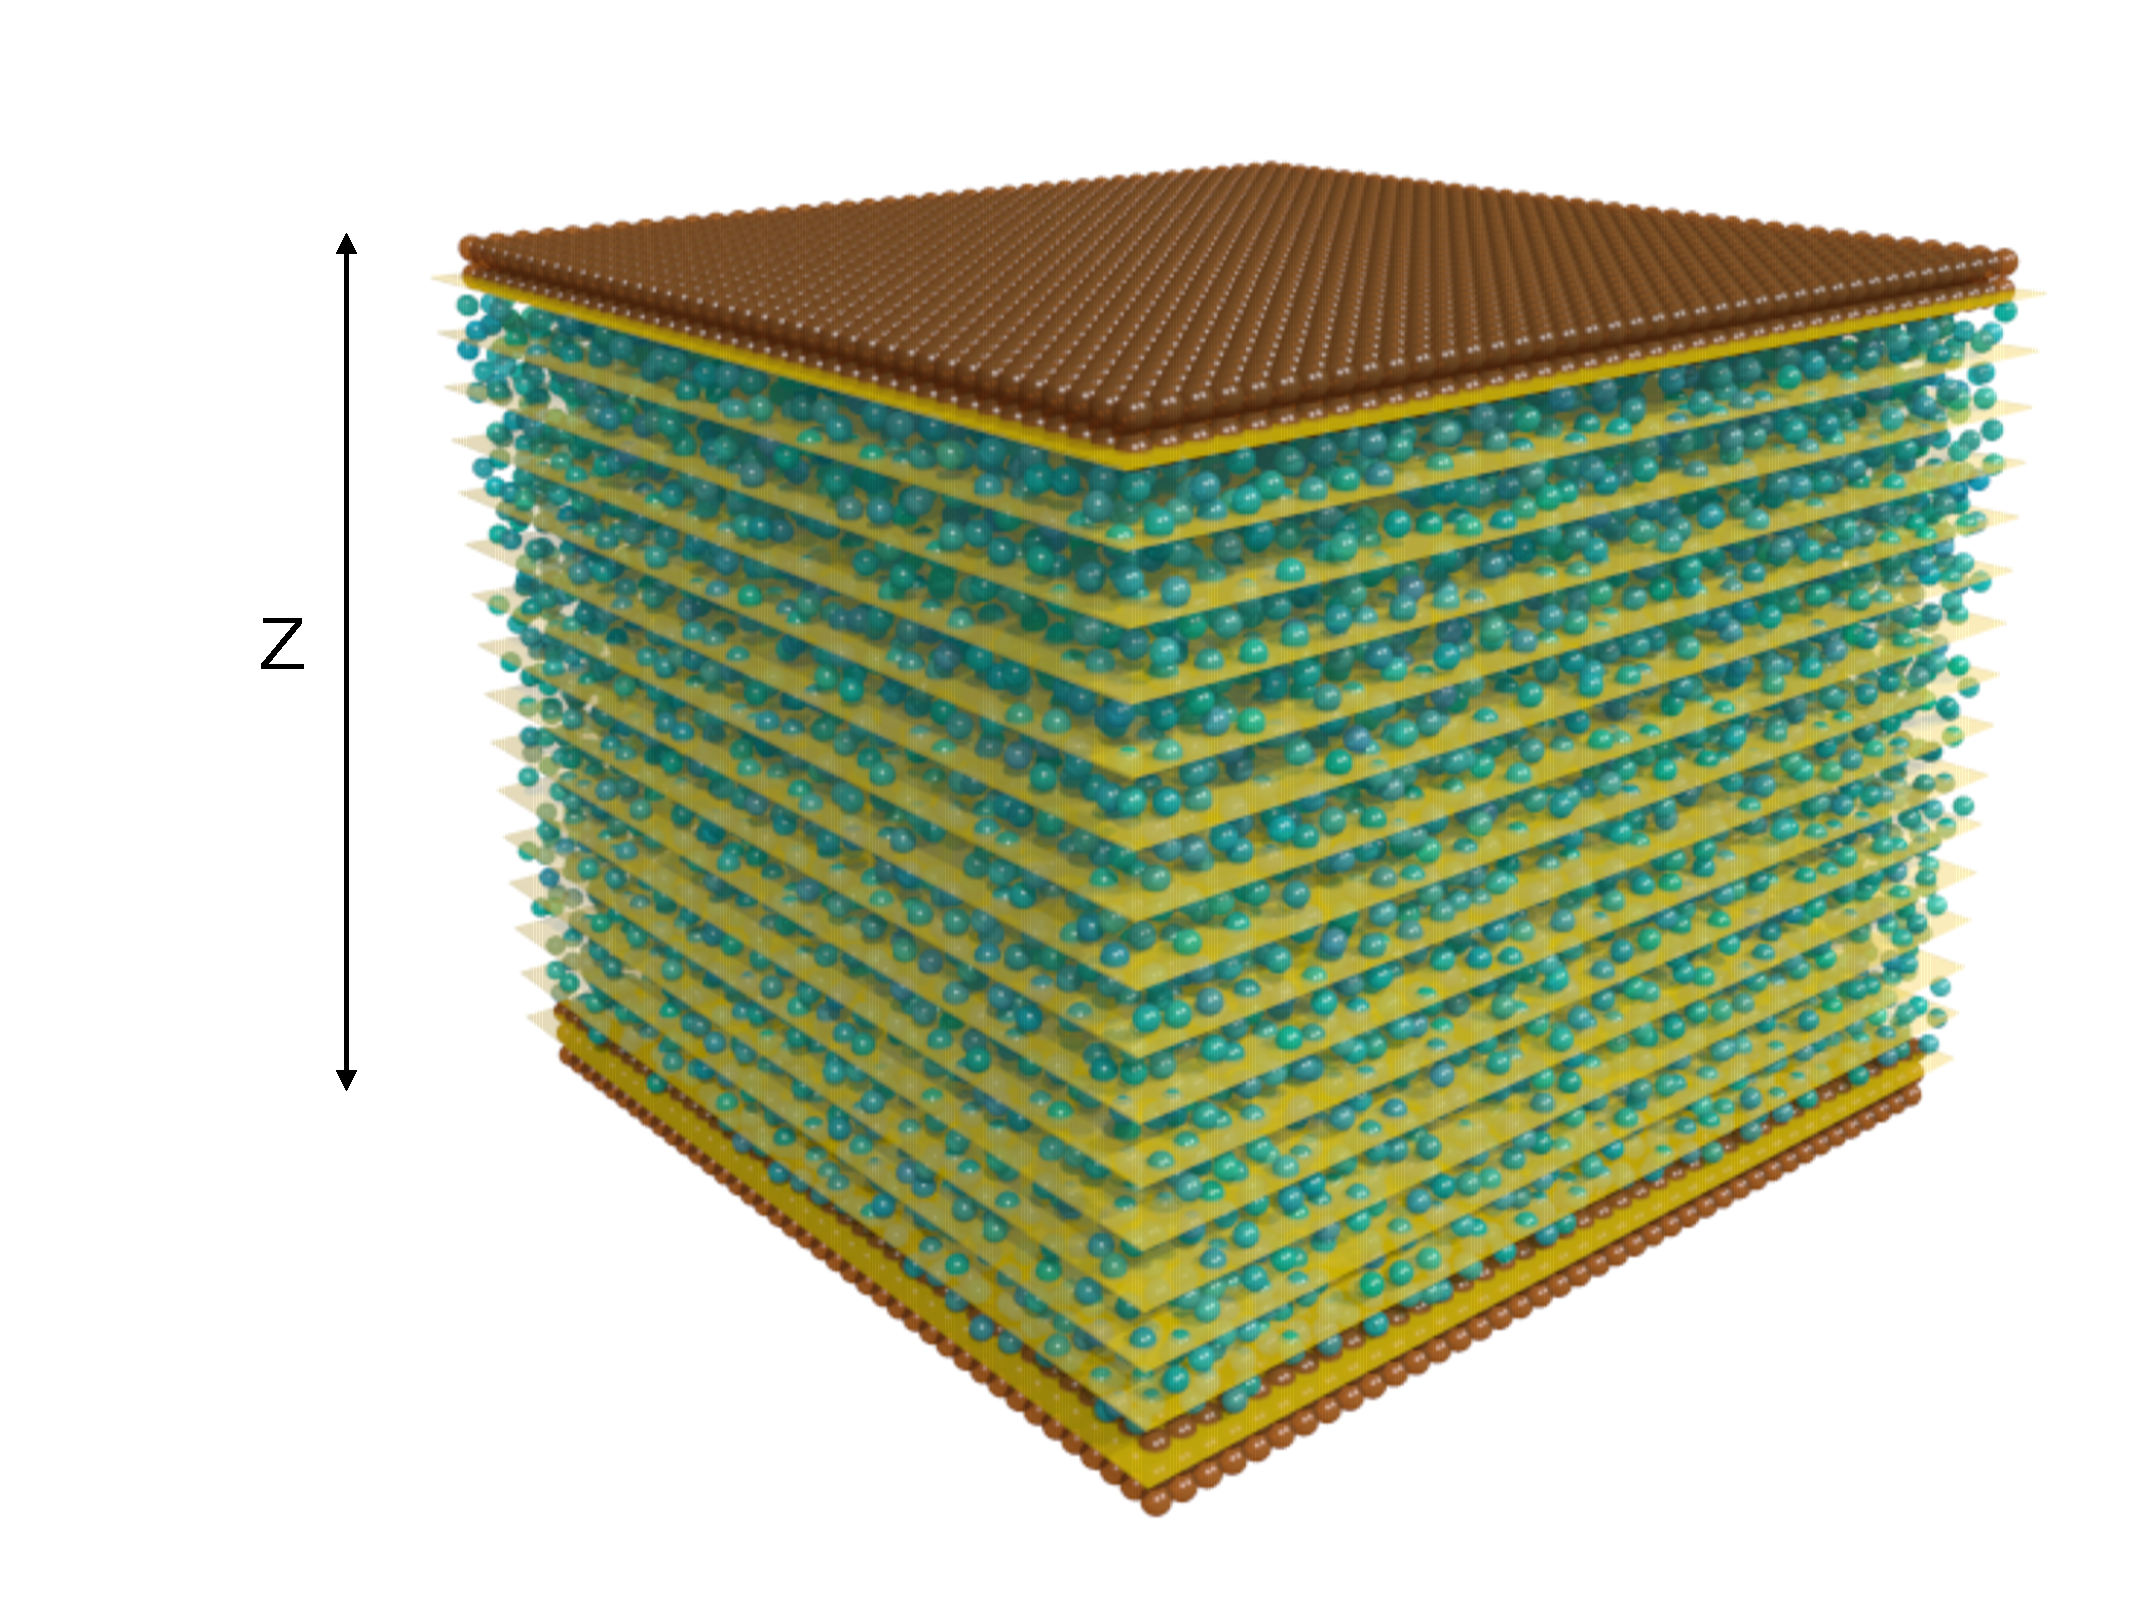
\includegraphics[width=0.5\linewidth]{sim-walls-box-bin}
  %\end{figure}
   \begin{itemize}
     %\item Simulation of $28749$ particles interacting with a LJ potential truncated at $\sigma=2.5$.
     %\item Box size $40x40x30$.
     \item Fase de \alert{equilibrado}
       \begin{itemize}
         %\item Termostato durante $10^5$ pasos de tiempo: $T=2.0$, $\rho=0.6$.
         \item Termostato de Langevin : $T=2.0$, $\rho=0.6$.
         \item Quitamos termostato y dejamos que corra en NVE.
          \end{itemize}
        \item Fase de \alert{producción}
       \begin{itemize}
         %\item $12\times10^6$ pasos de tiempo.
         \item Medición de $g_{\mu}^x(t)$.
           %medido cada $2$ pasos de tiempo.
         \item Eje $z$ discretizado en $66$ bines $\mu$ $\rightarrow$ {$\boldsymbol{\Delta} {\bf z=0.5}\boldsymbol{\sigma}$}.
         \end{itemize}
       \item[]
         \begin{figure}
    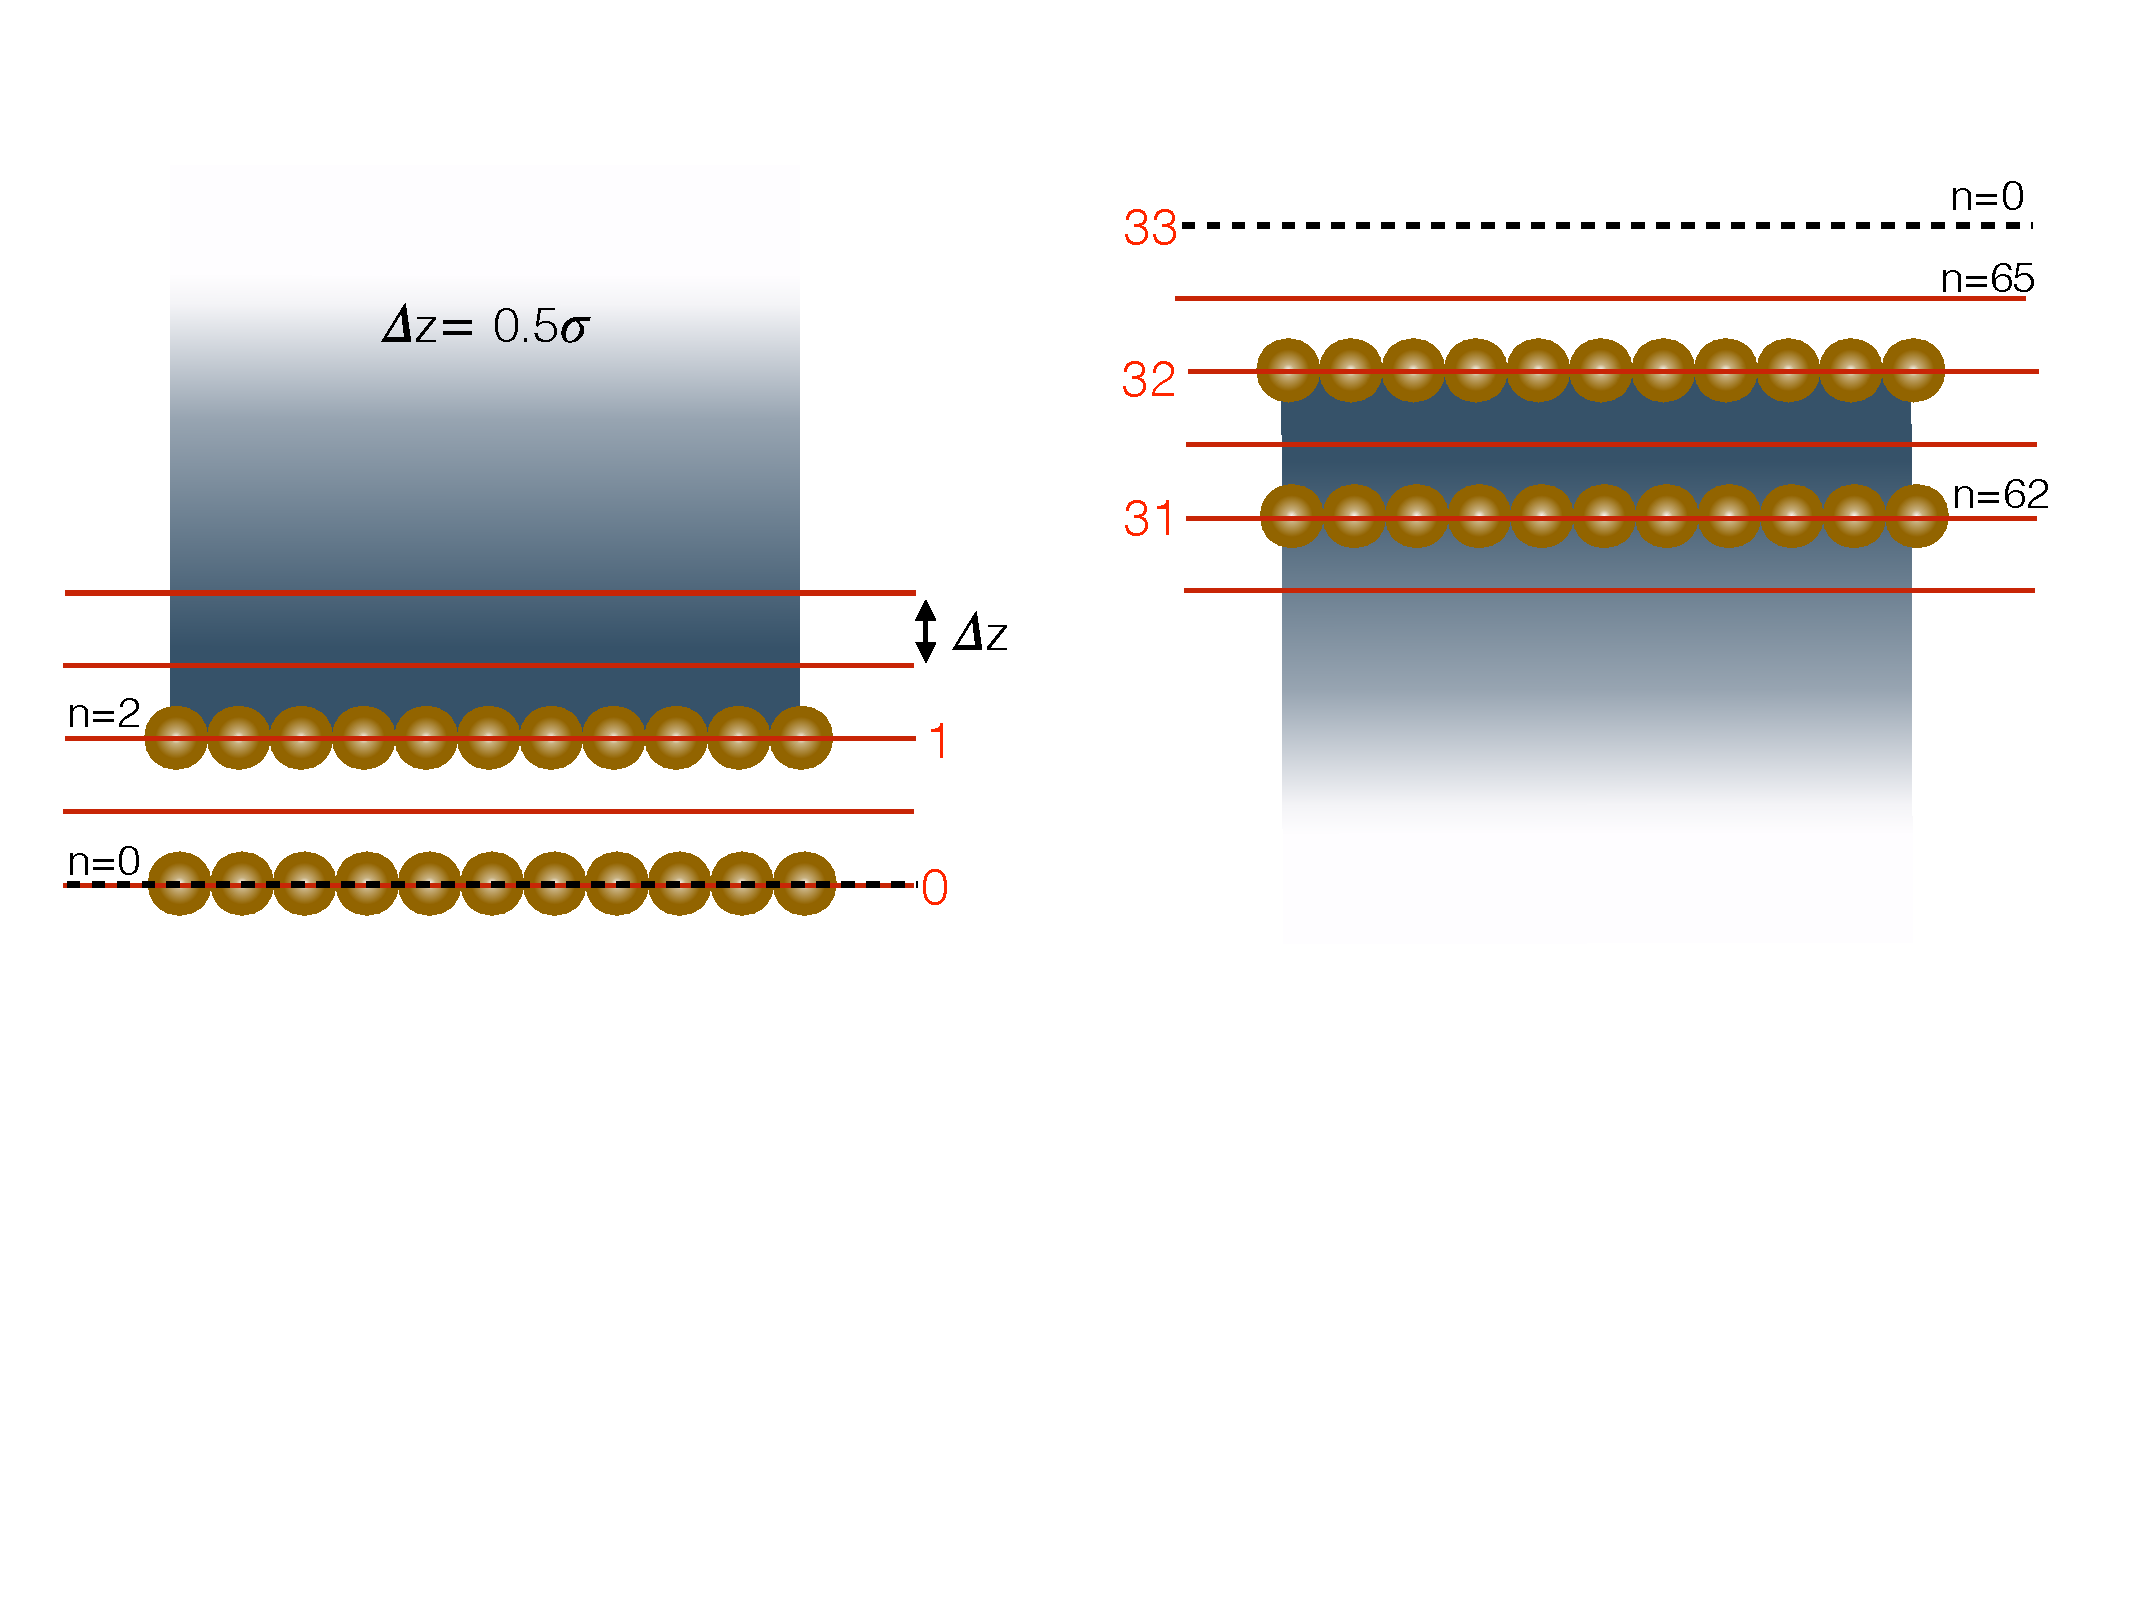
\includegraphics[width=\linewidth]{bin_size_top-bottom}
  \end{figure}
     \end{itemize}

 \end{frame}

%\begin{frame}{The sistema y the CG variables}
%\begin{itemize}
%  \item The sistema
%\begin{figure}
%    \centering
%    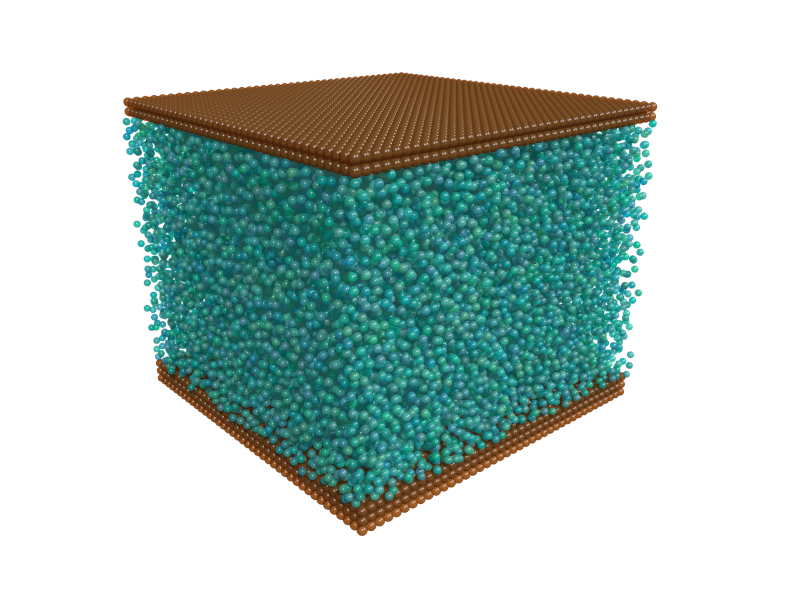
\includegraphics[width=0.45\linewidth]{PRL3_gold2_wo_layers_wo_diffuse}
%    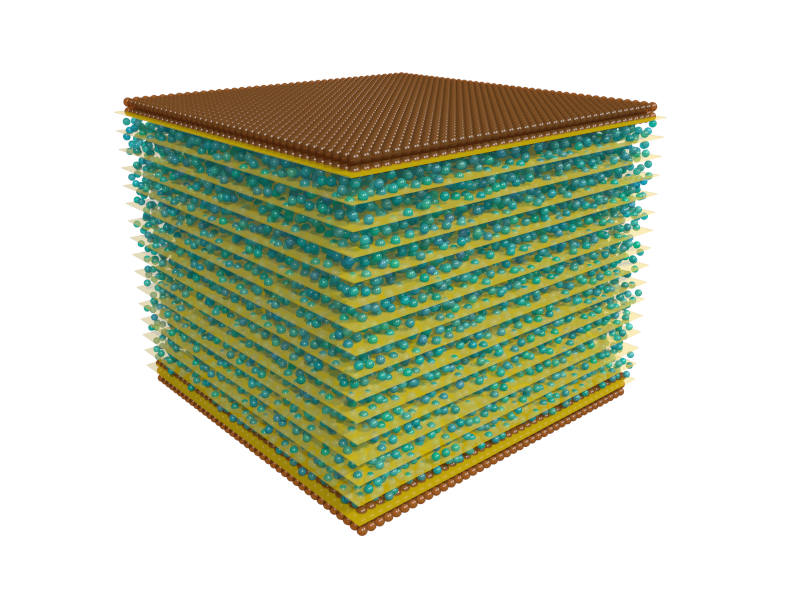
\includegraphics[width=0.45\linewidth]{PRL3_gold2_wo_diffuse}
%\end{figure}
%\item The CG variables y its correlación
%\begin{align}
%  \hat{\bf g}^x_\mu= \sum_i^N{\bf p}_i\delta_\mu({\bf q}_i), && 
%  \hat{g}^T=(\hat{\bf   g}^x_1,\cdots,\hat{\bf  g}^x_{N_{\rm   bin}}), &&
%  C(t)=\llangle \hat{g}(t) \hat{g}^T\rrangle 
%\nonumber
%\end{align}
%\end{itemize}
%\end{frame}
%
%\begin{frame}{Simulation set up}
%   \begin{itemize}
%     \item Simulation of $28175$ fluid particles interacting with a LJ potential truncated at $\sigma=2.5$.
%     \item Two solid walls in the $xy$ plane confine the fluid.  
%     \item Box size $40x40x33$. 
%     \item $dt=0.002$ in reduced units.
%     \item Equilibration stage
%       \begin{itemize}
%         \item Langevin thermostat for $10^5$ timesteps: $T=2.0$, $\rho=0.6$.
%         \item NVE microcanonical conditions for a further $10^5$ timesteps.
%          \end{itemize}
%        \item Production stage
%       \begin{itemize}
%         \item $12\times10^6$ timesteps.
%         \item $z$ axis binned in $66$ bins $\mu$ $\boldsymbol{\Delta} {\bf z=0.5}\boldsymbol{\sigma}$ or $33$ bins $\mu$ $\boldsymbol{\Delta} {\bf z=2} \boldsymbol{\sigma}$.
%         \item $g_{\mu}^x(t)$ recorded every $2$ timesteps. 
%         \end{itemize}
%     \end{itemize}
%\end{frame}
%
%\begin{frame}{Reciprocal space}
%  \begin{itemize}
%    \item Eigenvalues $\tilde{C}_{\mu}$ y eigenvectors $u_{\mu}$
%\begin{align}
%  C(t)&=\sum_\mu^{N_{\rm bin}}\tilde{C}_\mu(t) u_\mu(t) \otimes u_\mu^T(t)
%\nonumber
%\end{align}
%    \item Unitary matrix $E(t)$
%\begin{align}
%  E^{-1}(t)\esc C(t)\esc E(t)=\tilde{C}(t)
%\nonumber
%\end{align}
%\item We observed that $\dot{E}\simeq 0$.
%\item The predictions of $C(t)$ in the reciprocal space
%\begin{align}
%  \tilde{C}_\mu(t)&=\exp\{-\tilde{\Lambda}_{\mu\mu} (t-\tau)\}  \tilde{C}_\mu(\tau)
%  \nonumber
%\end{align}
%    \end{itemize}
%\end{frame}

\begin{frame}{Bines finos ($\Delta z=0.5\sigma$)}
  \begin{itemize}
    \item<1-> $C_{\mu\nu}(t)$ en  $t=0$ (izq.) y $t=0.6$ (dcha.).
\begin{figure}[h!]
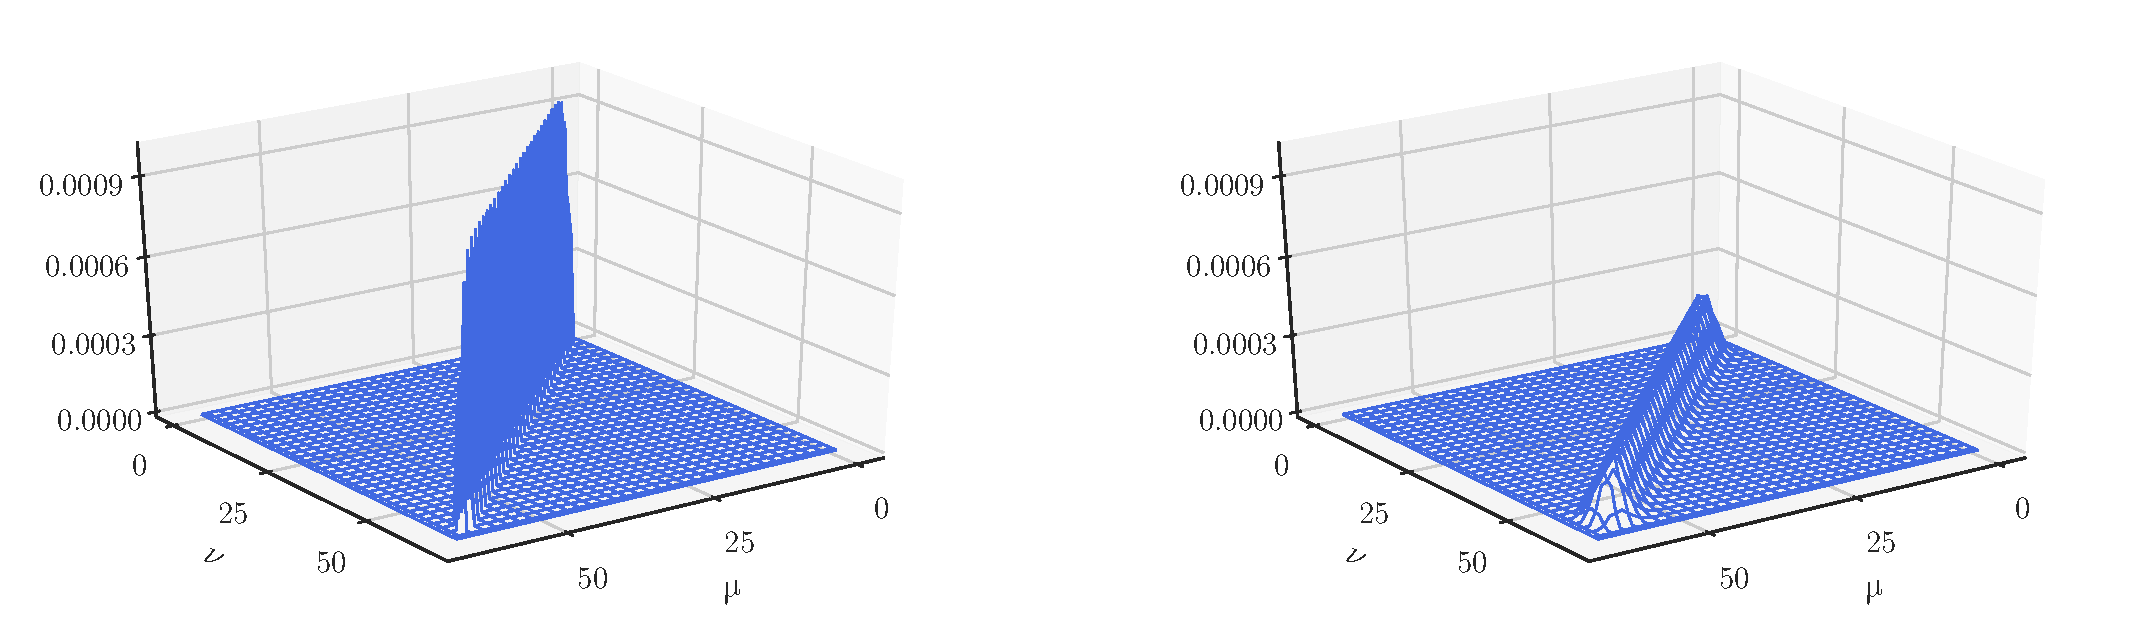
\includegraphics[width=\linewidth]{Ct-matrix-WALLS-66nodes}
\end{figure}
\item<2-> Evolución de los autovalores $\tilde{C}_{\mu\nu}(t)$
\begin{figure}[h!]
  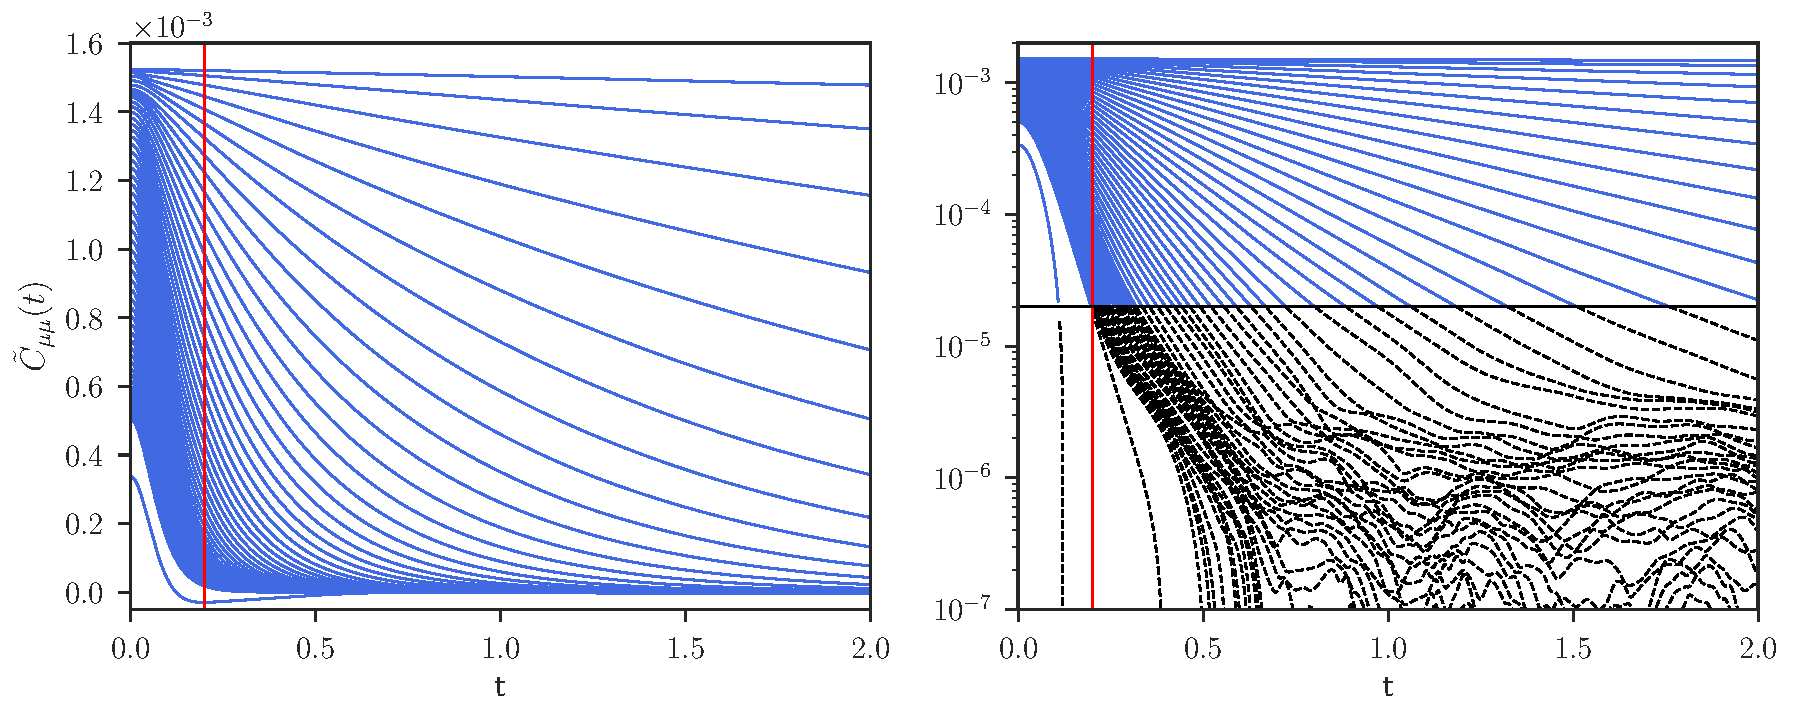
\includegraphics[width=\linewidth]{CtRec-WALLS-66nodes-exp}
\end{figure}
\end{itemize}
\end{frame}

\begin{frame}{Autovalores y autovectores cerca de las paredes ($\Delta z=0.5\sigma$)}
%    The eigenvalues $\tilde{C}_{\mu}(t)$ of the correlación matrix $C(t)$ for $\mu=59,60$ which are identical y superimpose (left) y the corresponding eigenvectors $u_{\mu}$ in blue y orange, respectively (right).
  
  Comportamiento \textbf{no Markoviano} cerca de las paredes. 
  \begin{figure}[h!]
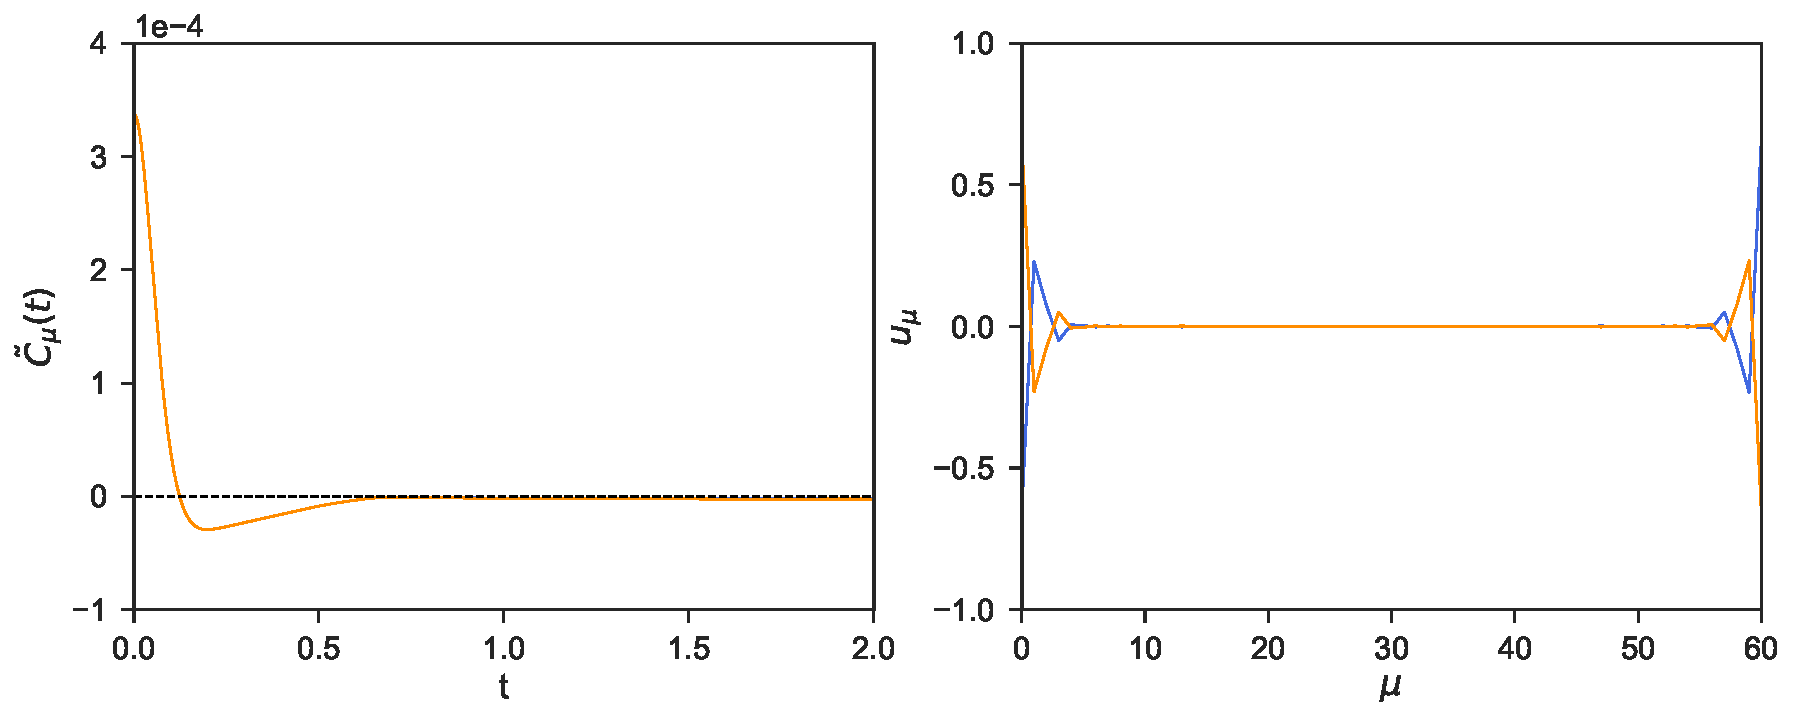
\includegraphics[width=1\linewidth]{EigenvaluesVectors-WALLS-66nodes}
\end{figure}
\end{frame}
%Los autovalores $\tilde{C}_{\mu}(t)$ de $C(t)$ para $\mu={\color{blue}59},{\color{orange}60}$ y sus correspondientes autovectores $u_{\mu}$ .

\begin{frame}{Elementos de la diagonal, $\tilde{\Lambda}(t)$ ($\Delta z=0.5\sigma$)}
%Elementos de la diagonal,
%  $\tilde{\Lambda}_{\mu\mu}(t)$, de $\Lambda(t)$ en el espacio recíproco. 
  %(longitud de onda larga).
\begin{align}
  \tilde{\Lambda}_{\mu\mu}=-\frac{1}{\tilde{C}_{\mu\mu}(t)}\frac{d\tilde{C}_{\mu\mu}}{dt}(t)
  \nonumber
\end{align}
\begin{figure}[h!]
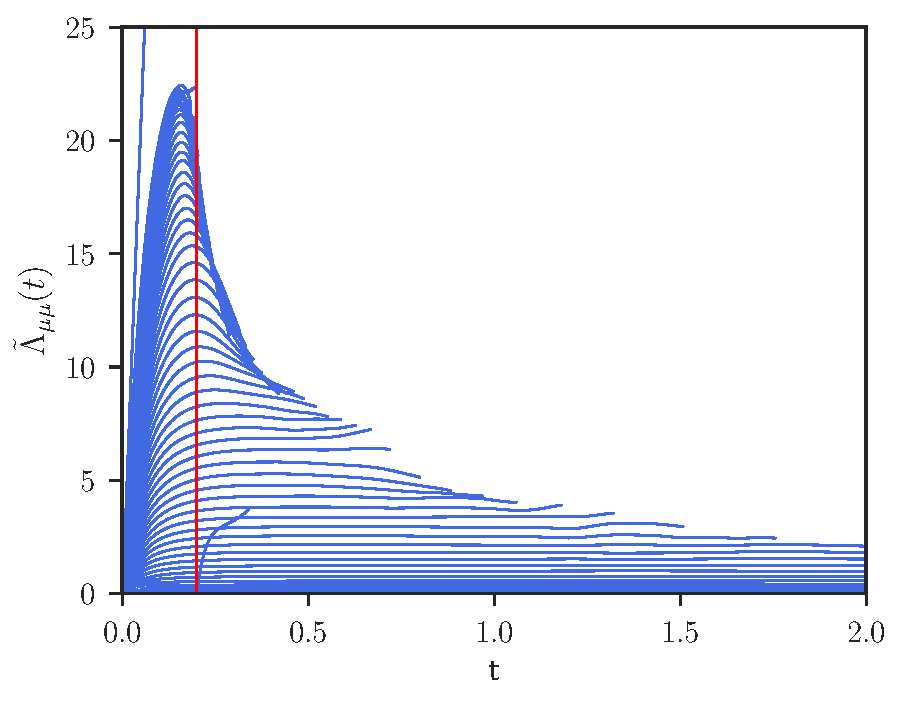
\includegraphics[width=0.7\linewidth]{LambdatRec-WALLS-66nodes}
\end{figure}
  Para $t>0.2$ se observa un \textit{plateau} para los modos inferiores.
\end{frame}

\begin{frame}{Predicciones en el centro del canal ($\Delta z=0.5\sigma$)}
  \begin{align}
    C(t) = {\rm exp}\{-\Lambda^*(t-\tau)\cdot C(\tau)\}
    \nonumber
  \end{align}
La {\color{orange} predicción} en el centro del canal se ajusta perfectamente  a la {\color{blue} medición} para $\tau>0.2$.
  
\begin{figure}[h!]
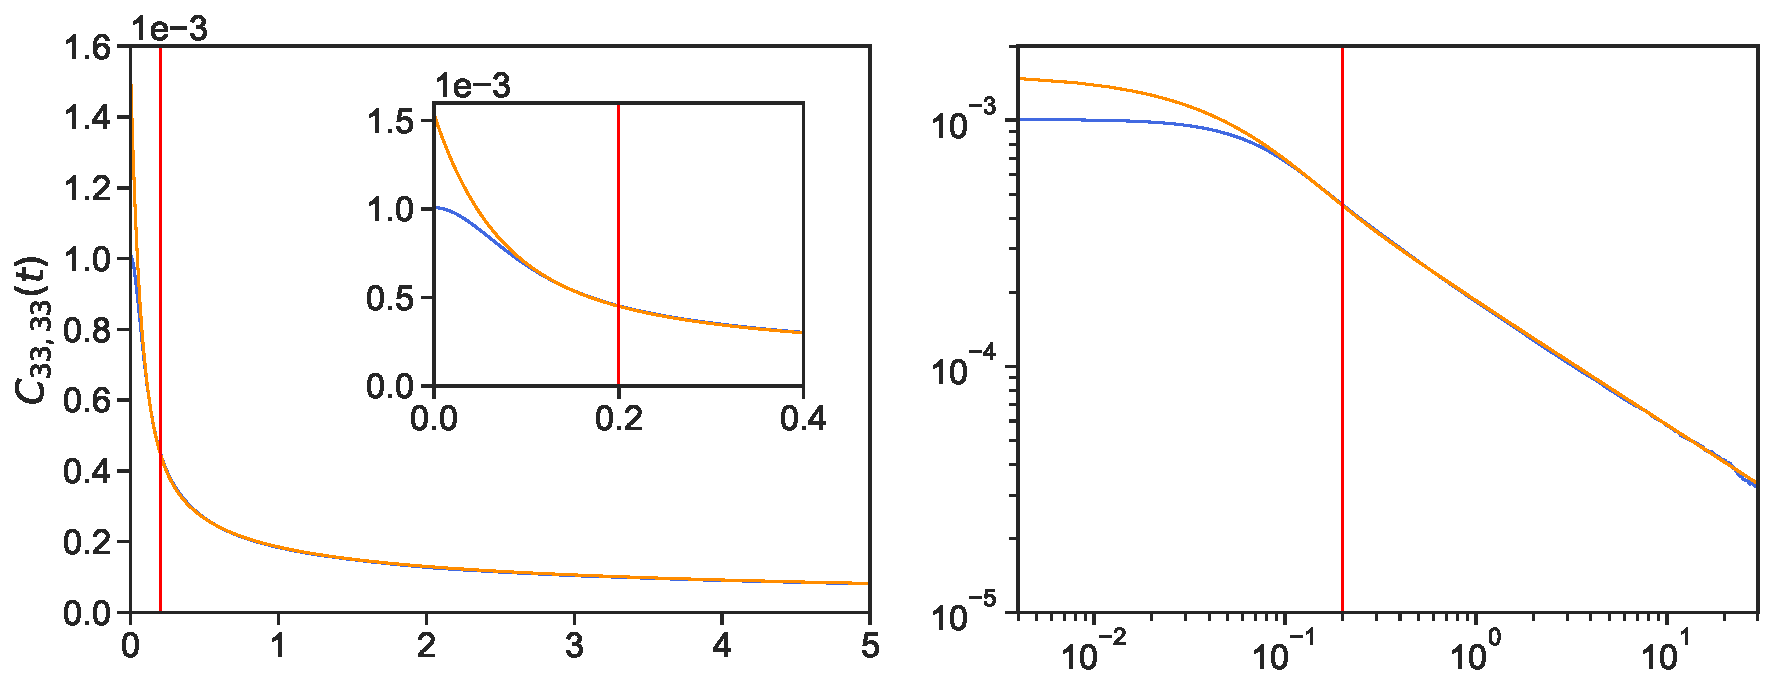
\includegraphics[width=\linewidth]{Predictions-canal-WALLS-66nodes-defense}
\end{figure}
\end{frame}

\begin{frame}{Predicciones cerca de las paredes ($\Delta z=0.5\sigma$)}
\begin{figure}[h!]
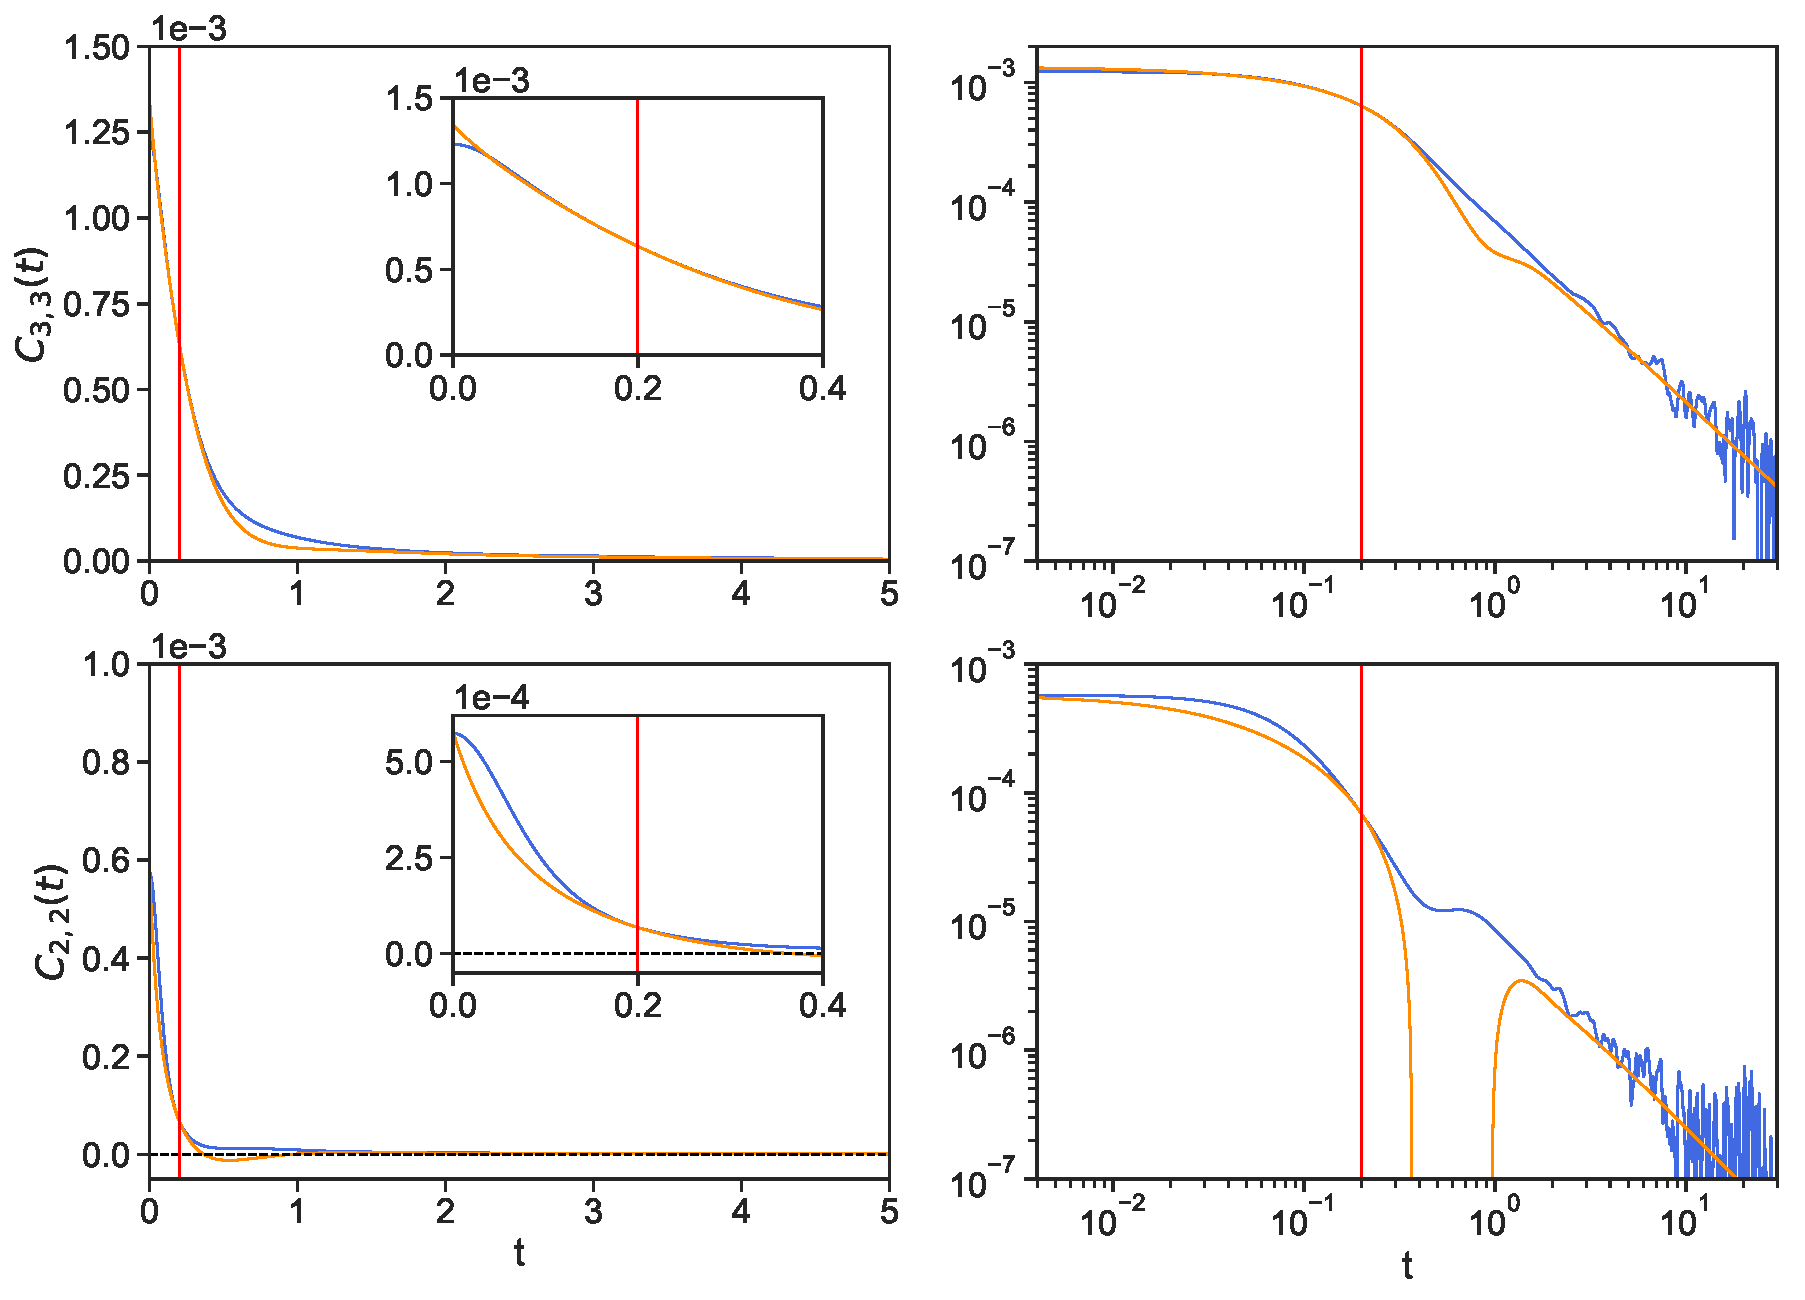
\includegraphics[width=\linewidth]{Predictions-WALLS-66nodes-defense}
\end{figure}
\end{frame}

\begin{frame}{Tamaño de bin: $\Delta z=0.5\sigma$ $\rightarrow$ $\Delta z=2\sigma$}
  %\begin{itemize}
%    \item<1-> We change the size of the bin
%\begin{figure}[h!]
%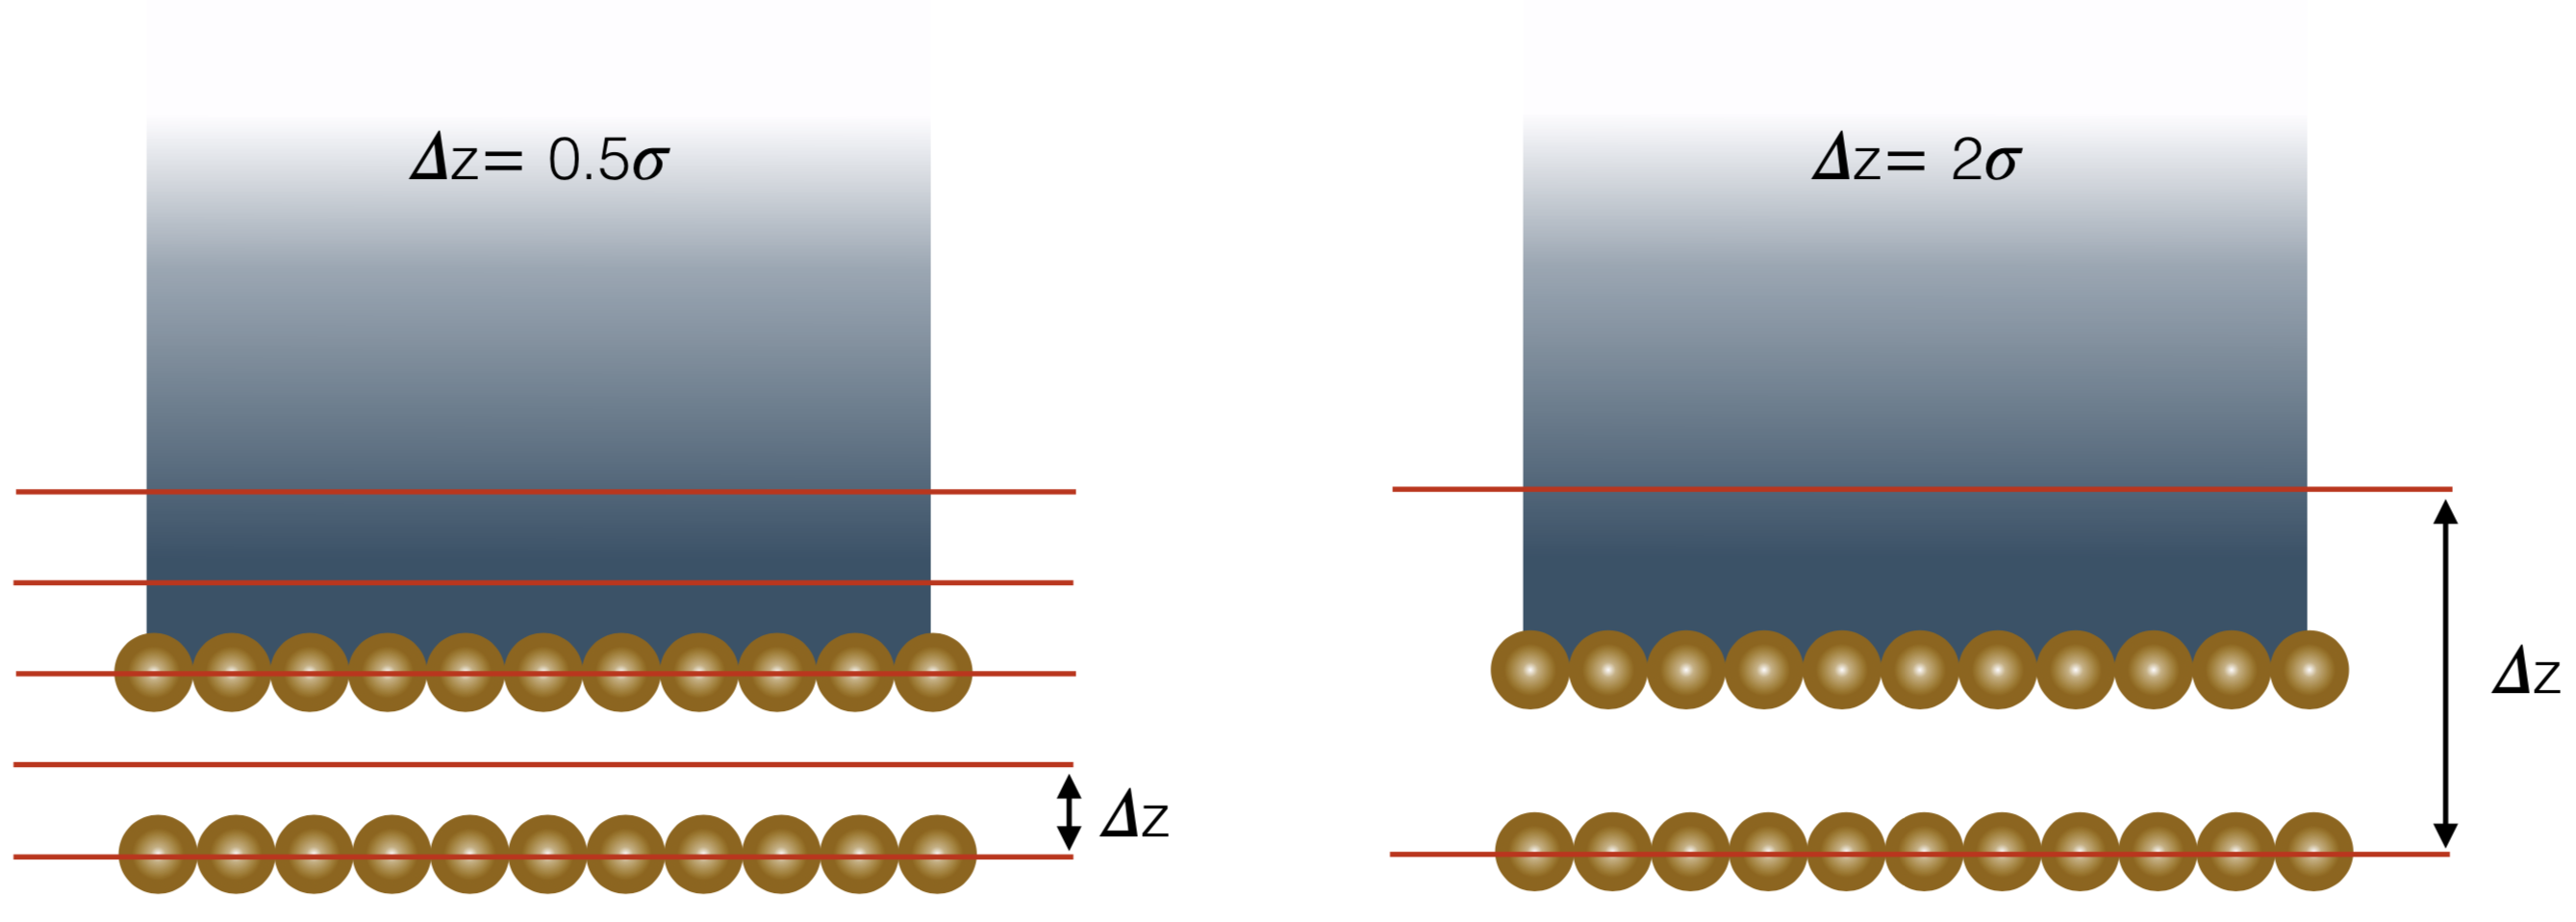
\includegraphics[width=0.7\linewidth]{bin_size}
%\end{figure}
%\item<1-> Bines de tamaño $\Delta z = 2\sigma$: 16 nodos de fluido. 
Bines de tamaño $\Delta z = 2\sigma$ $\rightarrow$ 16 nodos de fluido. 
\begin{figure}[h!]
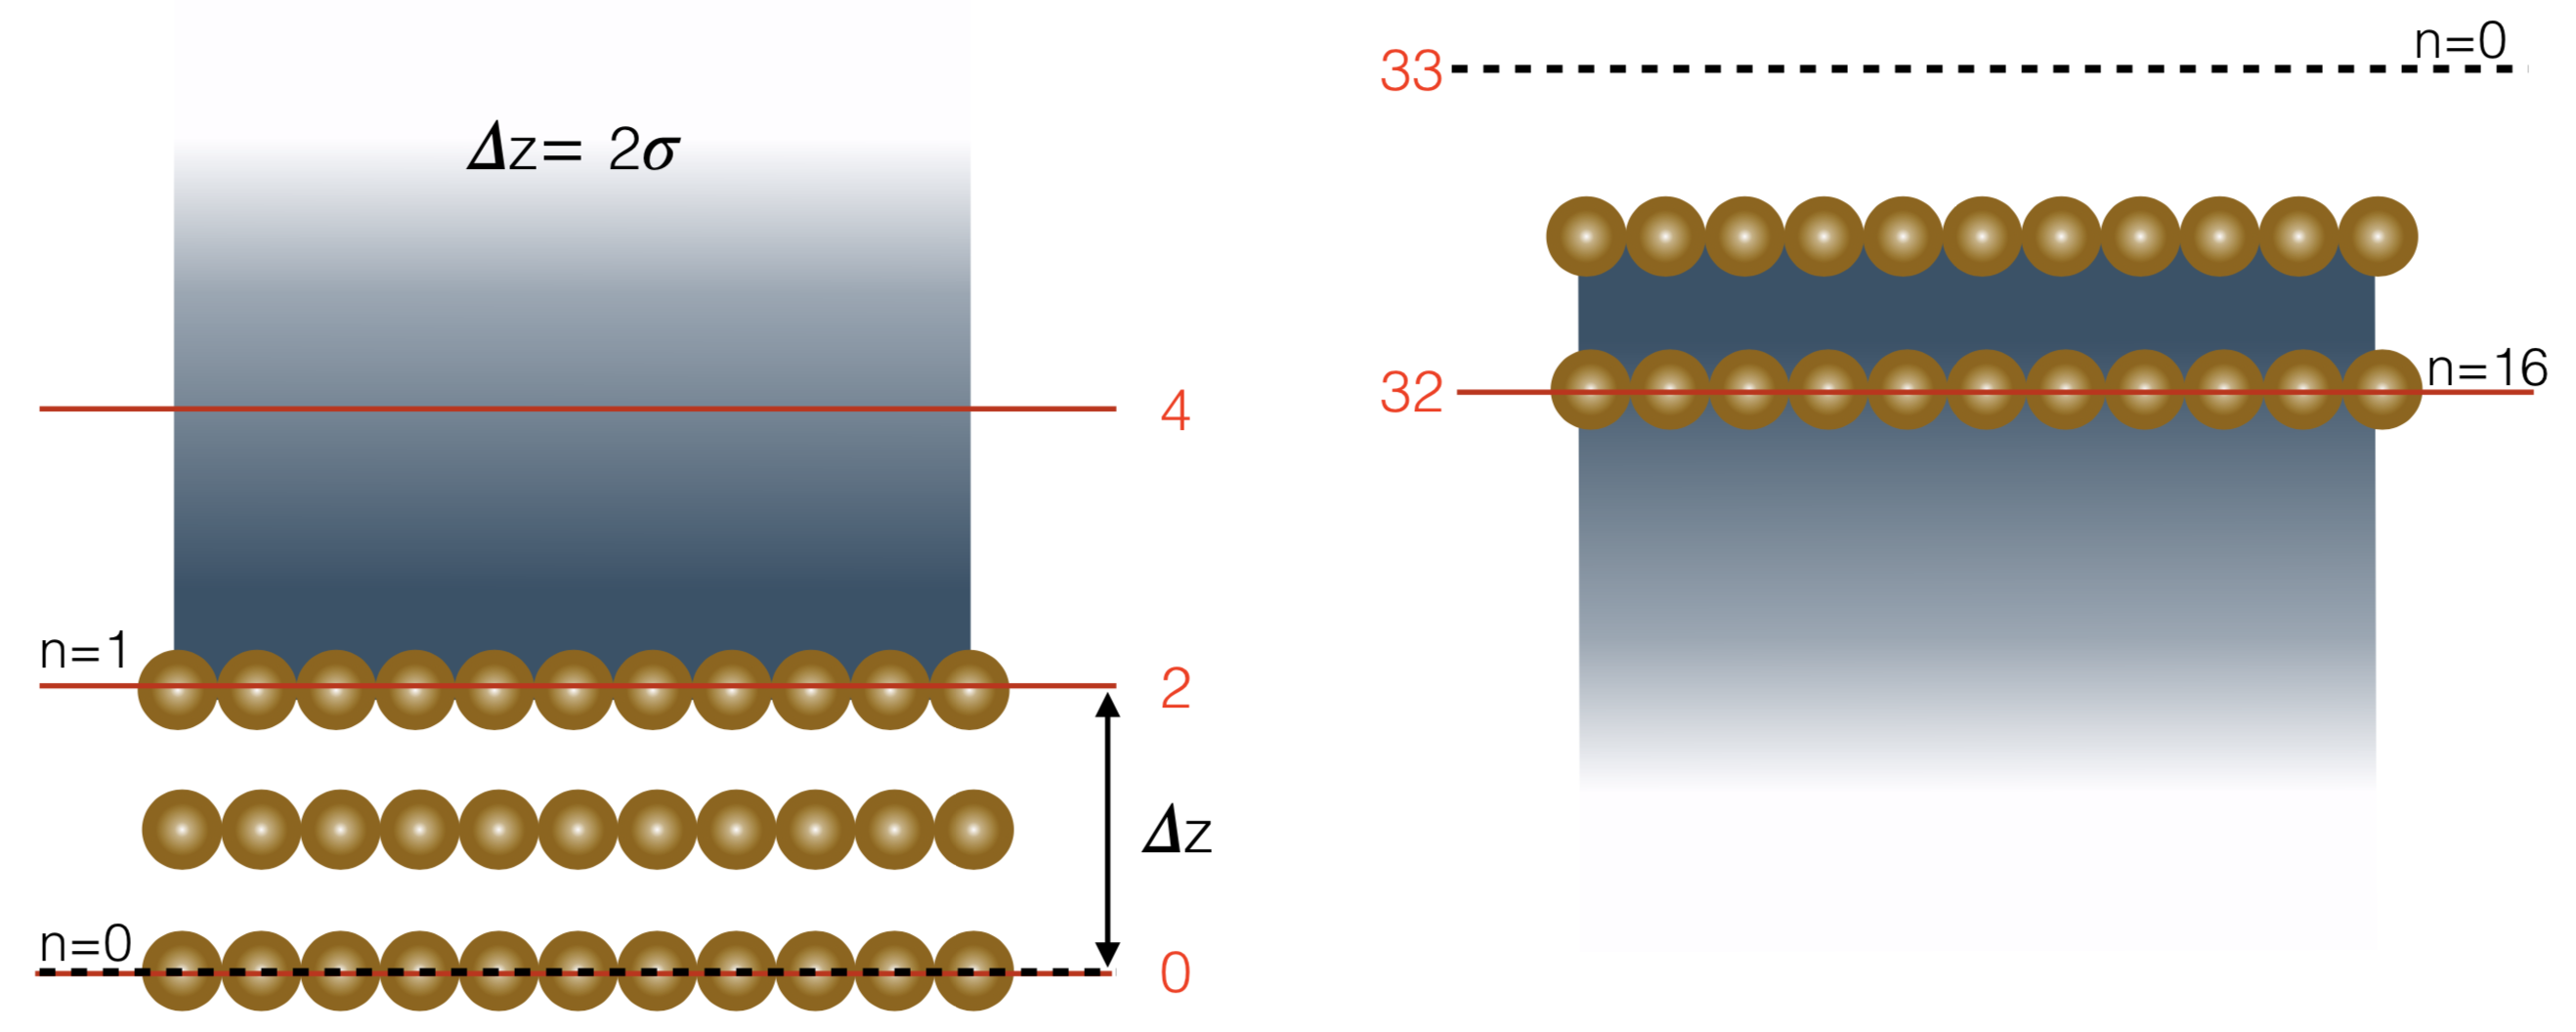
\includegraphics[width=0.75\linewidth]{bin_size-top-bottom_17nodos_cut}
\end{figure}
%\item<2-> Los bines anchos no capturan el \textit{layering} de la densidad.
%\begin{figure}[h!]
%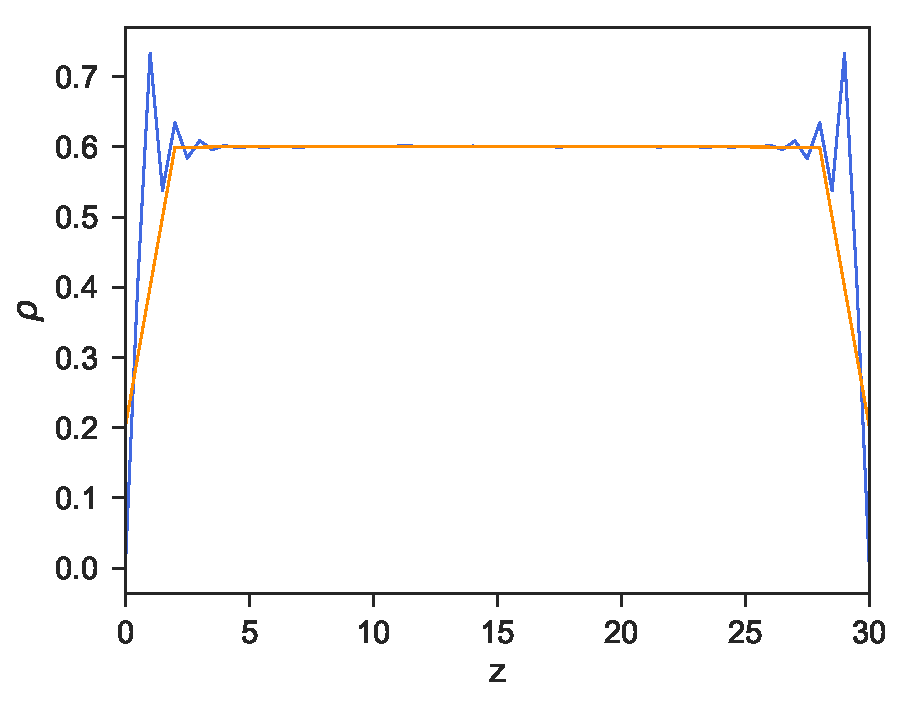
\includegraphics[width=0.48\linewidth]{DensityProfile-WALLS}
%\end{figure}
%  \end{itemize}
\end{frame}

%\begin{frame}{The density layering}
%The thick bins do not capture the layering of the density field.
%\begin{figure}[h!]
%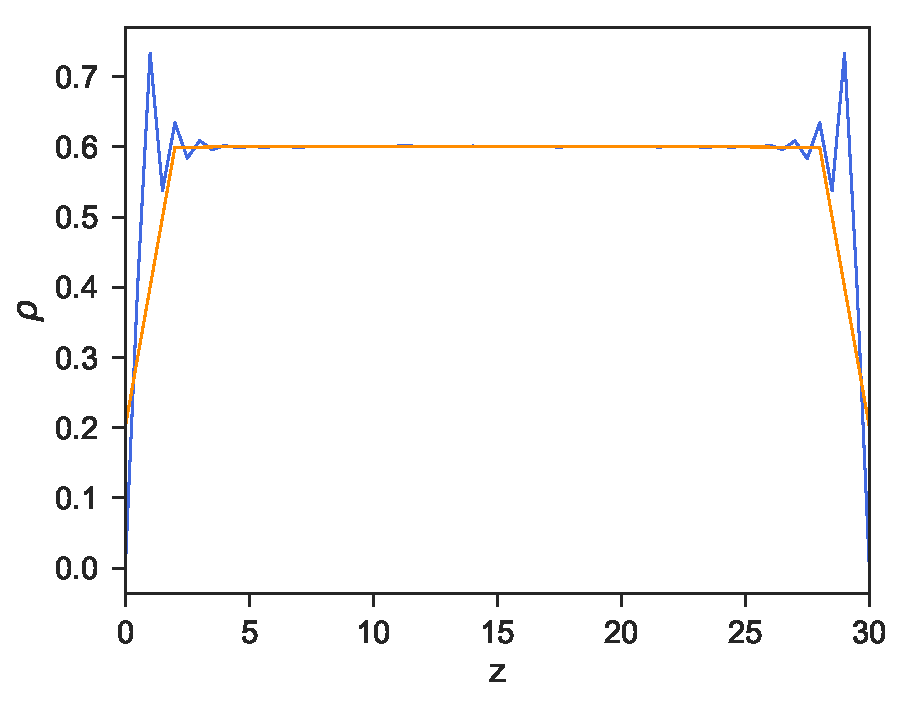
\includegraphics[width=0.7\linewidth]{DensityProfile-WALLS}
%\end{figure}
%\end{frame}


\begin{frame}{Autovalores $\tilde{C}_{\mu\mu}(t)$ ($\Delta z=2\sigma$)}
%Evolution of different eigenvalues $\tilde{C}_{\mu\nu}(t)$. Vertical line  at $t=\tau=0.3$.
  \begin{itemize}
    \item<1->[]
\begin{figure}[h!]
  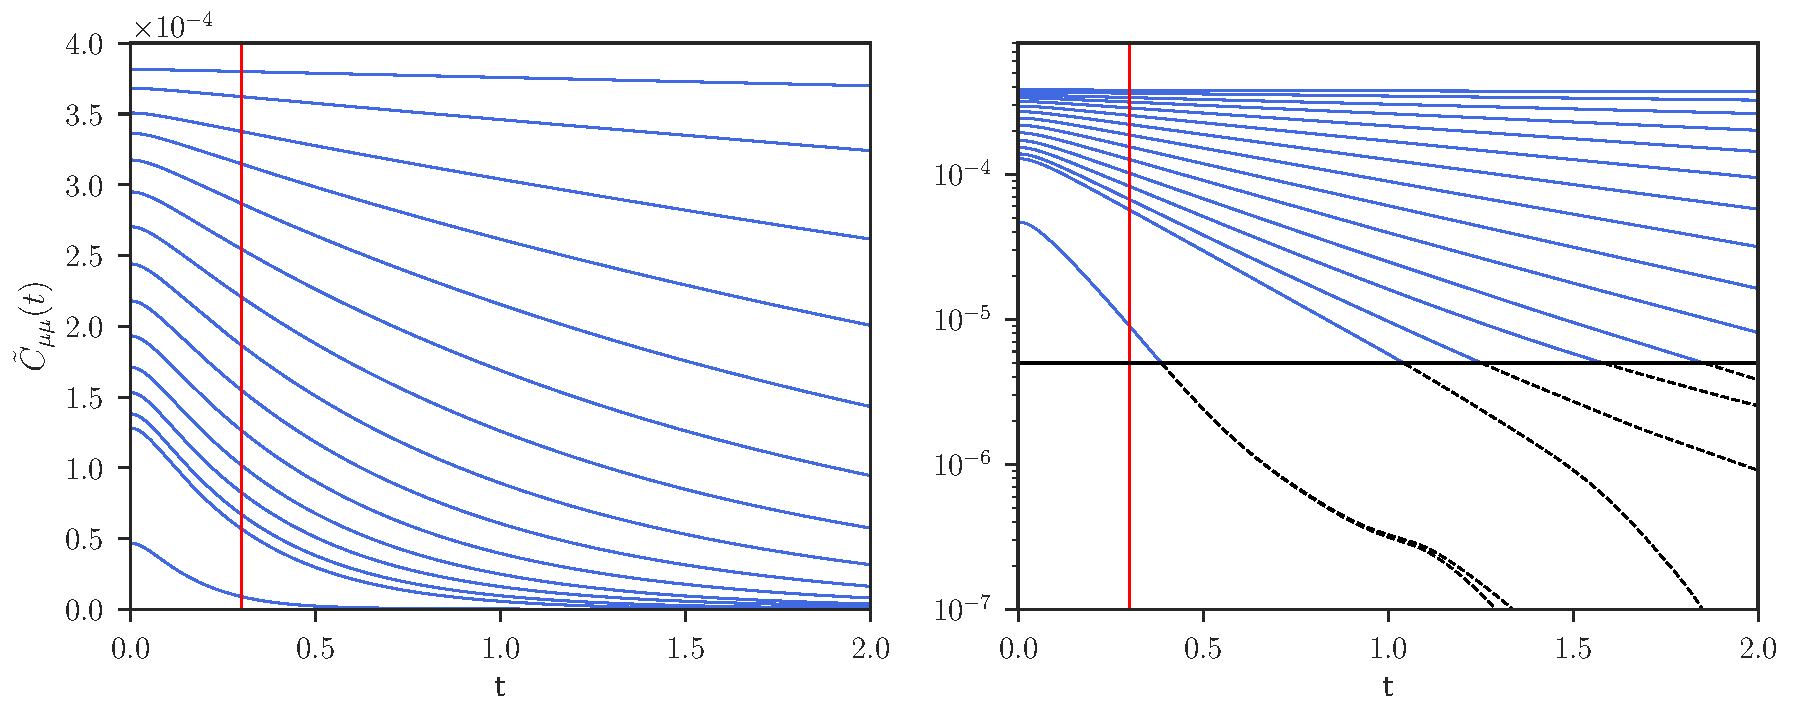
\includegraphics[width=0.97\linewidth]{CtRec-WALLS-17nodes-exp}
\end{figure}
    \item<2->[]
\begin{figure}[h!]
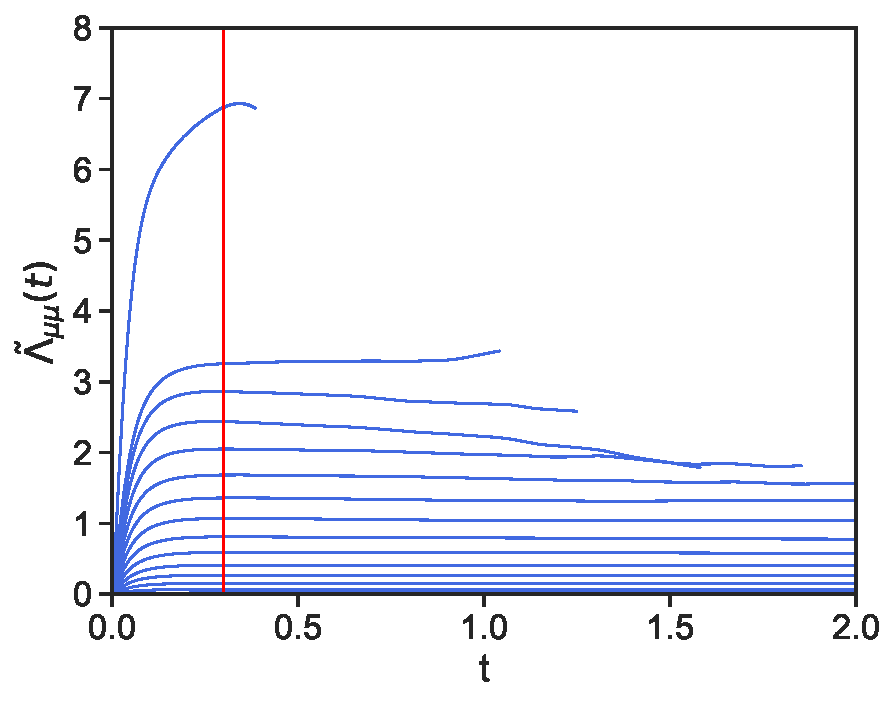
\includegraphics[scale=0.315]{LambdatRec-WALLS-17nodes}
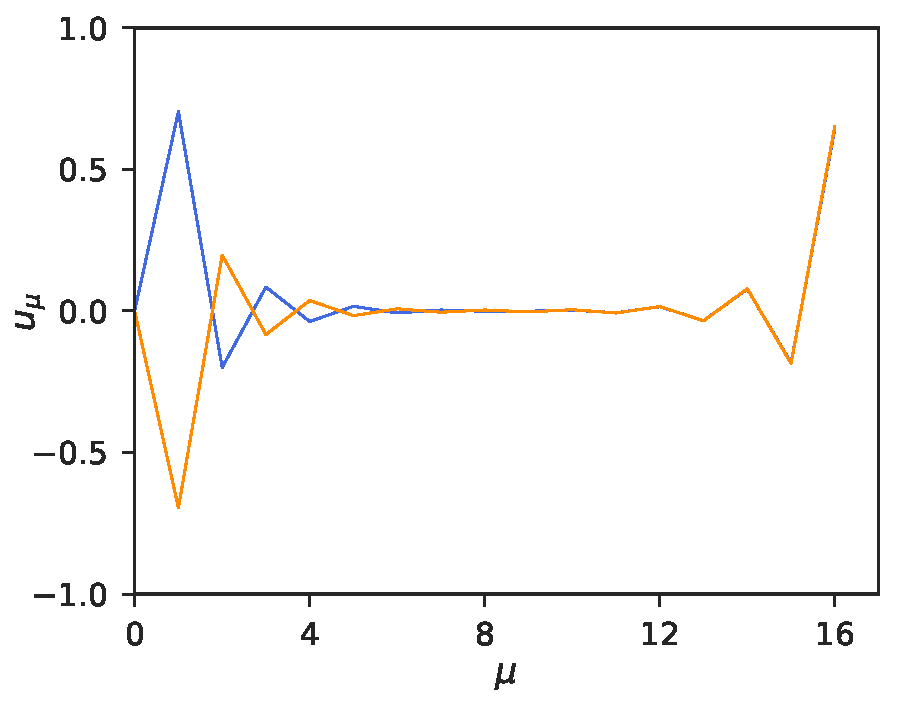
\includegraphics[scale=0.315]{Eigenvectors-WALLS-17nodes}
\end{figure}
  \end{itemize}
\end{frame}

\begin{frame}{Predicción de autocorrelaciones ($\Delta z=2\sigma$)}
\begin{figure}[h!]
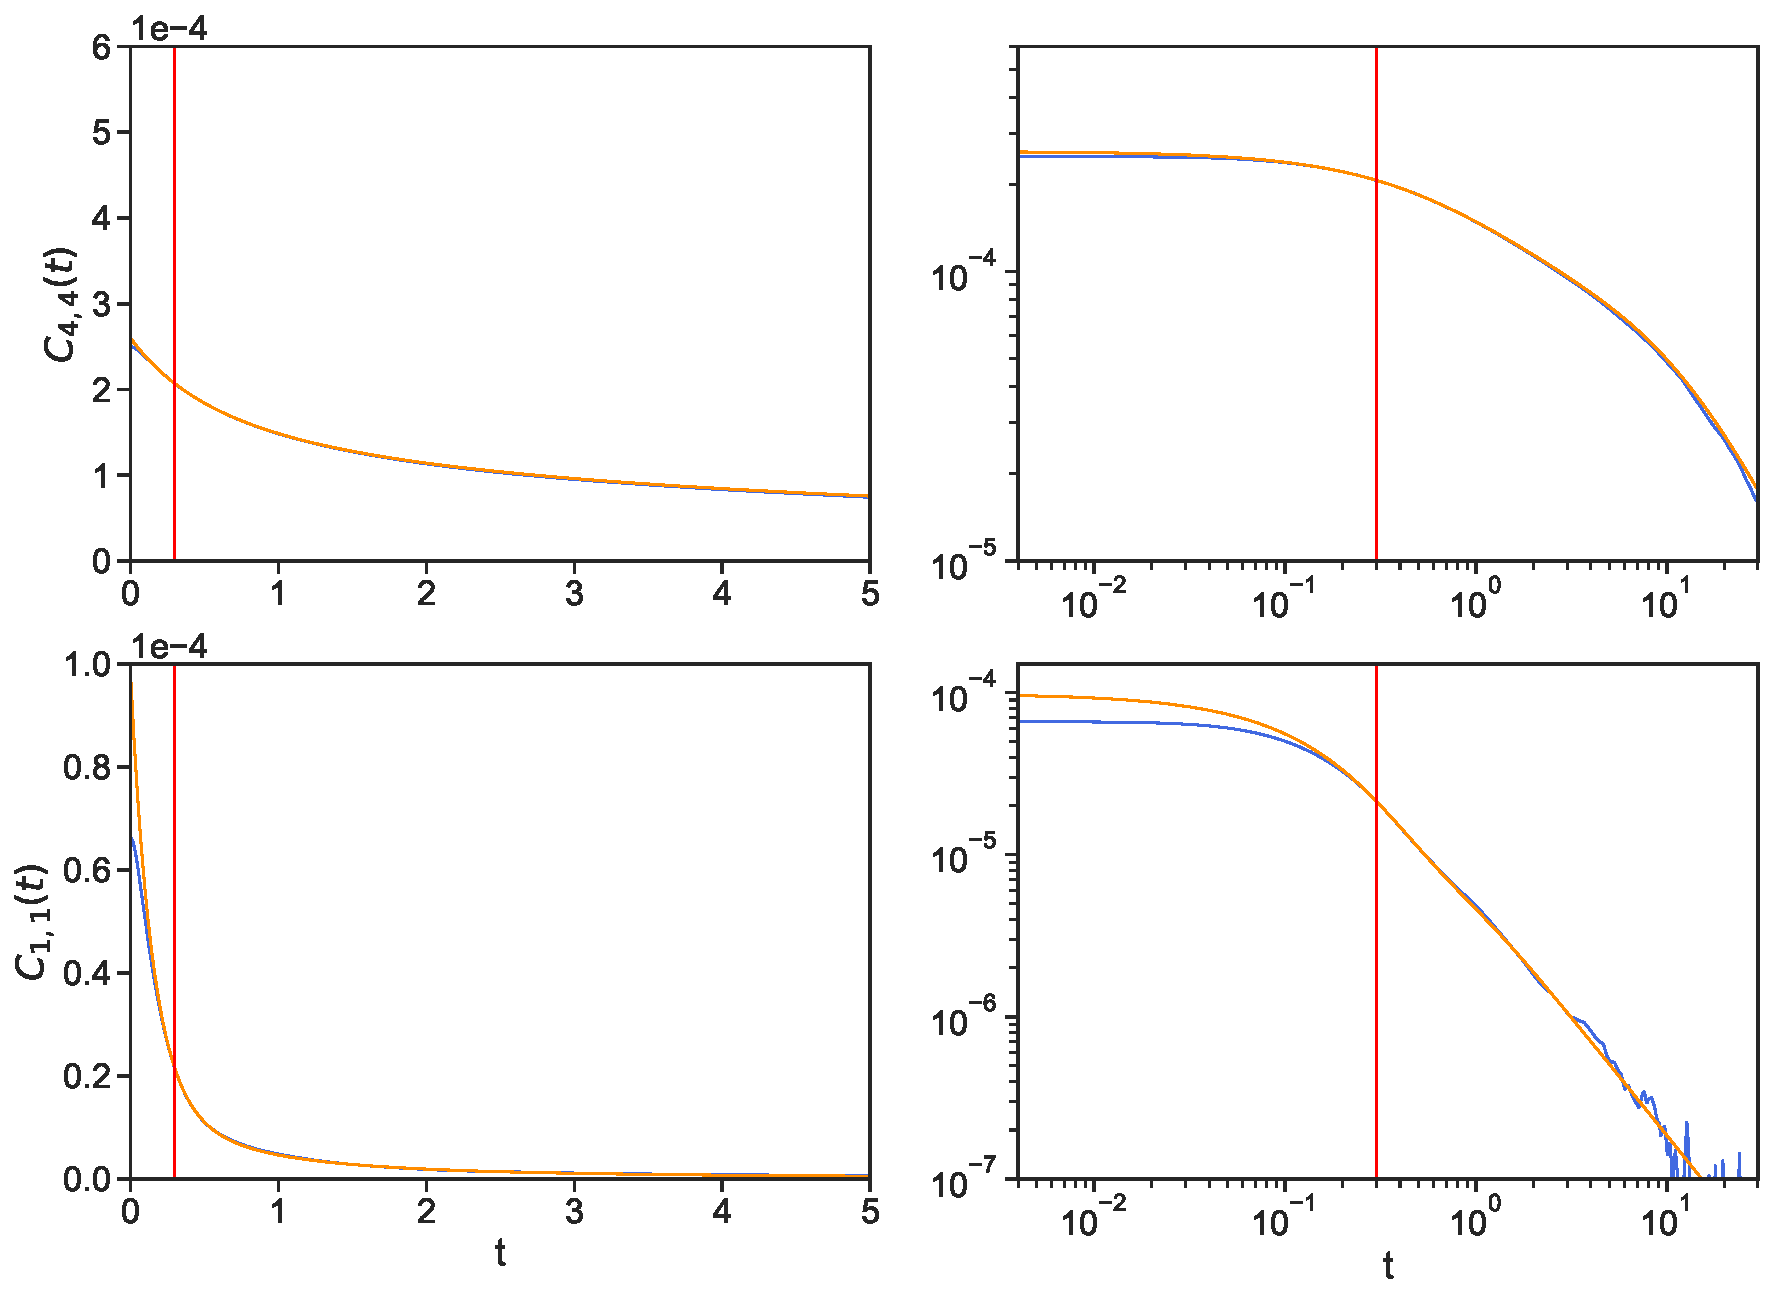
\includegraphics[width=\linewidth]{Predictions-WALLS-17nodes-defense}
\end{figure}
\end{frame}

\begin{frame}{Predicción de correlaciones cruzadas ($\Delta z=2\sigma$)}
\begin{figure}[h!]
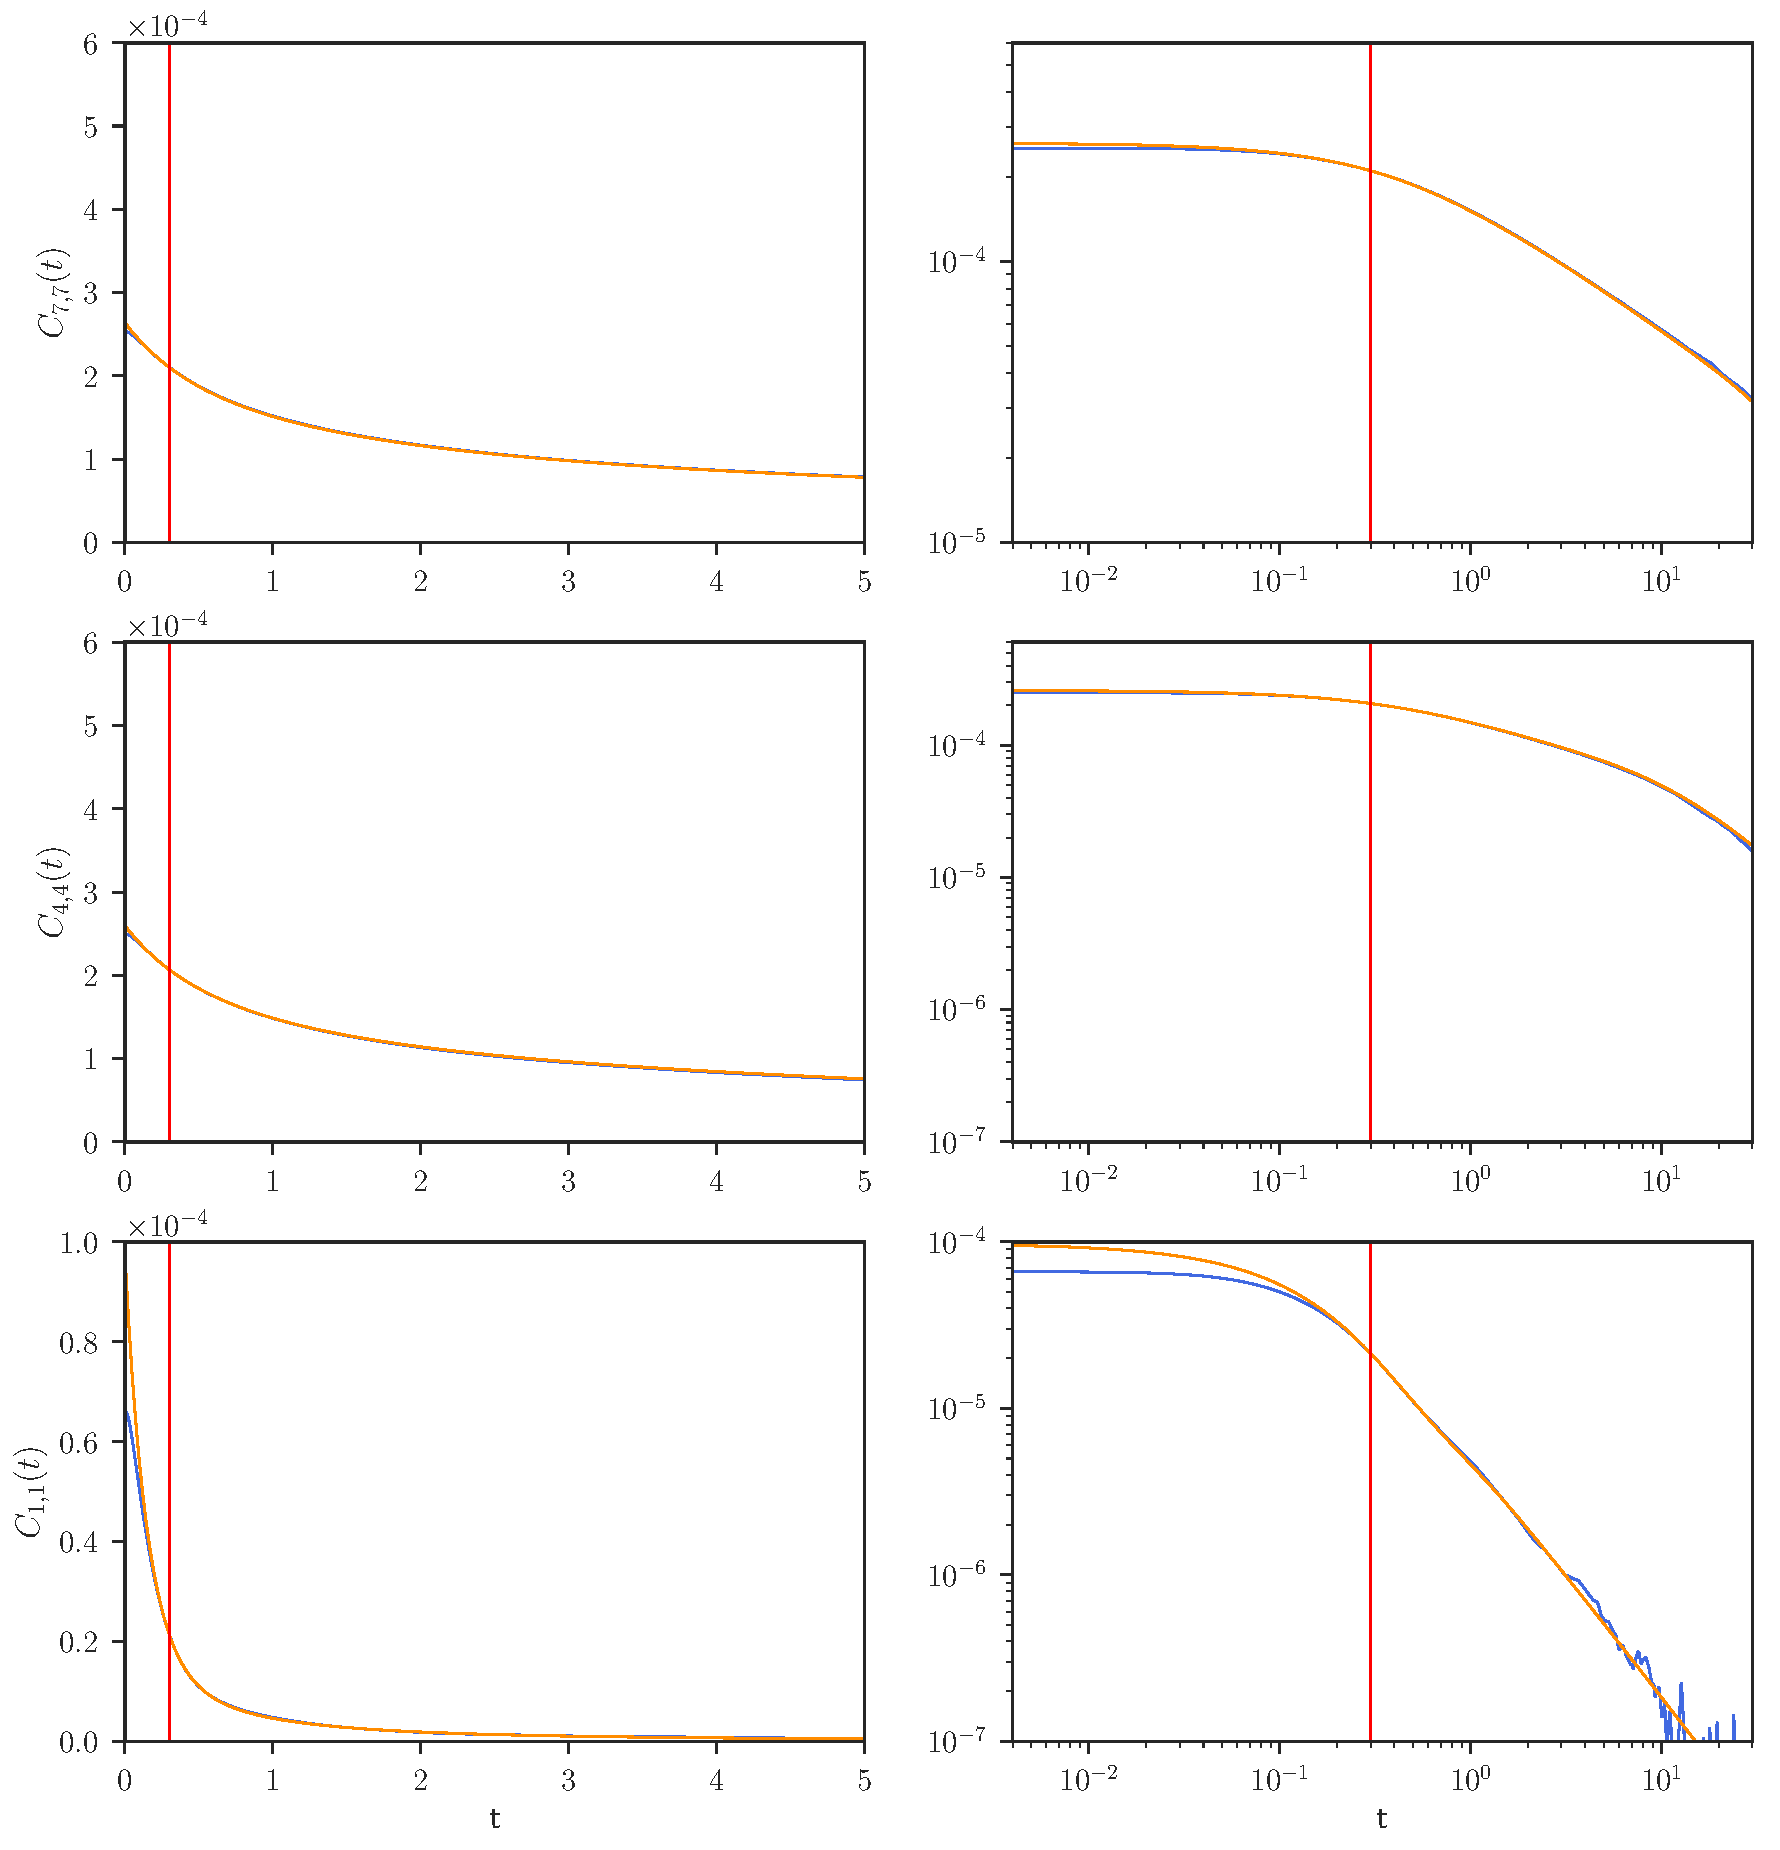
\includegraphics[width=\linewidth]{PredictionsCross-WALLS-17nodes}
\end{figure}
\end{frame}

\begin{frame}{Layering de la densidad}
  El coste de tener una teoría Markoviana válida cerca de las paredes es la pérdida del layering de la densidad. 
\begin{figure}[h!]
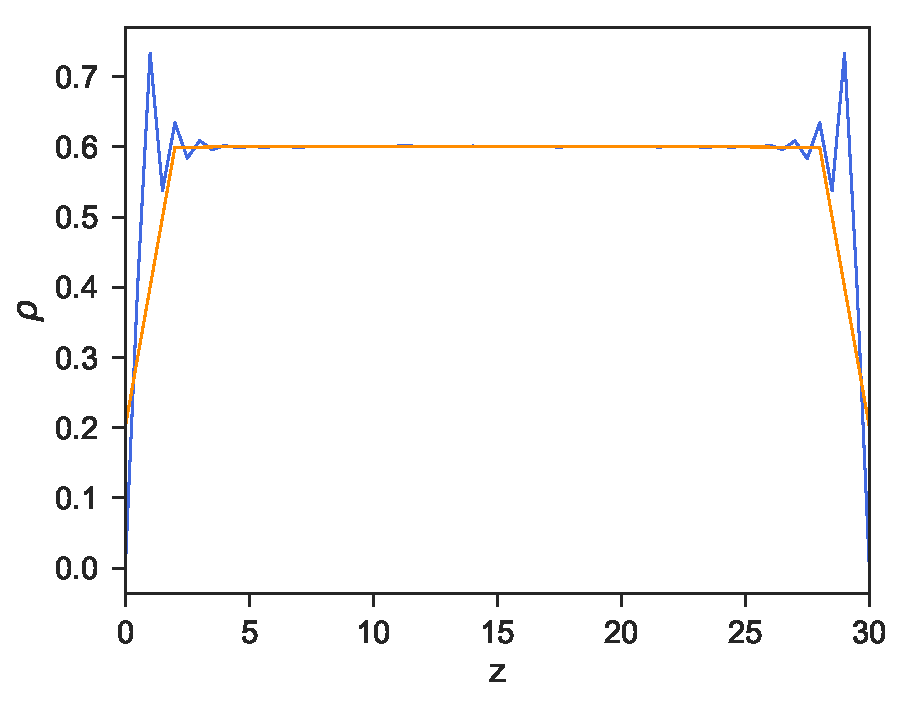
\includegraphics[width=0.6\linewidth]{DensityProfile-WALLS}
\end{figure}
\end{frame}

\metroset{background=dark}
\begin{frame}
  \begin{itemize}
    \item<1-> Autovalores que cortan la recta $y=0$ $\rightarrow$ No puede ser válida la hipótesis Markoviana cerca de la pared.
    \item<2-> Las predicciones en el centro del canal son buenas, pero no cerca de las paredes. 
    \item<3-> Teoría Markoviana válida si el tamaño de bin es superior a la distancia molecular $\rightarrow$ \alert{pérdida del layering}. 
  \item<4-> D. Duque-Zumajo, D. Camargo, J. A. de la Torre, Farid Chejne, and Pep Espa\~nol. Discrete hydrodynamics near solid walls: non-Markovian effects and slip. \textit{Physical Review E}, 2019. 
  \end{itemize}

\end{frame}
\metroset{background=white}





%\begin{frame}{Hoja de ruta}
%  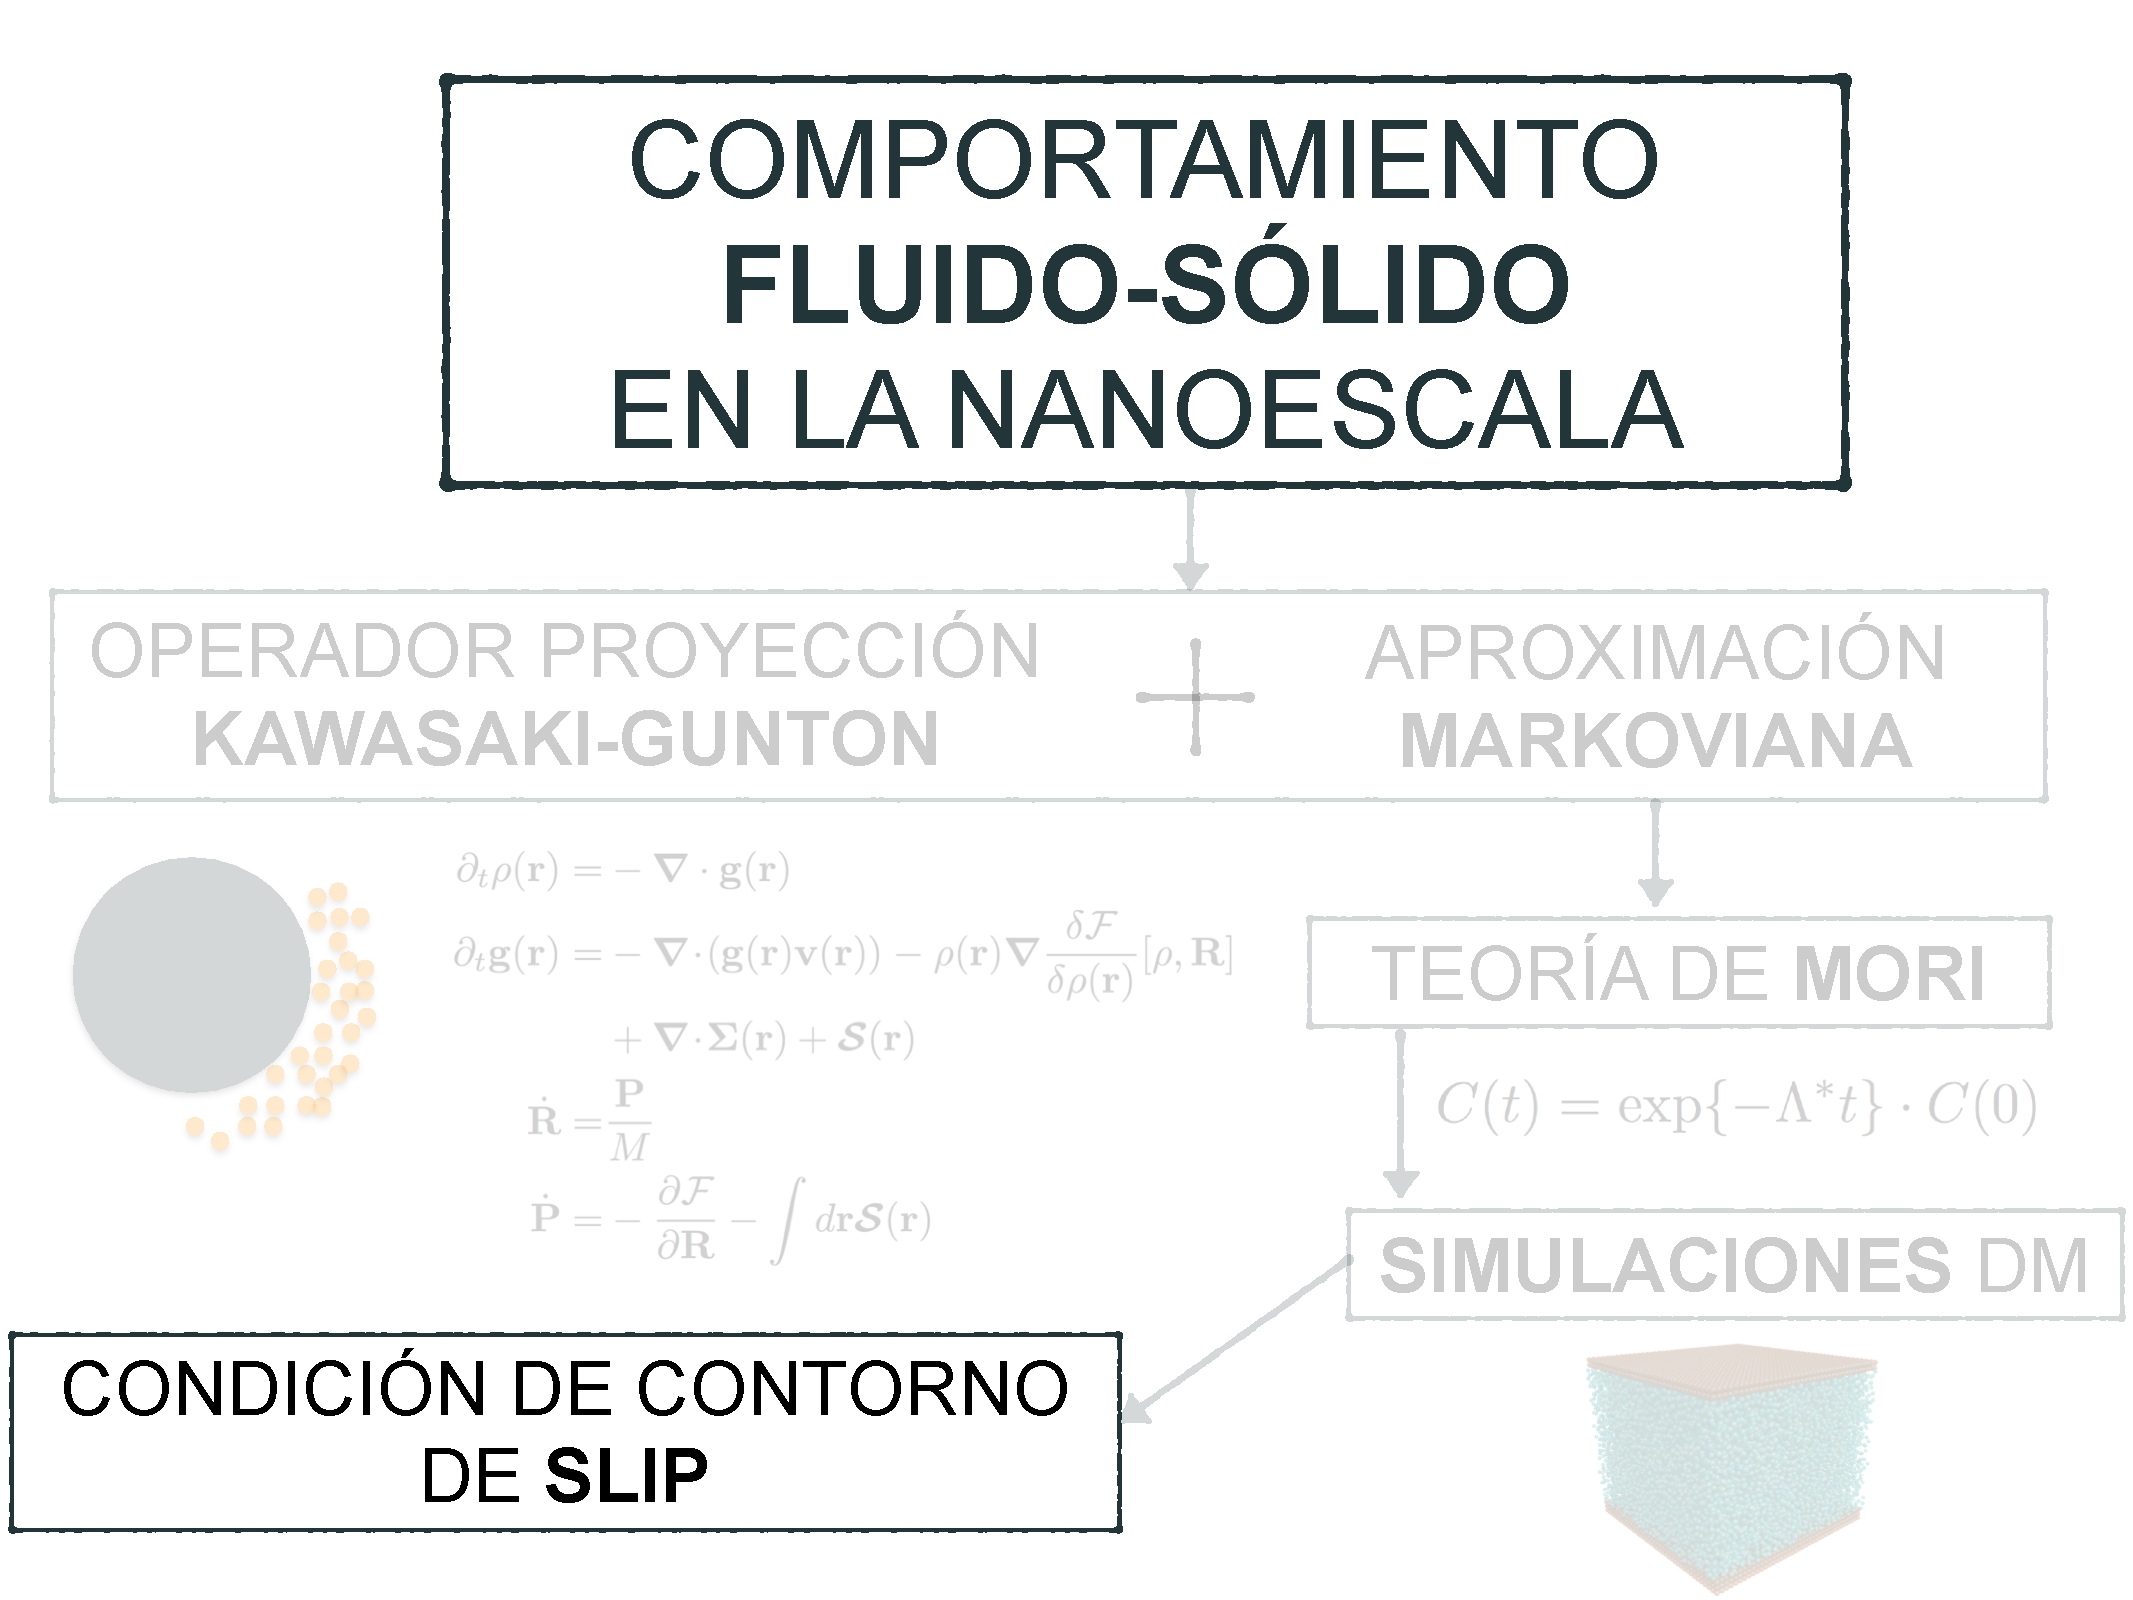
\includegraphics[width=\linewidth]{scheme-thesis-slip}
%\end{frame}


\section{Condición de contorno de slip}

\begin{frame}{Matrices no locales de transporte} 
\begin{align}
\eta_{\mu\nu}(t)
&=\frac{1}{k_BT}\int_0^t dt'
\left\langle \hat{\boldsymbol{\sigma}}^{xz}_{\mu}(t')\hat{\boldsymbol{\sigma}}^{xz}_{\nu}
\right\rangle
\nonumber\\
  G_{\mu\nu}(t)&=\frac{1}{k_BT}\int_0^t dt'
\left\langle\hat{\bf F}^x_\mu(t')
\hat{\boldsymbol{\sigma}}^{xz}_\nu
\right\rangle
\nonumber\\
H_{\mu\nu}(t)&=
\frac{1}{k_BT}\int_0^t dt'
\left\langle\hat{\boldsymbol{\sigma}}^{xz}_\mu(t')\hat{\bf F}^{x}_\nu\right\rangle
\nonumber\\
  \gamma_{\mu\nu}(t)
&=\frac{1}{k_BT}\int_0^t dt'
\left\langle 
\hat{\bf F}^{x}_\mu(t')
\hat{\bf F}^{x}_\nu\right\rangle
\nonumber
\end{align}
\end{frame}









%\begin{frame}{Estrategia}
%  \begin{enumerate}
%    \item<1-> Cálculo de los kernels de viscosidad ($\eta$) y fricción ($G$, $H$, $\gamma$).
%    \item<2-> Fórmula de Green-Kubo corregida sin problema del \textit{plateau}. 
%    \item<3-> Predicción del valor medio del perfil del momento, $g(t)$, con los kernels de transporte corregidos.
%    \item<4-> Condición de contorno de \textit{slip} satisfecha por un \textit{plug flow}.
%    \item<5-> La longitud de \textit{slip} $\gamma$ es independiente del tamaño del canal. 
%    \item<6-> Comparación entre teoría no local y teoría local. 
%  \end{enumerate}
%\end{frame}

\begin{frame}{El problema del plateau}
  \begin{itemize}
    %\item We measure the correlación matrix $C(t)=\llangle \hat{g}(t) \hat{g}^T \rrangle$
%with $\hat{g}^T=(\hat{\bf g}^x_1,\cdots,\hat{\bf g}^x_{\rm bin})$.
    \item<1-> Identidad matemática para la derivada de $C(t)$
\begin{align}
  \frac{d}{dt}C(t)
=-  \int_0^t dt' \llangle i{\cal L}\hat{g}(t') i{\cal L}\hat{g}^T\rrangle
=-  k_BT M(t)
\nonumber
\end{align}
\item<2-> Hemos introducido la integral de Green-Kubo 
\begin{align}
M(t)&= \frac{1}{k_BT}\int_0^t dt'\langle i{\cal L}\hat{g}(t')i{\cal L} \hat{g}^T\rangle
\nonumber
\end{align}
\item<3-> La derivada temporal del momento viene dada por
\begin{align}
  i{\cal L}\hat{g}_\mu &=\hat{F}_\mu-\frac{\hat{\sigma}_\mu-\hat{\sigma}_{\mu-1}}{\Delta z}
\nonumber
\end{align}
%donde
%$\hat{F}_\mu=\hat{\bf                   F}_\mu^x$                  y
%$\hat{\sigma}_\mu=\hat{\boldsymbol{\sigma}}^{xz}_\mu$.
\item<4-> Podemos expresar $M(t)$ en función de los kernels de transporte 
\begin{align}
  {M}(t)&={\cal D}^T\esc{\eta}(t)\esc {\cal D}+{G}(t)\esc {\cal D}+{\cal D}^T\esc{H}(t)+{\gamma}(t)
\nonumber
\end{align}
donde ${\cal D}$ es el operador derivada adelantada. 
%is the bi-diagonal fordward finite difference operator.
  \end{itemize}
\end{frame}

%\begin{frame}{The nonlocal transport matrices} 
%\begin{align}
%\eta_{\mu\nu}(t)
%&=\frac{1}{k_BT}\int_0^t dt'
%\left\langle \hat{\boldsymbol{\sigma}}^{xz}_{\mu}(t')\hat{\boldsymbol{\sigma}}^{xz}_{\nu}
%\right\rangle
%\nonumber\\
%  G_{\mu\nu}(t)&=\frac{1}{k_BT}\int_0^t dt'
%\left\langle\hat{\bf F}^x_\mu(t')
%\hat{\boldsymbol{\sigma}}^{xz}_\nu
%\right\rangle
%\nonumber\\
%H_{\mu\nu}(t)&=
%\frac{1}{k_BT}\int_0^t dt'
%\left\langle\hat{\boldsymbol{\sigma}}^{xz}_\mu(t')\hat{\bf F}^{x}_\nu\right\rangle
%\nonumber\\
%  \gamma_{\mu\nu}(t)
%&=\frac{1}{k_BT}\int_0^t dt'
%\left\langle 
%\hat{\bf F}^{x}_\mu(t')
%\hat{\bf F}^{x}_\nu\right\rangle
%\nonumber
%\end{align}
%\end{frame}

%\begin{frame}{Simulations}
%\begin{figure}[]
%  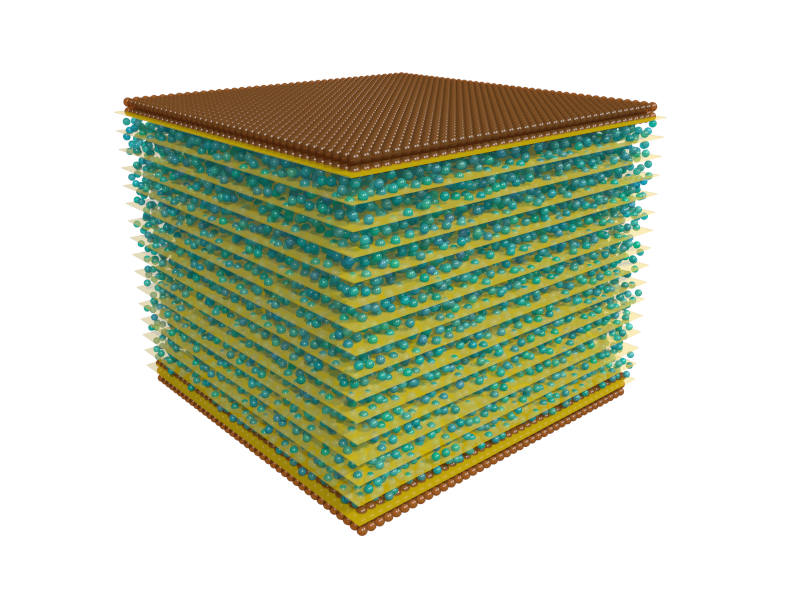
\includegraphics[width=0.5\linewidth]{PRL3_gold2_wo_diffuse}
%\end{figure}
%\begin{figure}[h!]
%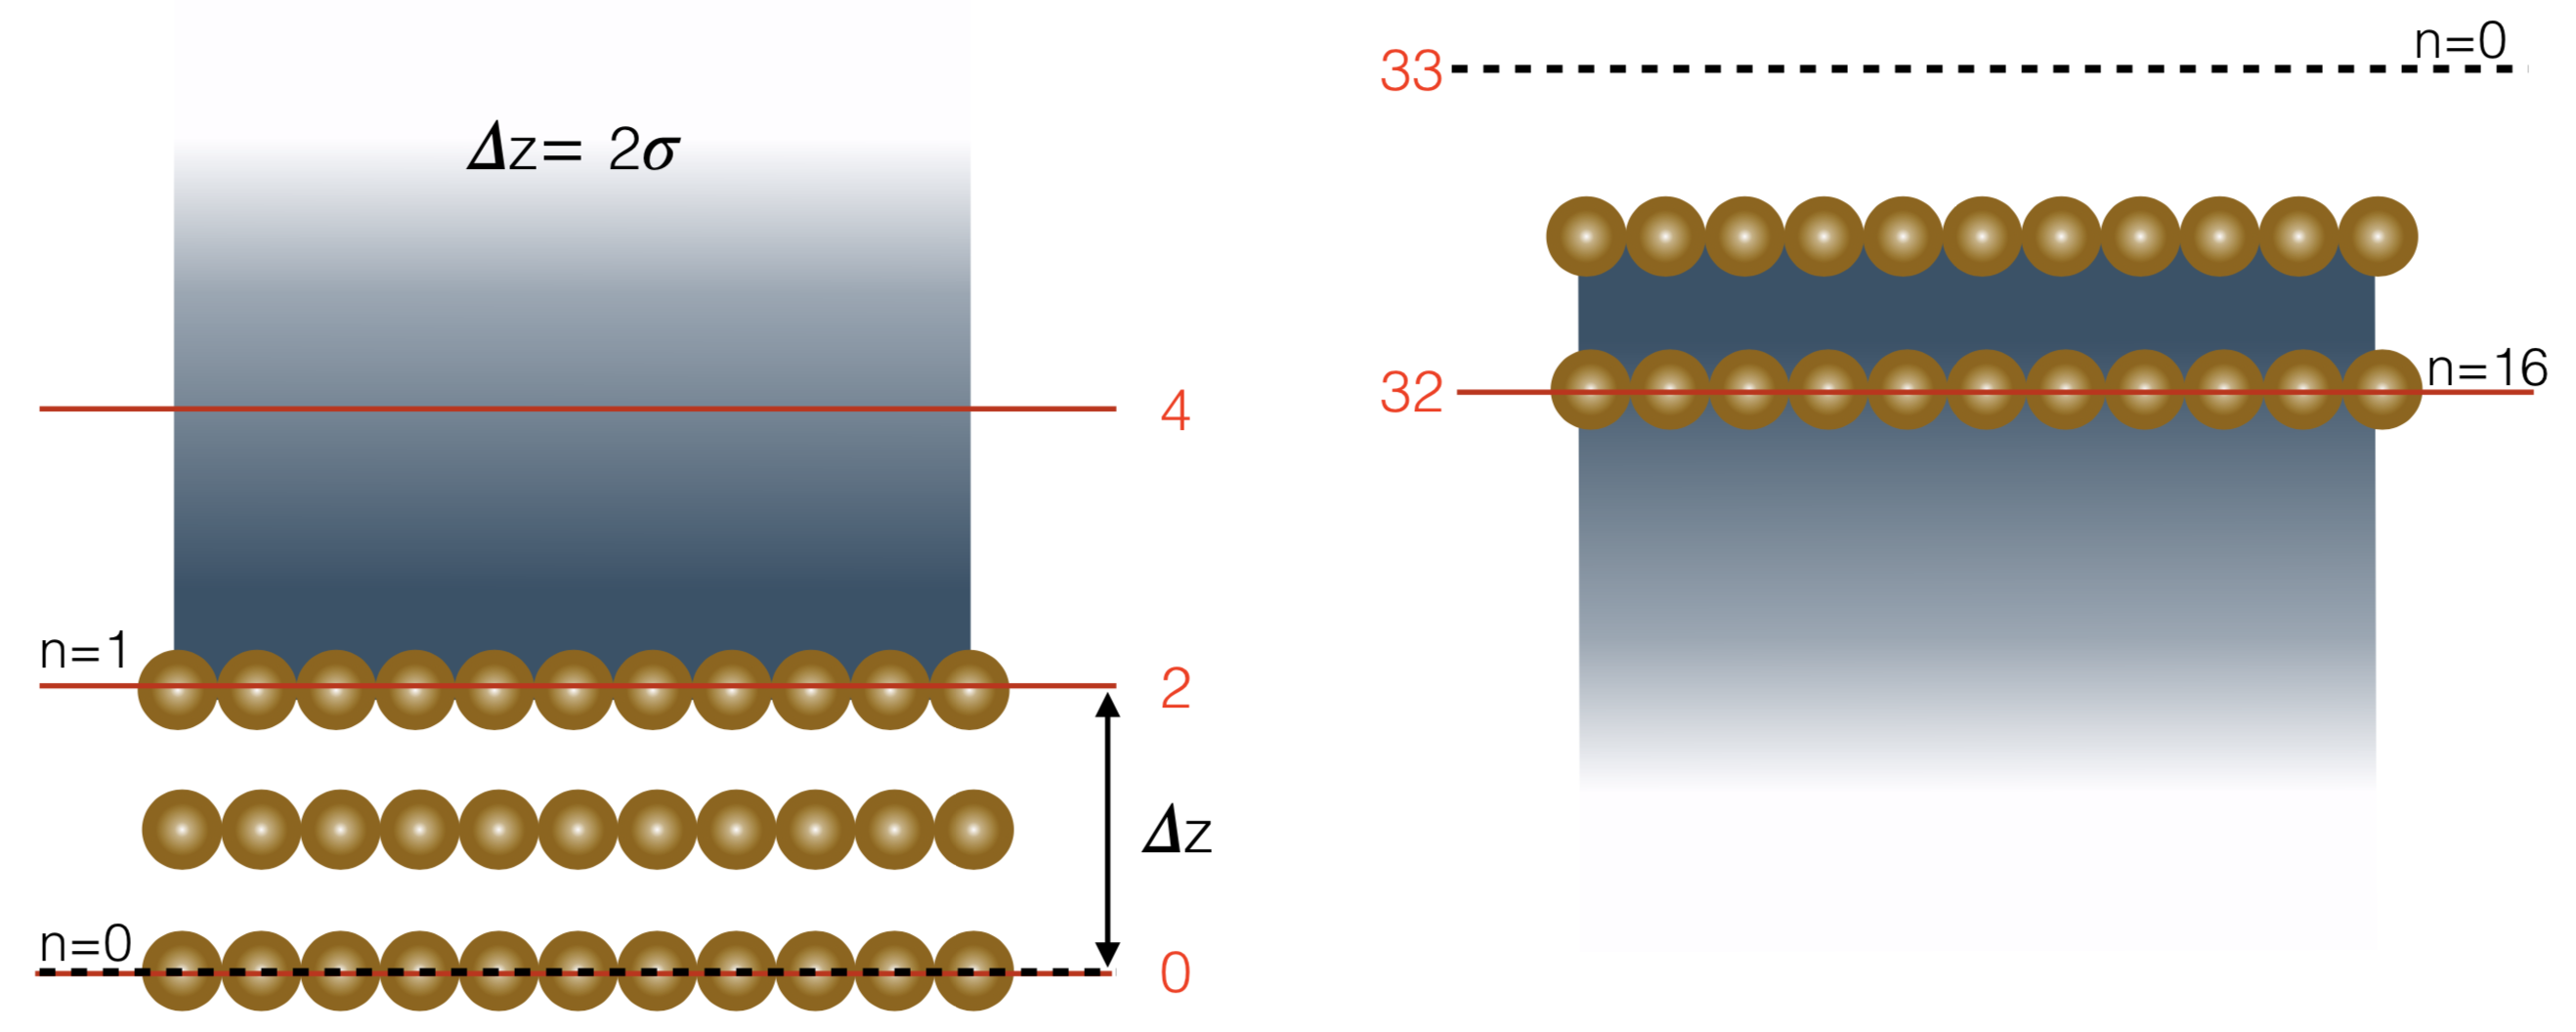
\includegraphics[width=0.8\linewidth]{bin_size-top-bottom_17nodos_cut}
%\end{figure}
%\end{frame}



\begin{frame}{El problema del plateau}
  $\eta_{10,10}(t)$ (centro del canal), $\gamma_{1,1}$ ({\color{blue} azul}) y $\gamma_{2,2}$ ({\color{orange}naranja}). 
\begin{figure}[]
  \includegraphics[scale=0.33]{NoPlateau-WALLS-17nodes}
\end{figure}
\end{frame}

\begin{frame}{Expresión de Green-Kubo corregida}
  \begin{itemize}
    \item<1-> Teoría de Mori con aproximación Markoviana
      \begin{align}
        %\frac{d}{dt}C(t)=-k_BT({\color{red}\cancel{L}} + M^*)\esc C^{-1}(0)\esc C(t)
        \frac{d}{dt}C(t)=-k_BT\esc M^*\esc C^{-1}(0)\esc C(t)
        \nonumber
      \end{align}
    \item<2-> Identidad matemática:  $\frac{d}{dt}C(t)=-k_B T\esc M(t)$
    \item<3-> Fórmula de Green-Kubo corregida  
      %\begin{align}
      $ M^*=M(\tau)\esc {\color{blue}C^{-1}(\tau)\esc C(0)}$
      %\end{align}
      %where $c(\tau)=C^{-1}(0)\esc C(\tau)$
    \item<4-> Evolución de la matriz de correlaciones
      \begin{align}
        \frac{d}{dt}C(t)=-\underbrace{k_BT\esc M(\tau)\esc  C^{-1}(\tau)}_{\Lambda^*}\esc C(t)
        \nonumber
      \end{align}
    \item<5-> Evolución del campo de momento
      \begin{align}
        %\frac{d}{dt}g(t)=-k_BT\esc M(\tau)\esc C^{-1}(\tau)\esc g(t)
        \frac{d}{dt}g(t)=-\Lambda^*\esc g(t)
        \nonumber
      \end{align}
    \item<6-> Evolución de $g(t)$ en función de la velocidad: 
      ${\bf v}^x_\mu=\sum_{\nu}\rho_{\mu\nu}^{-1}{\bf g}^x_\nu$
      \begin{align}
        \frac{d}{dt}g(t)=-{\cal V}\esc M(\tau)\esc \underbrace{{\color{blue}C^{-1}(\tau)\esc C(0)}\esc v(t)}_{\overline{v}(t)}
        %\frac{d}{dt}v(t)=-k_BT\esc M(\tau)\esc C^{-1}(\tau)\esc {\cal V}\esc \underbrace{C^{-1}(\tau)\esc C(0)\esc v(t)}_{\overline{v}(t)}
        \nonumber
      \end{align}
  \end{itemize}
\end{frame}

\begin{frame}{Simulación de un plug flow}
  \begin{itemize}
    \item<1-> Desde una situación de equilibrio añadimos a la velocidad de cada átomo de fluido la misma velocidad $\bf{V}$.
\begin{figure}[]
  \includegraphics[width=0.3\linewidth]{plug_flow}
\end{figure}
\item<2-> Aumenta la energía cinética $\rightarrow$ Aumenta la temperatura.
\item<3-> Reescalamos las velocidades resultantes para mantener el mismo punto termodinámico ($T=2$, $\rho=0.6$).
\item<4-> Medimos $g^x_{\mu}(t)$ en cada uno de los nodos del sistema. 
  %$\boldsymbol{\Delta} {\bf z=2}\boldsymbol{\sigma}$. 16 nodos de fluido. 
%\item<5-> Promediamos 5000 simulaciones inicializadas con diferentes configuraciones. 
  \end{itemize}
\end{frame}

\begin{frame}{Predicciones del plug flow}
  \begin{align}
    g(t)=\exp\{-\Lambda^* (t-\tau)\}\esc g(\tau)
    \nonumber
\end{align}
\begin{figure}[!h]
\includegraphics[width=0.55\linewidth]{gxtPredictions-17nodes-WALLS-defense1}
\end{figure}
  {\color{orange} Predicciones} (con $\tau=0.3$) del {\color{blue} momento medido} para los tiempos $t=1,3,...,21$ (en orden descendente).
\end{frame}

\begin{frame}{Predicciones del plug flow}
      El {\color{blue} momento medido} y las {\color{orange} predicciones} para los nodos $\mu=1, 2,...,8$ en orden ascendente.
\begin{figure}[!h]
\includegraphics[width=\linewidth]{gxtPredictions-17nodes-WALLS-defense2}
\end{figure}
  %\begin{itemize}
    %\item 
    %\item Only after the time in which the transport matrix reached a plateau, y hence a Markovian teoría holds, it is expected that we get correct predictions. 
  %\end{itemize}
\end{frame}


\begin{frame}
  \textbf{Interacción fluido-sólido} a través de \alert{fuerzas de fricción} \\ 
  \begin{center}
  $\downarrow$ \\
  \end{center}
  \textbf{Interacción fluido-sólido} a través de \alert{condiciones de contorno}
\end{frame}

%\begin{frame}{The boundary condition from pillbox argument}
%Boundary slab of made of $B$ bins near one of the walls.
%  \begin{enumerate}
%    \item The momentum obeys the dynamics
%      \begin{align}
%        \frac{d}{dt}g(t)=-k_BT\esc M(\tau)\esc C^{-1}(\tau)\esc g(t)
%        \nonumber
%      \end{align}
%\item The velocity field inside the boundary slab is linear
%\begin{align}
%\overline{\bf v}^x_{\mu}&=  \overline{\bf v}^x_{\rm wall}+\dot{\overline{\gamma}}_{\rm wall}(\mu\Delta z-z_{\rm wall})
%\nonumber
%\end{align}
%      \begin{itemize}
%        \item $z_{\rm wall}$: position of the wall. 
%        \item $\overline{\bf v}^x_{\rm wall}$: velocity at $z_{\rm wall}$.
%        \item $\dot{\overline{\gamma}}_{\rm wall}$: shear rate.
%      \end{itemize}
%\item The force on the boundary slab is vanishingly small. 
%  \end{enumerate}
%The Navier slip boundary condition y the slip length $\delta$
%\begin{align}
%\overline{\bf v}^x_{\rm wall}=\delta\dot{\overline{\gamma}}_{\rm wall}
%  =\frac{\eta-G}{\gamma-H}\dot{\overline{\gamma}}_{\rm wall}
%  \nonumber
%\end{align}
%\end{frame}

\begin{frame}{La condición de contorno}
    %\item Hemos resuelto la ecuación discreta no local para $g^x_{\mu}(t)$ sin hacer referencia a la condición de contorno. 
  \begin{itemize}
    \item \textbf{Derivamos condiciones de contorno cerca de la pared}. 
    \item Para ello seleccionamos una \alert{región de contorno} compuesta por $B$ bines cerca de la pared.
\item[]
  \begin{figure}
    \includegraphics[width=\linewidth]{region_contorno}
  \end{figure}
  \end{itemize}
\end{frame}

\begin{frame}{La condición de contorno}
  \begin{itemize}
    %\item Hemos resuelto la ecuación discreta no local para $g^x_{\mu}(t)$ sin hacer referencia a la condición de contorno. 
    \item<1-> \alert{Región de contorno} compuesta por $B$ bines cerca de la pared.
  \begin{enumerate}
    \item<1-> La evolución del momento obedece la ecuación
      \begin{align}
        \frac{d}{dt}g(t)=-k_BT\esc M(\tau)\esc C^{-1}(\tau)\esc g(t)
        \nonumber
      \end{align}
      %$\rightarrow$ $\tau=0.3$
\item<2-> El campo de velocidad dentro de la región es lineal 
\begin{align}
\overline{\bf v}^x_{\mu}&=  \overline{\bf v}^x_{\rm wall}+\dot{\overline{\gamma}}_{\rm wall}(\mu\Delta z-z_{\rm wall})
\nonumber
\end{align}
      \begin{itemize}
        \item $z_{\rm wall}$: posición de la pared.
        \item $\overline{\bf v}^x_{\rm wall}$: velocidad en  $z_{\rm wall}$.
        \item $\dot{\overline{\gamma}}_{\rm wall}$: gradiente de la velocidad.
          %shear rate
      \end{itemize}
      $\rightarrow$ $B=2$
    \item<3-> La fuerza sobre la región de contorno es muy pequeña. \\
      $\rightarrow$ $t>2$
  \end{enumerate}
%\item<5-> Por \textbf{(2)} escogemos $B=2$ y observamos que \textbf{(3)} se cumple para $t>2$.
\item<4-> Condición de contorno y longitud de slip $\delta$
\begin{align}
\overline{\bf v}^x_{\rm wall}=\delta\dot{\overline{\gamma}}_{\rm wall}
  && \delta=\frac{\eta-G}{\gamma-H}
  \nonumber
\end{align}
  \end{itemize}
\end{frame}

%\begin{frame}{Linear aproximación for the velocity y force on the slab}
%\begin{figure}[!h]
%  \includegraphics[width=0.5\linewidth]{vtCorrected-17nodes-WALLS-defense}
%  \includegraphics[width=0.5\linewidth]{checkMecBalance-17nodes-WALLS-defense}
%\end{figure}
%  \begin{itemize}
%    \item The linear aproximación for the velocity depends on the width of the boundary slab $B$. We choose $B=2$.\\
%\item The force on the slab boundary vanishes for times larger than $t=2$.
%  \end{itemize}
%\end{frame}

\begin{frame}{Validación de la condición de contorno de slip}
  \begin{itemize}
    \item Medimos la longitud de \textit{slip} a través de 
      %$\overline{\bf v}_{\rm wall}(t)$ y $\dot{\overline{\gamma}}_{\rm wall}$
%\begin{align}
 $\delta(t)=\frac{\overline{\bf v}^x_{\rm wall}(t)}{\dot{\overline{\gamma}}_{\rm wall}(t)}$
%\nonumber
%\end{align}
\item La longitud de \textit{slip} 
  %\begin{align}
  $\delta =\frac{\eta -G}{\gamma-H}$
    %\nonumber
  %\end{align}
  \end{itemize}
  \begin{figure}[]
\includegraphics[width=\linewidth]{Slipt-17nodes-WALLS}
  \end{figure}
  \begin{itemize}
    \item La longitud de slip no depende del tamaño del canal (izq.) y es independiente de $\tau$ (dcha.).
  \end{itemize}
\end{frame}

%\begin{frame}{Local hydrodynamic model with boundary conditions}  
%  \begin{itemize}
%    \item The disrete version of the local equation $\partial_t g(z,t)=\nu\frac{\partial^2}{\partial z^2} g(z,t)$
%\begin{align}
%  \frac{d}{dt}g_\mu(t)&=\nu \frac{1}{\Delta z^2}(g_{\mu-1}(t)+g_{\mu+1}(t)-2g_{\mu}(t))
%\nonumber
%\end{align}
%where the kinematic viscosity is $\nu=\frac{\eta}{\rho}$.
%    \item Nonlocal hydrodynamic equation  
%\begin{align}
%  \frac{d}{dt}{\bf g}^x_\mu(t)=&
%-\sum_{\nu} {\cal V}_\nu \frac{\left[\eta_{\mu\nu}-\eta_{\mu-1\nu}-\eta_{\mu\nu-1}+\eta_{\mu-1\nu-1}\right]}{\Delta z^2}\overline{\bf v}^x_\nu \nonumber \\
%  &{\color{red}+\sum_{\nu} {\cal V}_\nu\frac{\left[G_{\mu\nu}-G_{\mu\nu-1}\right]}{\Delta z}\overline{\bf v}^x_\nu
%+\sum_{\nu} {\cal V}_\nu\frac{\left[H_{\mu\nu}-H_{\mu-1\nu}\right]}{\Delta z}
%  \overline{\bf v}^x_\nu}
%\nonumber \\
%  &{\color{red}-\sum_{\nu} {\cal V}_\nu\gamma_{\mu\nu}\overline{\bf v}^x_\nu}
%\nonumber
%\end{align}
%\item We use the slip boundary condition $\overline{\bf v}_{\rm wall}^x=\delta \dot{\overline{\gamma}}_{\rm wall}$ applied at $z_{\rm wall}$.
%  \end{itemize}
%\end{frame}


\begin{frame}{Condición en el contorno con teoría no local}
  \begin{itemize}
    \item[] \alert{Teoría no local} \textbf{sin condiciones de contorno} que nos permite obtener una condición {\bf en} el contorno:  
      \begin{align}
      \overline{\bf v}^x_{\rm wall}(t) = \delta\dot{\overline{\gamma}}_{\rm wall}(t)
        \nonumber
      \end{align}
    %\item[] Hemos observado una condición en el contorno: 
 %$\delta(t)=\frac{\overline{\bf v}^x_{\rm wall}(t)}{\dot{\overline{\gamma}}_{\rm wall}(t)}$
\item[]
  \begin{figure}
    \includegraphics[width=0.45\linewidth]{condiciones_contorno_paredes_recorte}
  \end{figure}
  \end{itemize}
\end{frame}

  \begin{frame}{Condición de contorno en teoría local}
    \begin{itemize}
      \item[] \alert{Teoría local} que tenga en cuenta la presencia del sólido a través de condiciones de contorno:
        \begin{align}
      \overline{\bf v}^x_{\rm wall}(t) = \delta\dot{\overline{\gamma}}_{\rm wall}(t)
        \nonumber
        \end{align}
  \begin{figure}
    \includegraphics[width=0.55\linewidth]{condicion_contorno_recorte}
  \end{figure}
\end{itemize}
\end{frame}


\begin{frame}{Modelo hidrodinámico local con condicion de contorno}  
  \begin{itemize}
    \item<1-> Versión discreta de la ecuación local $\partial_t g(z,t)=\nu\frac{\partial^2}{\partial z^2} g(z,t)$
\begin{align}
  \frac{d}{dt}{\bf g}^x_\mu(t)&=\nu \frac{1}{\Delta z^2}({\bf g}^x_{\mu-1}(t)+{\bf g}^x_{\mu+1}(t)-2{\bf g}^x_{\mu}(t))
\nonumber
\end{align}
donde la viscosidad cinemática es $\nu=\frac{\eta}{\rho}$.
    \item<2-> Ecuación hidrodinámica no local 
\begin{align}
  \frac{d}{dt}{\bf g}^x_\mu(t)=&
-\sum_{\nu} {\cal V}_\nu \frac{\left[\eta_{\mu\nu}-\eta_{\mu-1\nu}-\eta_{\mu\nu-1}+\eta_{\mu-1\nu-1}\right]}{\Delta z^2}\overline{\bf v}^x_\nu \nonumber \\
  &{\color{red}+\sum_{\nu} {\cal V}_\nu\frac{\left[G_{\mu\nu}-G_{\mu\nu-1}\right]}{\Delta z}\overline{\bf v}^x_\nu
+\sum_{\nu} {\cal V}_\nu\frac{\left[H_{\mu\nu}-H_{\mu-1\nu}\right]}{\Delta z}
  \overline{\bf v}^x_\nu}
\nonumber \\
  &{\color{red}-\sum_{\nu} {\cal V}_\nu\gamma_{\mu\nu}\overline{\bf v}^x_\nu}
\nonumber
\end{align}
\item<3-> Empleamos la condición de contorno de \textit{slip} $\overline{\bf v}_{\rm wall}^x=\delta \dot{\overline{\gamma}}_{\rm wall}$ aplicada en $z_{\rm wall}$.
  \end{itemize}
\end{frame}



\begin{frame}{Predicciones locales}
%\begin{align}
% g(t)&=\exp\{\nu \Delta' (t-\tau)\}g(\tau)
%\nonumber
%\end{align}
%with $\Delta'$ the Laplacian operator for slip boundary condition.
\begin{figure}[]
\includegraphics[width=\linewidth]{gxtLocalPrediction-17nodes-WALLS-defense}
\end{figure}
  {\color{orange} Predicción local}
  y {\color{blue} medición} del perfil del momento.\\
  Izq.: $t=0.3,0.6,\cdots2.1$ en orden descendente.\\
  Dcha.: $t=5,7,\cdots,29$  en orden descendente.
\end{frame}

\begin{frame}{Comparación de errores entre teorías local y no local}
  \begin{align}
  err_\mu(t)=  g_\mu(t)-g^{\rm predict}_\mu(t)
    \nonumber
  \end{align}
    \begin{figure}
\includegraphics[width=\linewidth]{errors-17nodes-WALLS-defense}
\end{figure}
  %\begin{itemize}
    %\item The local teoría gives higher errors. 
    %\item The slip boundary condition used to predict the flow does not hold. 
    %\item It is necessary to consider the explicit interaction between the solid y the fluid through the surface irreversible forces containing the transport kernels $G_{\mu\nu}$,$H_{\mu\nu}$,$\gamma_{\mu\nu}$.
    %\item While the local prediction with the slip boundary condition is acceptable, nonlocal effects are appreciable. 
  %\end{itemize}
\end{frame}

\metroset{background=dark}
\begin{frame}
  \begin{itemize}
    \item<1-> Fórmula de Green-Kubo corregida que evita el \alert{problema del plateau} en los kernels de transporte. 
    %\item<2-> Buenas predicciones del momento de un \textit{\alert{plug flow}} con corrección de Green-Kubo. 
    \item<2-> \alert{Condición de contorno} a partir de la teoría no local. 
    \item<3-> Errores en la teoría local debido a \alert{efectos no locales} que no captura.  
    \item<4-> La \alert{longitud de slip} no depende de la geometría del sistema. 
    \item<5-> Pep Espa\~nol, J.A.de la Torre, and D.Duque-Zumajo. Solution to the plateau problem in the Green-Kubo formula. \textit{Physical Review E}, 99(2), 2019.
    \item<5-> D. Duque-Zumajo, J.A. de la Torre, D. Camargo, and Pep Español. Slip in nanohydrodynamics. \textit{Physical Review Letters}, 2019. 
  \end{itemize}

\end{frame}
\metroset{background=white}


\begin{frame}{Conclusiones}
  \begin{enumerate}
    \item<1-> DDFT para un fluido en contacto con una esfera sólida. 
    \item<2-> Ecuaciones de la hidrodinámica para un fluido en contacto con paredes planas. 
    \item<3-> Si la hipótesis Markoviana es válida las correlaciones decaen de forma exponencial. 
    \item<4-> Efectos no Markovianos cerca de la pared cuando el tamaño de bin es inferior a la distancia molecular. 
    \item<5-> Fórmula de Green-Kubo corregida para evitar el problema del \textit{plateau}.
    \item<6-> Excelentes predicciones del momento de un \textit{plug flow} empleando los kernels de transporte corregidos. 
    \item<7-> La longitud de slip no depende de la geometría del sistema.  
  \end{enumerate}
\end{frame}


%\begin{frame}{Publicaciones relacionadas}
%  \begin{itemize}
%      \begin{small}
%    \item D.Camargo, J.A. de la Torre, {\bf D.Duque-Zumajo}, P.Espa\~nol, R.Delgado-Buscalioni, and F. Chejne. Nanoscale hydrodynamics near solids. \textit{Journal of Chemical Physics}, 148(6), 2018.
%    \item P.Espa\~nol, J.A.de la Torre, and {\bf D.Duque-Zumajo}. Solution to the plateau problem in the Green-Kubo formula. \textit{Physical Review E}, 99(2), 2019.
%    \item {\bf D. Duque-Zumajo}, D. Camargo, J. A. de la Torre, F. Chejne, and Pep Espa\~nol. Discrete hydrodynamics for planar flows with confining walls. \textit{Physical Review E}, 2019.
%  \item {\bf D. Duque-Zumajo}, J. A. de la Torre, and Pep Espa\~nol. Slip and non-Markovian effects in nanohydrodynamics (in preparation). \textit{Physical Review Letters}, 2019. 
%  \item {\bf D. Duque-Zumajo}, D. Camargo, J. A. de la Torre, Farid Chejne, and Pep Espa\~nol. Discrete hydrodynamics near solid walls: non-Markovian effects and slip (in preparation). \textit{Physical Review E}, 2019. 
%      \end{small}
%  \end{itemize}
%\end{frame}

\begin{frame}{Trabajo futuro}
  \begin{enumerate}
        \item Estudio de los efectos no Markovianos.
      \begin{itemize}
        \item Modelos más realistas para el sólido. 
        \item Modificar el punto termodinámico.  
        %\item Analizar si la hidrofobicidad y la hidrofilicidad afectan a las conclusiones.
      \end{itemize}
    \item Teoría no isoterma. 
      \begin{itemize}
        %\item Nuevas variables relevantes
%\begin{align}
%  \hat{e}_{\bf r}(z) = \sum_i^N e_i\delta({\bf r}-{\bf q}_i) &&  \hat{E}(z)=\sum_{i'}^{N'}e_{i'}
%  \nonumber
%\end{align}
%\item Resolver el problema de as condiciones de contorno térmicas. 
    \item Transporte de calor entre sólidos y fluidos.
    \item Nanopartículas y sales fundidas $\rightarrow$ Aplicación en almacenamiento térmico en la industria termosolar.
      \end{itemize}
  \end{enumerate}
\end{frame}

\begin{frame}
\begin{figure}
\includegraphics[width=0.2\linewidth]{logo}
\end{figure}
  \vspace{0.5cm}  
\begin{center}
\textit{Nanoscale hydrodynamics near solids}\\
Julio 2019\\
Diego Duque Zumajo
\end{center}

\end{frame}

\begin{frame}{Dual basis functions y mass matrix}
  \begin{itemize}
  \item We can contruct continuum y discrete fields from dual basis functions $\delta_{\mu}({\bf r})$ y $\psi_\mu({\bf r})$ 
    \begin{align}
      v_\mu=\int d{\bf r}v({\bf r})\delta_\mu({\bf r}),&&
        \overline{v}({\bf r}) =\sum_{\mu}v_\mu\psi_\mu({\bf r})
    \nonumber
    \end{align}
    \item The usual mass matrix of the finite element method is
      \begin{align}
      M^\Phi_{\mu\nu}&=\llg\Phi_\mu\Phi_\nu\rlg  
      \nonumber
      \end{align}
      where we have introduce the notation $\llg\cdots\rlg=\int d{\bf r}...$
    \item We introduce the discrete velocity field in terms of $M^\Phi_{\mu\nu}$
      \begin{align}
        \tilde{{\bf v}}_{\mu}=\sum_{\nu}{\cal V}_{\mu}[M^{\Phi}]^{-1}_{\mu\nu}{\bf v}_{\nu}
        \nonumber
      \end{align}
  \end{itemize}
\end{frame}

\begin{frame}{Validez hipótesis Markoviana}
  \begin{itemize}
    \item Ecuación de Mori
\begin{align}
  \frac{d}{dt}C(t)&=-L\esc C^{-1}(0)\esc C(t)
  -\int_0^tdt' \Gamma(t-t')\esc C^{-1}(0)\esc  C(t')
\end{align}
\item Mori con aproximación Markoviana
  \begin{align}
    \frac{d}{dt}C(t)=-\Lambda^*\esc C(t)=-(L+M^*)\esc C^{-1}(0)\esc C(t)
  \end{align}

\item Para $t=0$ (1) quedaría
  \begin{align}
  \frac{d}{dt}C(0)&=-L
    \nonumber
\end{align}

\item Esto implica por (2) 
  \begin{align}
  M^*=0
  \end{align}
\end{itemize}
\end{frame}

\begin{frame}{Matriz $\tilde{\Lambda}$}
  \begin{itemize}
    \item {\color{blue} Base de $C(t)$ en $t=0.15$.}
    \item {\color{green} Base de $C(t)$ en $t=0.30$.}
    \item {\color{orange} Base de $C(t)$ evolucionando con el tiempo.}
  \end{itemize}
  \begin{figure}
    \includegraphics[width=0.7\linewidth]{LambdatBasis-WALLS-66nodes}
  \end{figure}
\end{frame}

\begin{frame}{Perfil de velocidad}
  $t=1,3,...23$.
\begin{align}
  \overline{\bf v}^x_\mu=\sum_{\nu}\overline{\rho}_{\mu\nu}^{-1}{\bf g}^x_\nu, &&
  \overline{\rho}_{\mu\nu}=\frac{C_{\mu\nu}(\tau)}{k_BT}  {\cal V}_\mu
  \nonumber
\end{align}

  \begin{center}
  \includegraphics[width=0.7\linewidth]{vtCorrected-17nodes-WALLS-defense}
  \end{center}
\end{frame}


\begin{frame}{Definición de $\eta$, $G$, $\gamma$, $H$}
\begin{align}
  \eta&= \sum^{N_{\rm bin}}_{\nu=1} {\cal V}_\nu \eta_{B\nu}
\nonumber\\
G &=  \frac{1}{S} \sum^{N_{\rm bin}}_{\nu=1} {\cal V}_\nu \sum^{B}_{\mu=1}{\cal V}_\mu G_{\mu\nu}
\nonumber\\
\gamma&=  \frac{1}{S}\sum^{N_{\rm bin}}_{\nu=1}{\cal V}_\nu\sum^{B}_{\mu=1}{\cal V}_\mu \gamma_{\mu\nu}
\nonumber\\
H&= \sum^{N_{\rm bin}}_{\nu=1} {\cal V}_\nu H_{B\nu}
\nonumber
\end{align}
\end{frame}

\begin{frame}{Definición de $\eta$, $G$, $\gamma$, $H$}
\begin{align}
\eta&= \frac{1}{k_BT}\int_0^{\tau} dt
\left\langle  \hat{\boldsymbol{\sigma}}^{xz}_{B}(t) \hat{\boldsymbol{\sigma}}^{xz}\right\rangle^{\rm eq}
\nonumber\\
G &=   \frac{1}{Sk_BT}\int_0^{\tau} dt
\left\langle  \hat{\bf F}^{x}(t) \hat{\boldsymbol{\sigma}}^{xz}\right\rangle^{\rm eq}
\nonumber\\
H &=   \frac{1}{k_BT}\int_0^{\tau} dt
\left\langle  \hat{\boldsymbol{\sigma}}^{xz}_{B}(t) \hat{\bf F}^{x}\right\rangle^{\rm eq}
\nonumber\\
\gamma&= 
\frac{1}{Sk_BT}\int_0^{\tau} dt
\left\langle  \hat{\bf F}^{x}(t)\hat{\bf F}^{x}\right\rangle^{\rm eq}
\nonumber
\end{align}


\end{frame}

\begin{frame}{Matrices de transporte para distintos valores de B}
\includegraphics[width=\linewidth]{transportMatrices-17nodes-WALLS}
\end{frame}

\begin{frame}{¿Cómo depende $\eta'$ y $\gamma`$ de $\tau$?}
  \begin{align}
    \delta=\frac{\eta'}{\gamma'}
    \nonumber
  \end{align}
  \begin{align}
    \eta'=\eta-G && \gamma'=\gamma-H
   \nonumber 
  \end{align}
  \begin{center}
\includegraphics[scale=0.41]{tauDependenceSlip-17nodes-WALLS}
  \end{center}
\end{frame}

\end{document}
